%%%%%%%%%%%%%%%%%%%%%%%%%%%%%%%%%%%%%%%
% The Legrand Orange Book
% LaTeX Template
% Version 2.4 (26/09/2018)
%
% This template was downloaded from:
% http://www.LaTeXTemplates.com
%
% Original author:
% Mathias Legrand (legrand.mathias@gmail.com) with modifications by:
% Vel (vel@latextemplates.com)
%
% License:
% CC BY-NC-SA 3.0 (http://creativecommons.org/licenses/by-nc-sa/3.0/)
%
% Compiling this template:
% This template uses biber for its bibliography and makeindex for its index.
% When you first open the template, compile it from the command line with the 
% commands below to make sure your LaTeX distribution is configured correctly:
%
% 1) pdflatex main
% 2) makeindex main.idx -s StyleInd.ist
% 3) biber main
% 4) pdflatex main x 2
%
% After this, when you wish to update the bibliography/index use the appropriate
% command above and make sure to compile with pdflatex several times 
% afterwards to propagate your changes to the document.
%
% This template also uses a number of packages which may need to be
% updated to the newest versions for the template to compile. It is strongly
% recommended you update your LaTeX distribution if you have any
% compilation errors.
%
% Important note:
% Chapter heading images should have a 2:1 width:height ratio,
% e.g. 920px width and 460px height.
%
%%%%%%%%%%%%%%%%%%%%%%%%%%%%%%%%%%%%%%%%%

%----------------------------------------------------------------------------------------
%	PACKAGES AND OTHER DOCUMENT CONFIGURATIONS
%----------------------------------------------------------------------------------------

\documentclass[11pt,fleqn]{book} % Default font size and left-justified equations

%%%%%%%%%%%%%%%%%%%%%%%%%%%%%%%%%%%%%%%%%
% The Legrand Orange Book
% Structural Definitions File
% Version 2.1 (26/09/2018)
%
% Original author:
% Mathias Legrand (legrand.mathias@gmail.com) with modifications by:
% Vel (vel@latextemplates.com)
% 
% This file was downloaded from:
% http://www.LaTeXTemplates.com
%
% License:
% CC BY-NC-SA 3.0 (http://creativecommons.org/licenses/by-nc-sa/3.0/)
%
%%%%%%%%%%%%%%%%%%%%%%%%%%%%%%%%%%%%%%%%%

%----------------------------------------------------------------------------------------
%	VARIOUS REQUIRED PACKAGES AND CONFIGURATIONS
%----------------------------------------------------------------------------------------

\usepackage{graphicx} % Required for including pictures
\graphicspath{{Pictures/}} % Specifies the directory where pictures are stored

\usepackage{lipsum} % Inserts dummy text

\usepackage{tikz} % Required for drawing custom shapes

\usepackage[english]{babel} % English language/hyphenation

\usepackage{enumitem} % Customize lists
\setlist{nolistsep} % Reduce spacing between bullet points and numbered lists

\usepackage{booktabs} % Required for nicer horizontal rules in tables

\usepackage{xcolor} % Required for specifying colors by name
\definecolor{ocre}{RGB}{243,102,25} % Define the orange color used for highlighting throughout the book

%----------------------------------------------------------------------------------------
%	MARGINS
%----------------------------------------------------------------------------------------

\usepackage{geometry} % Required for adjusting page dimensions and margins

\geometry{
	paper=a4paper, % Paper size, change to letterpaper for US letter size
	top=3cm, % Top margin
	bottom=3cm, % Bottom margin
	left=3cm, % Left margin
	right=3cm, % Right margin
	headheight=14pt, % Header height
	footskip=1.4cm, % Space from the bottom margin to the baseline of the footer
	headsep=10pt, % Space from the top margin to the baseline of the header
	%showframe, % Uncomment to show how the type block is set on the page
}

%----------------------------------------------------------------------------------------
%	FONTS
%----------------------------------------------------------------------------------------

\usepackage{avant} % Use the Avantgarde font for headings
%\usepackage{times} % Use the Times font for headings
\usepackage{mathptmx} % Use the Adobe Times Roman as the default text font together with math symbols from the Sym­bol, Chancery and Com­puter Modern fonts

\usepackage{microtype} % Slightly tweak font spacing for aesthetics
\usepackage[utf8]{inputenc} % Required for including letters with accents
\usepackage[T1]{fontenc} % Use 8-bit encoding that has 256 glyphs

%----------------------------------------------------------------------------------------
%	BIBLIOGRAPHY AND INDEX
%----------------------------------------------------------------------------------------

\usepackage[style=numeric,citestyle=numeric,sorting=nyt,sortcites=true,autopunct=true,babel=hyphen,hyperref=true,abbreviate=false,backref=true,backend=biber]{biblatex}
\addbibresource{bibliography.bib} % BibTeX bibliography file
\defbibheading{bibempty}{}

\usepackage{calc} % For simpler calculation - used for spacing the index letter headings correctly
\usepackage{makeidx} % Required to make an index
\makeindex % Tells LaTeX to create the files required for indexing

%----------------------------------------------------------------------------------------
%	MAIN TABLE OF CONTENTS
%----------------------------------------------------------------------------------------

\usepackage{titletoc} % Required for manipulating the table of contents

\contentsmargin{0cm} % Removes the default margin

% Part text styling (this is mostly taken care of in the PART HEADINGS section of this file)
\titlecontents{part}
	[0cm] % Left indentation
	{\addvspace{20pt}\bfseries} % Spacing and font options for parts
	{}
	{}
	{}

% Chapter text styling
\titlecontents{chapter}
	[1.25cm] % Left indentation
	{\addvspace{12pt}\large\sffamily\bfseries} % Spacing and font options for chapters
	{\color{ocre!60}\contentslabel[\Large\thecontentslabel]{1.25cm}\color{ocre}} % Formatting of numbered sections of this type
	{\color{ocre}} % Formatting of numberless sections of this type
	{\color{ocre!60}\normalsize\;\titlerule*[.5pc]{.}\;\thecontentspage} % Formatting of the filler to the right of the heading and the page number

% Section text styling
\titlecontents{section}
	[1.25cm] % Left indentation
	{\addvspace{3pt}\sffamily\bfseries} % Spacing and font options for sections
	{\contentslabel[\thecontentslabel]{1.25cm}} % Formatting of numbered sections of this type
	{} % Formatting of numberless sections of this type
	{\hfill\color{black}\thecontentspage} % Formatting of the filler to the right of the heading and the page number

% Subsection text styling
\titlecontents{subsection}
	[1.25cm] % Left indentation
	{\addvspace{1pt}\sffamily\small} % Spacing and font options for subsections
	{\contentslabel[\thecontentslabel]{1.25cm}} % Formatting of numbered sections of this type
	{} % Formatting of numberless sections of this type
	{\ \titlerule*[.5pc]{.}\;\thecontentspage} % Formatting of the filler to the right of the heading and the page number

% Figure text styling
\titlecontents{figure}
	[1.25cm] % Left indentation
	{\addvspace{1pt}\sffamily\small} % Spacing and font options for figures
	{\thecontentslabel\hspace*{1em}} % Formatting of numbered sections of this type
	{} % Formatting of numberless sections of this type
	{\ \titlerule*[.5pc]{.}\;\thecontentspage} % Formatting of the filler to the right of the heading and the page number

% Table text styling
\titlecontents{table}
	[1.25cm] % Left indentation
	{\addvspace{1pt}\sffamily\small} % Spacing and font options for tables
	{\thecontentslabel\hspace*{1em}} % Formatting of numbered sections of this type
	{} % Formatting of numberless sections of this type
	{\ \titlerule*[.5pc]{.}\;\thecontentspage} % Formatting of the filler to the right of the heading and the page number

%----------------------------------------------------------------------------------------
%	MINI TABLE OF CONTENTS IN PART HEADS
%----------------------------------------------------------------------------------------

% Chapter text styling
\titlecontents{lchapter}
	[0em] % Left indentation
	{\addvspace{15pt}\large\sffamily\bfseries} % Spacing and font options for chapters
	{\color{ocre}\contentslabel[\Large\thecontentslabel]{1.25cm}\color{ocre}} % Chapter number
	{}  
	{\color{ocre}\normalsize\sffamily\bfseries\;\titlerule*[.5pc]{.}\;\thecontentspage} % Page number

% Section text styling
\titlecontents{lsection}
	[0em] % Left indentation
	{\sffamily\small} % Spacing and font options for sections
	{\contentslabel[\thecontentslabel]{1.25cm}} % Section number
	{}
	{}

% Subsection text styling (note these aren't shown by default, display them by searchings this file for tocdepth and reading the commented text)
\titlecontents{lsubsection}
	[.5em] % Left indentation
	{\sffamily\footnotesize} % Spacing and font options for subsections
	{\contentslabel[\thecontentslabel]{1.25cm}}
	{}
	{}

%----------------------------------------------------------------------------------------
%	HEADERS AND FOOTERS
%----------------------------------------------------------------------------------------

\usepackage{fancyhdr} % Required for header and footer configuration

\pagestyle{fancy} % Enable the custom headers and footers

\renewcommand{\chaptermark}[1]{\markboth{\sffamily\normalsize\bfseries\chaptername\ \thechapter.\ #1}{}} % Styling for the current chapter in the header
\renewcommand{\sectionmark}[1]{\markright{\sffamily\normalsize\thesection\hspace{5pt}#1}{}} % Styling for the current section in the header

\fancyhf{} % Clear default headers and footers
\fancyhead[LE,RO]{\sffamily\normalsize\thepage} % Styling for the page number in the header
\fancyhead[LO]{\rightmark} % Print the nearest section name on the left side of odd pages
\fancyhead[RE]{\leftmark} % Print the current chapter name on the right side of even pages
%\fancyfoot[C]{\thepage} % Uncomment to include a footer

\renewcommand{\headrulewidth}{0.5pt} % Thickness of the rule under the header

\fancypagestyle{plain}{% Style for when a plain pagestyle is specified
	\fancyhead{}\renewcommand{\headrulewidth}{0pt}%
}

% Removes the header from odd empty pages at the end of chapters
\makeatletter
\renewcommand{\cleardoublepage}{
\clearpage\ifodd\c@page\else
\hbox{}
\vspace*{\fill}
\thispagestyle{empty}
\newpage
\fi}

%----------------------------------------------------------------------------------------
%	THEOREM STYLES
%----------------------------------------------------------------------------------------

\usepackage{amsmath,amsfonts,amssymb,amsthm} % For math equations, theorems, symbols, etc

\newcommand{\intoo}[2]{\mathopen{]}#1\,;#2\mathclose{[}}
\newcommand{\ud}{\mathop{\mathrm{{}d}}\mathopen{}}
\newcommand{\intff}[2]{\mathopen{[}#1\,;#2\mathclose{]}}
\renewcommand{\qedsymbol}{$\blacksquare$}
\newtheorem{notation}{Notation}[chapter]

% Boxed/framed environments
\newtheoremstyle{ocrenumbox}% Theorem style name
{0pt}% Space above
{0pt}% Space below
{\normalfont}% Body font
{}% Indent amount
{\small\bf\sffamily\color{ocre}}% Theorem head font
{}% Punctuation after theorem head
{0.0em}% Space after theorem head
{\small\sffamily\color{ocre}% Theorem text (e.g. Theorem 2.1)
\thmnote{\nobreakspace\the\thm@notefont\sffamily\bfseries\color{black}---\nobreakspace#3.}} % Optional theorem note

\newtheoremstyle{blacknumex}% Theorem style name
{5pt}% Space above
{5pt}% Space below
{\normalfont}% Body font
{} % Indent amount
{\small\bf\sffamily}% Theorem head font
{}% Punctuation after theorem head
{0.00em}% Space after theorem head
{\small\sffamily{\tiny\ensuremath{\blacksquare}}% Theorem text (e.g. Theorem 2.1)
\thmnote{\nobreakspace\the\thm@notefont\sffamily\bfseries---\nobreakspace#3.}}% Optional theorem note

\newtheoremstyle{blacknumbox} % Theorem style name
{0pt}% Space above
{0pt}% Space below
{\normalfont}% Body font
{}% Indent amount
{\small\bf\sffamily}% Theorem head font
{}% Punctuation after theorem head
{0.00em}% Space after theorem head
{\small\sffamily% Theorem text (e.g. Theorem 2.1)
\thmnote{\nobreakspace\the\thm@notefont\sffamily\bfseries---\nobreakspace#3.}}% Optional theorem note

% Non-boxed/non-framed environments
\newtheoremstyle{ocrenum}% Theorem style name
{5pt}% Space above
{5pt}% Space below
{\normalfont}% Body font
{}% Indent amount
{\small\bf\sffamily\color{ocre}}% Theorem head font
{}% Punctuation after theorem head
{0.00em}% Space after theorem head
{\small\sffamily\color{ocre}% Theorem text (e.g. Theorem 2.1)
\thmnote{\nobreakspace\the\thm@notefont\sffamily\bfseries\color{black}---\nobreakspace#3.}} % Optional theorem note
\makeatother

% Defines the theorem text style for each type of theorem to one of the three styles above
\newcounter{dummy} 
\numberwithin{dummy}{section}
\theoremstyle{ocrenumbox}
\newtheorem{theoremeT}[dummy]{Theorem}
\newtheorem{problem}{Problem}[chapter]
\newtheorem{exerciseT}{Exercise}[chapter]
\theoremstyle{blacknumex}
\newtheorem{exampleT}{Example}[chapter]
\theoremstyle{blacknumbox}
\newtheorem{vocabulary}{Vocabulary}[chapter]
\newtheorem{definitionT}{Definition}[section]
\newtheorem{corollaryT}[dummy]{Corollary}
\theoremstyle{ocrenum}
\newtheorem{proposition}[dummy]{Proposition}

%----------------------------------------------------------------------------------------
%	DEFINITION OF COLORED BOXES
%----------------------------------------------------------------------------------------

\RequirePackage[framemethod=default]{mdframed} % Required for creating the theorem, definition, exercise and corollary boxes

% Theorem box
\newmdenv[skipabove=7pt,
skipbelow=7pt,
backgroundcolor=black!5,
linecolor=ocre,
innerleftmargin=5pt,
innerrightmargin=5pt,
innertopmargin=5pt,
leftmargin=0cm,
rightmargin=0cm,
innerbottommargin=5pt]{tBox}

% Exercise box	  
\newmdenv[skipabove=7pt,
skipbelow=7pt,
rightline=false,
leftline=true,
topline=false,
bottomline=false,
backgroundcolor=ocre!10,
linecolor=ocre,
innerleftmargin=5pt,
innerrightmargin=5pt,
innertopmargin=5pt,
innerbottommargin=5pt,
leftmargin=0cm,
rightmargin=0cm,
linewidth=4pt]{eBox}	

% Definition box
\newmdenv[skipabove=7pt,
skipbelow=7pt,
rightline=false,
leftline=true,
topline=false,
bottomline=false,
linecolor=ocre,
innerleftmargin=5pt,
innerrightmargin=5pt,
innertopmargin=0pt,
leftmargin=0cm,
rightmargin=0cm,
linewidth=4pt,
innerbottommargin=0pt]{dBox}	

% Corollary box
\newmdenv[skipabove=7pt,
skipbelow=7pt,
rightline=false,
leftline=true,
topline=false,
bottomline=false,
linecolor=gray,
backgroundcolor=black!5,
innerleftmargin=5pt,
innerrightmargin=5pt,
innertopmargin=5pt,
leftmargin=0cm,
rightmargin=0cm,
linewidth=4pt,
innerbottommargin=5pt]{cBox}

% Creates an environment for each type of theorem and assigns it a theorem text style from the "Theorem Styles" section above and a colored box from above
\newenvironment{theorem}{\begin{tBox}\begin{theoremeT}}{\end{theoremeT}\end{tBox}}
\newenvironment{exercise}{\begin{eBox}\begin{exerciseT}}{\hfill{\color{ocre}\tiny\ensuremath{\blacksquare}}\end{exerciseT}\end{eBox}}				  
\newenvironment{definition}{\begin{dBox}\begin{definitionT}}{\end{definitionT}\end{dBox}}	
\newenvironment{example}{\begin{exampleT}}{\hfill{\tiny\ensuremath{\blacksquare}}\end{exampleT}}		
\newenvironment{corollary}{\begin{cBox}\begin{corollaryT}}{\end{corollaryT}\end{cBox}}	

%----------------------------------------------------------------------------------------
%	REMARK ENVIRONMENT
%----------------------------------------------------------------------------------------

\newenvironment{remark}{\par\vspace{10pt}\small % Vertical white space above the remark and smaller font size
\begin{list}{}{
\leftmargin=35pt % Indentation on the left
\rightmargin=25pt}\item\ignorespaces % Indentation on the right
\makebox[-2.5pt]{\begin{tikzpicture}[overlay]
\node[draw=ocre!60,line width=1pt,circle,fill=ocre!25,font=\sffamily\bfseries,inner sep=2pt,outer sep=0pt] at (-15pt,0pt){\textcolor{ocre}{R}};\end{tikzpicture}} % Orange R in a circle
\advance\baselineskip -1pt}{\end{list}\vskip5pt} % Tighter line spacing and white space after remark

%----------------------------------------------------------------------------------------
%	SECTION NUMBERING IN THE MARGIN
%----------------------------------------------------------------------------------------

\makeatletter
\renewcommand{\@seccntformat}[1]{\llap{\textcolor{ocre}{\csname the#1\endcsname}\hspace{1em}}}                    
\renewcommand{\section}{\@startsection{section}{1}{\z@}
{-4ex \@plus -1ex \@minus -.4ex}
{1ex \@plus.2ex }
{\normalfont\large\sffamily\bfseries}}
\renewcommand{\subsection}{\@startsection {subsection}{2}{\z@}
{-3ex \@plus -0.1ex \@minus -.4ex}
{0.5ex \@plus.2ex }
{\normalfont\sffamily\bfseries}}
\renewcommand{\subsubsection}{\@startsection {subsubsection}{3}{\z@}
{-2ex \@plus -0.1ex \@minus -.2ex}
{.2ex \@plus.2ex }
{\normalfont\small\sffamily\bfseries}}                        
\renewcommand\paragraph{\@startsection{paragraph}{4}{\z@}
{-2ex \@plus-.2ex \@minus .2ex}
{.1ex}
{\normalfont\small\sffamily\bfseries}}

%----------------------------------------------------------------------------------------
%	PART HEADINGS
%----------------------------------------------------------------------------------------

% Numbered part in the table of contents
\newcommand{\@mypartnumtocformat}[2]{%
	\setlength\fboxsep{0pt}%
	\noindent\colorbox{ocre!20}{\strut\parbox[c][.7cm]{\ecart}{\color{ocre!70}\Large\sffamily\bfseries\centering#1}}\hskip\esp\colorbox{ocre!40}{\strut\parbox[c][.7cm]{\linewidth-\ecart-\esp}{\Large\sffamily\centering#2}}%
}

% Unnumbered part in the table of contents
\newcommand{\@myparttocformat}[1]{%
	\setlength\fboxsep{0pt}%
	\noindent\colorbox{ocre!40}{\strut\parbox[c][.7cm]{\linewidth}{\Large\sffamily\centering#1}}%
}

\newlength\esp
\setlength\esp{4pt}
\newlength\ecart
\setlength\ecart{1.2cm-\esp}
\newcommand{\thepartimage}{}%
\newcommand{\partimage}[1]{\renewcommand{\thepartimage}{#1}}%
\def\@part[#1]#2{%
\ifnum \c@secnumdepth >-2\relax%
\refstepcounter{part}%
\addcontentsline{toc}{part}{\texorpdfstring{\protect\@mypartnumtocformat{\thepart}{#1}}{\partname~\thepart\ ---\ #1}}
\else%
\addcontentsline{toc}{part}{\texorpdfstring{\protect\@myparttocformat{#1}}{#1}}%
\fi%
\startcontents%
\markboth{}{}%
{\thispagestyle{empty}%
\begin{tikzpicture}[remember picture,overlay]%
\node at (current page.north west){\begin{tikzpicture}[remember picture,overlay]%	
\fill[ocre!20](0cm,0cm) rectangle (\paperwidth,-\paperheight);
\node[anchor=north] at (4cm,-3.25cm){\color{ocre!40}\fontsize{220}{100}\sffamily\bfseries\thepart}; 
\node[anchor=south east] at (\paperwidth-1cm,-\paperheight+1cm){\parbox[t][][t]{8.5cm}{
\printcontents{l}{0}{\setcounter{tocdepth}{1}}% The depth to which the Part mini table of contents displays headings; 0 for chapters only, 1 for chapters and sections and 2 for chapters, sections and subsections
}};
\node[anchor=north east] at (\paperwidth-1.5cm,-3.25cm){\parbox[t][][t]{15cm}{\strut\raggedleft\color{white}\fontsize{30}{30}\sffamily\bfseries#2}};
\end{tikzpicture}};
\end{tikzpicture}}%
\@endpart}
\def\@spart#1{%
\startcontents%
\phantomsection
{\thispagestyle{empty}%
\begin{tikzpicture}[remember picture,overlay]%
\node at (current page.north west){\begin{tikzpicture}[remember picture,overlay]%	
\fill[ocre!20](0cm,0cm) rectangle (\paperwidth,-\paperheight);
\node[anchor=north east] at (\paperwidth-1.5cm,-3.25cm){\parbox[t][][t]{15cm}{\strut\raggedleft\color{white}\fontsize{30}{30}\sffamily\bfseries#1}};
\end{tikzpicture}};
\end{tikzpicture}}
\addcontentsline{toc}{part}{\texorpdfstring{%
\setlength\fboxsep{0pt}%
\noindent\protect\colorbox{ocre!40}{\strut\protect\parbox[c][.7cm]{\linewidth}{\Large\sffamily\protect\centering #1\quad\mbox{}}}}{#1}}%
\@endpart}
\def\@endpart{\vfil\newpage
\if@twoside
\if@openright
\null
\thispagestyle{empty}%
\newpage
\fi
\fi
\if@tempswa
\twocolumn
\fi}

%----------------------------------------------------------------------------------------
%	CHAPTER HEADINGS
%----------------------------------------------------------------------------------------

% A switch to conditionally include a picture, implemented by Christian Hupfer
\newif\ifusechapterimage
\usechapterimagetrue
\newcommand{\thechapterimage}{}%
\newcommand{\chapterimage}[1]{\ifusechapterimage\renewcommand{\thechapterimage}{#1}\fi}%
\newcommand{\autodot}{.}
\def\@makechapterhead#1{%
{\parindent \z@ \raggedright \normalfont
\ifnum \c@secnumdepth >\m@ne
\if@mainmatter
\begin{tikzpicture}[remember picture,overlay]
\node at (current page.north west)
{\begin{tikzpicture}[remember picture,overlay]
\node[anchor=north west,inner sep=-20pt] at (0,0) {\ifusechapterimage\includegraphics[width=1.1\paperwidth,height=0.55\paperwidth]{\thechapterimage}\fi};
\draw[anchor=west] (\Gm@lmargin,-9cm) node [line width=2pt,rounded corners=15pt,draw=ocre,fill=white,fill opacity=0.5,inner sep=15pt]{\strut\makebox[22cm]{}};
\draw[anchor=west] (\Gm@lmargin+.3cm,-9cm) node {\huge\sffamily\bfseries\color{black}\thechapter\autodot~#1\strut};
\end{tikzpicture}};
\end{tikzpicture}
\else
\begin{tikzpicture}[remember picture,overlay]
\node at (current page.north west)
{\begin{tikzpicture}[remember picture,overlay]
\node[anchor=north west,inner sep=-20pt] at (0,0) {\ifusechapterimage\includegraphics[width=1.1\paperwidth,height=0.55\paperwidth]{\thechapterimage}\fi};
\draw[anchor=west] (\Gm@lmargin,-9cm) node [line width=2pt,rounded corners=15pt,draw=ocre,fill=white,fill opacity=0.5,inner sep=15pt]{\strut\makebox[22cm]{}};
\draw[anchor=west] (\Gm@lmargin+.3cm,-9cm) node {\huge\sffamily\bfseries\color{black}#1\strut};
\end{tikzpicture}};
\end{tikzpicture}
\fi\fi\par\vspace*{270\p@}}}

%-------------------------------------------

\def\@makeschapterhead#1{%
\begin{tikzpicture}[remember picture,overlay]
\node at (current page.north west)
{\begin{tikzpicture}[remember picture,overlay]
\node[anchor=north west,inner sep=-20pt] at (0,0) {\ifusechapterimage\includegraphics[width=1.1\paperwidth,height=0.55\paperwidth]{\thechapterimage}\fi};
\draw[anchor=west] (\Gm@lmargin,-9cm) node [line width=2pt,rounded corners=15pt,draw=ocre,fill=white,fill opacity=0.5,inner sep=15pt]{\strut\makebox[22cm]{}};
\draw[anchor=west] (\Gm@lmargin+.3cm,-9cm) node {\huge\sffamily\bfseries\color{black}#1\strut};
\end{tikzpicture}};
\end{tikzpicture}
\par\vspace*{270\p@}}
\makeatother

%----------------------------------------------------------------------------------------
%	LINKS
%----------------------------------------------------------------------------------------

\usepackage{hyperref}
\hypersetup{hidelinks,backref=true,pagebackref=true,hyperindex=true,colorlinks=false,breaklinks=true,urlcolor=ocre,bookmarks=true,bookmarksopen=false}

\usepackage{bookmark}
\bookmarksetup{
open,
numbered,
addtohook={%
\ifnum\bookmarkget{level}=0 % chapter
\bookmarksetup{bold}%
\fi
\ifnum\bookmarkget{level}=-1 % part
\bookmarksetup{color=ocre,bold}%
\fi
}
}
 % Insert the commands.tex file which contains the majority of the structure behind the template

\usepackage{stix}
\usepackage{pstricks}
\usepackage{fancyvrb}
\usepackage{array}
\usepackage{longtable}
\usepackage{tabu}
\usepackage[utf8]{inputenc}
%\usepackage[table]{xcolor}
\usepackage{xcolor}
\usepackage{verbatim}
\usepackage{cprotect}
\usepackage{calc}
%\hypersetup{pdftitle={Title},pdfauthor={Author}} % Uncomment and fill out to include PDF metadata for the author and title of the book

\definecolor{lightblue}{rgb}{0.8,0.85,1}   
\definecolor{lightgreen}{rgb}{0.85,1,0.85} 
\definecolor{lightred}{rgb}{1,0.7,0.7}   
\definecolor{lightgray}{gray}{0.85}  
\definecolor{explgray}{gray}{0.65}  
\definecolor{descgray}{gray}{0.5}  

\newcommand{\lla}{\langle}
\newcommand{\rra}{\rangle}
\newcommand{\linespace}{\vspace{4ex}}

\setlength{\parindent}{0pt}

% \newcommand{\picpath}{/Users/Apple/Desktop/NI-Book/MAIN/LegrandOrangeTemplate/book_2/Pictures/}
% \newcommand{\picmm}{/Users/Apple/Desktop/NewPhoto/BildschirmHintergrund/}

\setlength{\arrayrulewidth}{0.4mm}
% This sets the thickness of the borders of the table. In the example is 1mm but you can use other units, see the ar% ticle Lengths in LaTeX for a complete list.
%\setlength{\tabcolsep}{8pt}
% The space between the text and the left/right border of its containing cell is set to 18pt with this command. Agai% n, you may use other units if needed.
\renewcommand{\arraystretch}{1.0}
%The height of each row is set to 1.5 relative to its default height.
%\rowcolors{3}{green!80!yellow!50}{green!70!yellow!40}
%\rowcolors{3}{green!80!yellow!50}{green!70!yellow!40}
%\newcolumntype{s}{>{\columncolor[HTML]{AAACED}} p{3cm}}
 
%\arrayrulecolor[HTML]{DB5800}

%\newcommand{\return}{$\langle cr \rangle$}
\newcommand{\return}{$\carriagereturn$} %definition from stix
\newcommand{\sysprompt}{{\color{green}...\textgreater} ~ }
\newcommand{\dtrprompt}{{\color{blue}\#datreat =\textgreater} ~ }
\newcommand{\home}{${\thicksim}$/Desktop}

\newcommand{\enter}[1]{{\color{red} \bf #1}}
\newcommand{\cmdl}[2]{{\color{red}{\bf \underline{#1} #2}}}
\newcommand{\out}[1]{{\color{blue} \bf #1}}
\newcommand{\var}[1]{{\color{red} \bf \it #1}}
\newcommand{\vol}[2]{{\color{magenta} \bf #1 \it #2}}
\newcommand{\opt}[1]{[#1]}
\newcommand{\tbd}[1]{\vskip 0.5cm {\bf {\color{green} TBD(datreat src):#1 }} \vskip 0.5cm}
\newcommand{\desc}[1]{\hskip 0.5cm {\color{descgray} #1}}
\newcommand{\expl}[1]{\hskip 0.5cm {\color{explgray} #1}}

%----------------------------------------------------------------------------------------
\begin{document}
%----------------------------------------------------------------------------------------
%	TITLE PAGE
%----------------------------------------------------------------------------------------

\begingroup
\thispagestyle{empty} % Suppress headers and footers on the title page
\begin{tikzpicture}[remember picture,overlay]
%\node[inner sep=0pt] (background) at (current page.center) {\includegraphics[width=\paperwidth]{WellenRurP1220224sp.pdf}};
%\node[inner sep=0pt] (background) at (current page.center) {\includegraphics[width=\paperwidth]{Wtest.jpg}};
\node[inner sep=0pt] (background) at (current page.center) {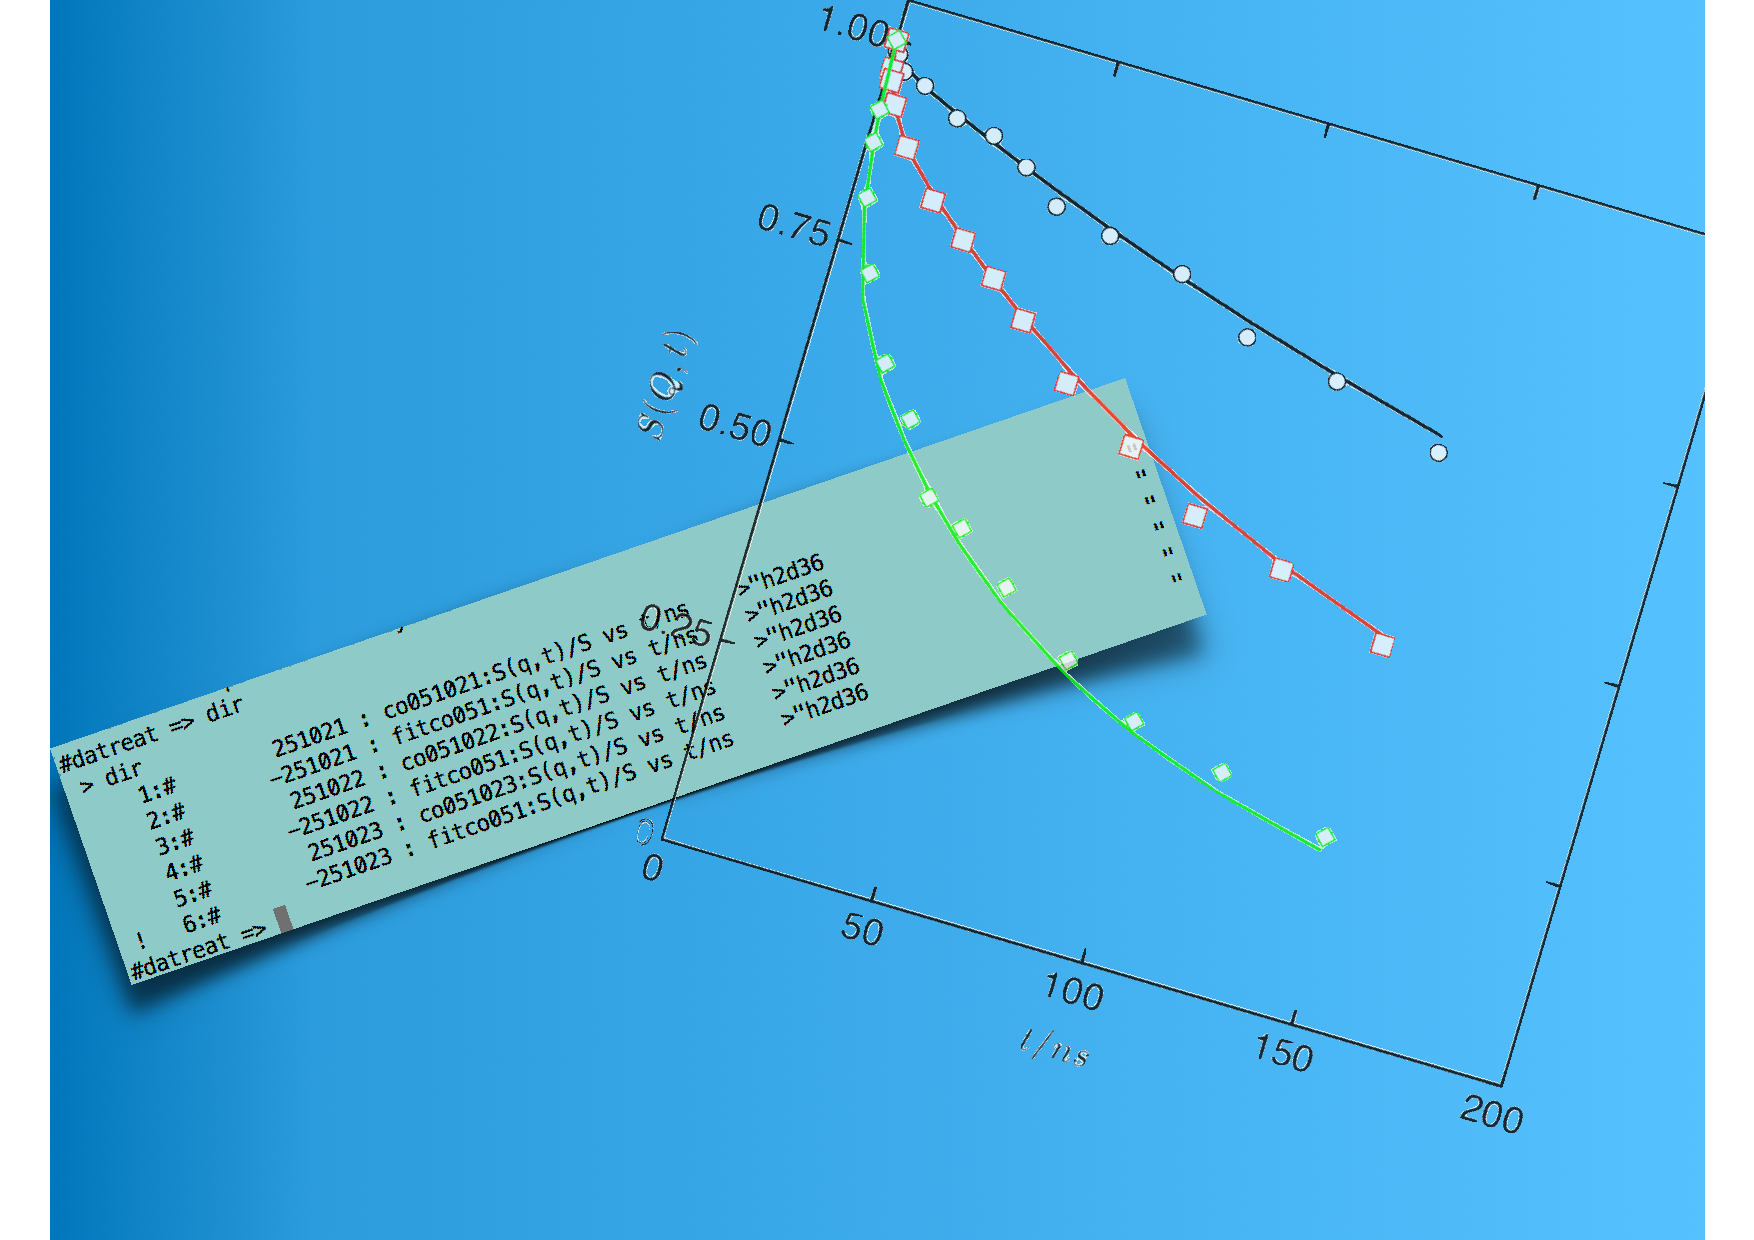
\includegraphics[height=\paperheight]{DatreatLogo.pdf}};
\draw (current page.center) node [fill=ocre!30!white,fill opacity=0.6,text opacity=1,inner sep=1cm]{\Huge\centering\bfseries\sffamily\parbox[c][][t]{\paperwidth}{\centering Datreat Manual\\[15pt] % Book title
{\Large Model fitting and more}\\[20pt] % Subtitle
{\huge Michael Monkenbusch}}}; % Author name
\end{tikzpicture}
\vfill
\endgroup

%----------------------------------------------------------------------------------------
%	COPYRIGHT PAGE
%----------------------------------------------------------------------------------------

\newpage
~\vfill
\thispagestyle{empty}

\noindent Copyright \copyright\ 2019 M.M, Forschungszentrum j\"ulich\\ % Copyright notice

\noindent \textsc{Published by Publisher}\\ % Publisher

\noindent \textsc{book-website.com}\\ % URL

\noindent Licensed under the Creative Commons Attribution-NonCommercial 3.0 Unported License (the ``License''). You may not use this file except in compliance with the License. You may obtain a copy of the License at \url{http://creativecommons.org/licenses/by-nc/3.0}. Unless required by applicable law or agreed to in writing, software distributed under the License is distributed on an \textsc{``as is'' basis, without warranties or conditions of any kind}, either express or implied. See the License for the specific language governing permissions and limitations under the License.\\ % License information, replace this with your own license (if any)

\noindent \textit{First printing, \today } % Printing/edition date

%----------------------------------------------------------------------------------------
%	TABLE OF CONTENTS
%----------------------------------------------------------------------------------------

%\usechapterimagefalse % If you don't want to include a chapter image, use this to toggle images off - it can be enabled later with \usechapterimagetrue

\chapterimage{DatreatLogo.pdf} % Table of contents heading image

\pagestyle{empty} % Disable headers and footers for the following pages

\tableofcontents % Print the table of contents itself

\cleardoublepage % Forces the first chapter to start on an odd page so it's on the right side of the book

\pagestyle{fancy} % Enable headers and footers again

%----------------------------------------------------------------------------------------
%	PART
%----------------------------------------------------------------------------------------

\part{General}

%----------------------------------------------------------------------------------------
%	CHAPTER 1
%----------------------------------------------------------------------------------------

\chapterimage{DatreatLogo.pdf} % Chapter heading image
\chapter{Introduction: read this first!}

\section{Purpose and general modes of use}

\section{Manual \desc{Notation conventions}}
\index{notation}
\index{[..]}

Any input or parts of \enter{input} that is \textbf{literal} is written \enter{like this}. \\
Any input of \var{variable} information/values is written \var{like this}. \\ 
Any \vol{volatile}{} inputs of information/values is written \vol{like}{this}. \\ 
\out{Output} from datreat is written \out{like this}. \\
\textbf{Optional} inputs are indicated \opt{like this}.

\vskip 1cm

\section{Basics of use \desc{data structure and operations}}
% ---------------------
\index{data structure}
\index{record}
\index{operations}
\index{sel}
The data "atoms" (called {\bf records}) are curves/tables of (x,y,y-error) values augmented by
a comment, x- and y-axis labels and a set of parameters that contain  metadata.
Each {\bf record} occupies one slot $j$ in the internal data storage and can be addressed by
this slot number. 
In order to perform some \emph{action} of processing, display etc. the corresponding {\bf records} 
must be {\bf selected}. Depending on the required action  {\bf one or several records} must be
{\bf selected}.
Depending on the performed action the \emph{selection} either is kept or is transferred to
newly created {\bf result records}. This should be mentioned in the execution message issued
by the processing command.
The memory contents and the selection state can be checked using the commands \cmdl{dir}() and/or
\cmdl{dsl}{} (see their description for more detail).
\index{selection}

Fitting requires the specification of a {\bf theory} model, which can be combined form a number
of available models, more advanced modelling can be achieved by adding own models. For details on
model fitting see chapter \emph{Fitting}.

Inspection of {\bf records}, fit results etc. is bets done using the command \cmdl{plot}{}.
\vskip 1cm

\section{The command line \desc{components of the command input}}
%--------------------------
If datreat is ready it shows a prompt: \dtrprompt, then in can be controlled by entering a command line.
Command lines start with a command followed by a number of keywords and values.\\
\index{command line}

\begin{itemize}
\item \cmdl{cmd}{}
\item \cmdl{cmd}{keyword \var{value}}
\item \cmdl{cmd}{option}
\item \cmdl{cmd}{\var{value}}
\item \cmdl{cmd}{\var{value} \var{value} }
\end{itemize}

\vskip 0.5cm


%?% \begin{description}
%?% \begin{}
%?% \item[cmd] command name, it is the first item of the command line
%?% \item[" "] one or several blanks separate any items
%?% \item[Keyword] name like item that serves as identifier for options or following value(s)
%?% \item[Value] Elaboration
%?% \item[\&] command separator allows to enter several command in one line
%?% \end{description}
%?% 
%?% 
%?% \vskip 0.5cm

\begin{tabbing}
\textbf{keyword}  \= command name, it is the first item of the command line                    \kill
\textbf{cmd    }  \> command name, it is the first item of the command line                    \\
\textbf{" "    }  \> one or several blanks separate any items                                  \\
\textbf{keyword}  \> name like item that serves as identifier for options or following value(s)\\
\textbf{Value  }  \> numerical or literal value (depends on keyword)                           \\
\textbf{\&     }  \> command separator allows to enter several command in one line             \\
\end{tabbing}

\begin{corollary}
\cmdl{plot}{xmin \var{x1} xmax \var{x2}}
\end{corollary}

\section{Datreat data structure, variables and built-in functions}
\index{variables}
\index{functions}
\index{user defined}

\begin{tabbing}
\textbf{class xxxxx  }  \= notation xxxxx \= explanation what is its etc.                                 \kill
\textbf{data source  }  \> ${j_s}$    \> index of active source data record                     \\
\textbf{result dest. }  \> ${j_r}$    \> index of resulting data record                         \\
\textbf{selected set }  \> $\cal{S}$  \> set of active source data records (indices)            \\
\textbf{x-values     }  \> $x_j(i)$   \> $i$-th x-value of record $j$                           \\
\textbf{y-values     }  \> $y_j(i)$   \> $i$-th y-value of record $j$                           \\
\textbf{y-errors     }  \> $\delta y_j(i)$   \> $i$-th y-error-value of record $j$             \\
\textbf{parameters   }  \> $p^l_j $   \> $l$-th parameter associated with record $j$            \\
\textbf{variables    }  \> $v^n   $   \> $n$-user defined/system variable/function (global)     \\
\textbf{numor        }  \> $\#     $   \> separate associated id number to each record           \\
\textbf{xname        }  \> ${\text{xname}_j}$ \> x-label (max 80 char) of record $j$            \\
\textbf{yname        }  \> ${\text{yname}_j}$ \> y-label (max 80 char) of record $j$            \\
\end{tabbing}

\noindent
{\bf Internal data representation (example)}

\noindent
\begin{table}[h!]
\footnotesize
%\begin{center}
    \begin{tabular}{ | l | l | l | l | l | l | l |}
    \hline
     record $j$   & name & xname & yname & \#   & $\{p^l_j\}$ & $\{x_j(i), y_j(i), \delta y_j(i) \} $ \\ \hline\hline
     1      & dat1 & q     & s(q)  & 123  & $\{temp_1, conc_1, \cdots\}$ & $\{ i=1,n_1 | q_i, I(q_i), \delta I(q_i) \}$\\ \hline
     2      & dat2 & q     & s(q)  & 124  & $\{temp_2, conc_2, \cdots\}$ & $\{ i=1,n_2 | q_i, I(q_i), \delta I(q_i) \}$\\ \hline
     3      & nse1 & t     & s(q,t)  & 700  & $\{q_3,temp_3,   \cdots\}$ & $\{ i=1,n_3 | t_i, S(q,t_i), \delta S(q,t_i) \}$\\ \hline
     4      & ...  & ...   & ...  & ... & ...  & ... \\ \hline
     ...    & ...  & ...   & ...  & ... & ...  & ... \\ \hline
     nbuf   & xy   & x     & y    & 999 & $\{p1_j, p2_j, \cdots\}$   & $\{ i=1,n_j | x_i, y_i, \delta y_i \}$ \\ \hline

    \hline
    \end{tabular}
%\end{center}
\normalsize
\caption{\label{tab:datastruc}  
Internal representation of data records.}
\end{table}

\begin{tabbing}
\textbf{keyword--}  \= command name, it is the first item of the command line                    \kill
\textbf{record j }  \> actual sequence number (address) of one ${(y,y,\delta y)}$ table including metadata  \\
\textbf{name     }  \> short (max. 8 characters) name-id of that table                                      \\
\textbf{xname    }  \> label of x-axis (max. 80 characters) ,it may contain latex elements if it starts with "\$\$" \\
\textbf{yname    }  \> label of y-axis (max. 80 characters) ,it may contain latex elements if it starts with "\$\$" \\
\textbf{\#       }  \> numeric id code (numor), mostly for information only                                 \\
\textbf{$p_j^l$  }  \> metadata, l-th parameter (\textbf{name(8)}, {\it value}) of this, $j$, record            \\
\textbf{$\{x_j(i),\cdots\}$}  \> $n_j$ table values ${(y,y,\delta y)}$             \\
\end{tabbing}

\subsection{Variables and functions \desc{user defined variables, datreat variables and functions}}
% ----------------------------------------------------------------------------------------
\index{variables}
\index{functions}
\index{expression, variables and functions}
With the \cmdl{set}{} command one can create and modify (floating point) variables that can be
referred in expressions, commands and input.

{\bf Note:} Defining a \emph{user variable} with the same name as a \emph{parameter} of a data record
makes the parameter invisible, all references in expressions yield the value of the defined \emph{user variable}
until it is removed by \cmdl{clr}{varname}.

\subsection{Global functions}

\linespace
\textbf{Mathematical functions}
\linespace
\begin{tabbing}
\textbf{keyword--}  \= command name, it is the first item of the command line                    \kill
\textbf{sin(..)  } \>  $\sin(x)  $  std sine            \\         
\textbf{cos(..)  } \>  $\cos(x)  $  std cosine          \\
\textbf{tan(..)  } \>  $\tan(x)  $  std tan             \\
\textbf{atan(..) } \>  $\arctan(x) $  std arctan          \\
\textbf{asin(..) } \>  $\arcsin(x) $  std arcsin          \\
\textbf{acos(..) } \>  $\arccos(x) $  std arccos          \\
\textbf{ln(..)   } \>  $\ln(x)   $  std natural log     \\
\textbf{exp(..)  } \>  $\exp(x)  $  std exp             \\
\textbf{sqrt(..) } \>  $\sqrt{x} $  std square root     \\
\textbf{abs(..)  } \>  $|x|  $  std absolute value  \\
\textbf{int(..)  } \>  $floor(x)  $  std integer         \\     
\textbf{erf(..)  } \>  $\rm erf(x)  $  error function       \\     
\textbf{J0(..)   } \>   Bessel function ${J_0(x)}$       \\     
\textbf{J1(..)   } \>   Bessel function ${J_1(x)}$           
\end{tabbing}

\linespace
\color{blue}
\textbf{Datreat functions and variables}
\index{functions and variables in datreat}
\index{value extraction}
\index{theory parameter extraction}
\linespace
\begin{tabbing}
\textbf{keyword---------}  \= command name, it is the first item of the command line                    \kill
\textbf{X       } \>  the actual x-value implicitly runs over (j,i) in actions on records (note: capital letter!)   \\  
\textbf{Y       } \>  the actual y-value  "        \\  
\textbf{ERR     } \>  the actual y-value  "       \\  
\textbf{x       } \>  the actual x-value (same as X but will be kept in axis name as x)        \\  
\textbf{y       } \>  the actual y-value (same as Y but will be kept in axis name as y)         \\  
\textbf{err     } \>  the actual y-value (same as ERR) "       \\ 
 \\
\textbf{nbuf    } \>  total number of records in memory           \\  
\textbf{nsel    } \>  total number of \textbf{selected} records          \\  
\textbf{sel     } \>  address j of the \textbf{first} selected record            \\  
\textbf{maxx    } \>  maximum x-value of the first selected record            \\  
\textbf{minx    } \>  minimum x-value of the first selected record            \\  
\textbf{maxy    } \>  maximum y-value of the first selected record            \\  
\textbf{miny    } \>  minimum y-value of the first selected record {\color{green}{TBD:all sel recs}}           \\  \textbf{MAXX    } \>  maximum x-value of all selected records            \\  
\textbf{MINX    } \>  minimum x-value of all selected records            \\  
\textbf{MAXY    } \>  maximum y-value of all selected records            \\  
\textbf{MINY    } \>  minimum y-value of all selected records {\color{green}{TBD:all sel recs}}           \\  
\textbf{centerx } \>  "center of mass" of first selected record using data from present fit range only  \\  
\textbf{widthxx } \>  width obtained for the distribution around centerx \\  
\\
\textbf{xv(j,i)  } \>  i-th x-value of record j  (requires no selection)            \\         
\textbf{yv(j,i)  } \>  i-th y-value of record j  (requires no selection)            \\         
\textbf{ye(j,i)  } \>  i-th y-error of record j  (requires no selection)            \\ 
\textbf{nv(j)    } \>  number of table points in record j                           \\ 
\\
\textbf{indxval(j,x)}   \>  point index i (float) of x-value = x in record j        \\ 
\textbf{intxval(j,x)}   \>  point index i (integer) of x-value = x in record j      \\ 
\textbf{sumx(j,l,m)}    \>  sum of x-values l$\cdots$m of record j :${\sum_{i=l}^{m} y_j(i)}$ \\ 
\textbf{sumy(j,l,m)}    \>  sum of y-values l$\cdots$m of record j :${\sum_{i=l}^{m} y_j(i)}$ \\ 
\textbf{sumyerr(j,l,m)} \>  error of sum of y-values l$\cdots$m of record j :${\sum_{i=l}^{m} y_j(i)}$ \\ 
\\
\textbf{isel(n)  } \>  address j of the n-th selected record \\ 
\\
\textbf{num(j) } \>  id-number (numor) of record at address j                       \\ 
\textbf{sc(num)} \>  record address j with id-number=numor (first occurance)           \\ 
 \\
\textbf{th\_par(ip,it)}  \>  value of the ip-th parameter of the it-th activated theory    \\ 
\textbf{th\_err(ip,it)}  \>  error for th\_par    \\ 
  \\
\textbf{om(j,i)}  \>  frequency of the TOF data in point i of record j (requires TOF parameters)   \\ 
\textbf{en(j,i)}  \>  frequency of the TOF data in point i of record j (requires TOF parameters)    \\ 
        
\end{tabbing}
\color{black}


\subsection{Expressions}
\index{expressions}
The notion \textbf{expression} is used for parts of input/command lines that are to be converted
to numerical values upon reading. The simplest \textbf{expression} is just a numerical value.
Genuine expressions are arithmetic expression that can contain functions, user defined variables and
datreat specific global functions and variables.
\linespace
Genuine expressions must be given in \textbf{brackets (...) } and may not contain any blanks!
\linespace
A fast check to what value an expression will evaluate one can us the command \cmdl{??}{expression}
\index{expressions}

An expression can occur at any place, where a numerical input is expected.
\linespace
{\bf Examples:}
\begin{corollary}
% \sysprompt \enter{cd \emph{Myworkingdirectory}} \return \\
\dtrprompt \cmdl{set}{myvar1 \var{1.23}}       \return \\
\dtrprompt \cmdl{set}{myvar2 \var{0.77}}       \return \\
\dtrprompt \cmdl{??}{(exp(-myvar1+3*myvar2))}  \return \\
\out{> ?? (exp(-myvar1+3*myvar2))} \\
\out{  2.9446795510655241}    
\end{corollary}



\section{Customisation (Makros) \desc{How to combine commands}}
\index{makros}
Sometimes one notices that complex commands or command sequences have to be repeated
frequently. To save typing and increase the efficiency of \emph{datreat} usage \textbf{makros}
can be used.
This may start with just associating another name to a command (for better memorisation) to
more complex constructions with conditions and loops etc.
 
\linespace
Makros are simple text-files that contain a sequence of datreat commands or other makro calls.
The only special syntax rules pertain the {\bf first line} of the makro, which looks like this:

\begin{corollary}
% \sysprompt \enter{cd \emph{Myworkingdirectory}} \return \\
\bf 
makro       \return \\
makro \_arg1\_ \      \return \\
makro \_arg1\_ \_arg2\_ $\cdots$       \return 
\end{corollary}
\index{arguments (makro)}

The keyword {\bf makro} is necessary to confirm to \emph{datreat} that this file is a makro.
Optionally one or several arguments: {\bf \_arg1\_ \_arg2\_  $\cdots$} can be present.

A simple example is a makro {\bf pstyle} that plots selected records of NSE data in publication 
ready style:

\begin{corollary}
makro                                                       \\
rename yaxis \$\$S(Q,t)                                     \\ 
rename xaxis \$\$t\/ns                                      \\
plot ymax 1.05 txoff flinewd 1.2 axtxsize 1.3 xlegdist 0.1  
\end{corollary}

Or slightly more complex a makro with one argument (here a filename) that reads the
record table content of saved data \cmdl{in}{filename} and then tries to extract theory 
\cmdl{get\_th}{filename}. The filename of the makro, i.e. the makro name is {\bf inplus},
its contents:

\begin{corollary}
makro  \_f\_
! input file (as created by msave) and activate the theory definition contained
in     \_f\_
get\_th \_f\_
\end{corollary}
the filename variable \emph{\_f\_} is inserted into the command lines present in the makro by
{\bf string replacement}. Lines starting with {\bf !} are comments and ignored by \emph{datreat}.

To use the makro in datreat:
\begin{corollary}
% \sysprompt \enter{cd \emph{Myworkingdirectory}} \return \\
\dtrprompt \cmdl{inplus}{myMsavedData}       \return 
\end{corollary}

For the system to be able to find a makro it should either be {\bf stored in the current working
directory}, such that it is strictly associated to the evaluation done with the data there.
Or it may be put to the standard makro directory (\emph{datreat/makros/...}, then it should be
visible for any \emph{datreat} instance. Makros in the current working directory will mask
those with the same name in the standard makro directory.  

{\bf Note:} Makros with names that match genuine \emph{datreat} command names will not be recognized.
\subsection{Makros specific commands}

\linespace
\begin{tabbing}
\textbf{keyword----------------------------------------------}  \= xxxxxxxxxxxx  \kill
\cmdl{!}{}           \>  line content from here is comment only          \\         
\cmdl{:lab}{}        \>  label, the rest of the line is ignored          \\         
\cmdl{say}{message}  \>  display (speak) a message         \\         
\cmdl{if}{(expr1) <= (expr2) then goto :lab}  \>  conditional jump to label :lab         \\         
\cmdl{goto}{:lab}    \>  unconditional jump to label :lab         \\         
\end{tabbing}


\section{Necessary and useful UNIX commands (Mac)}
\index{UNIX}
\index{MAC-OS}
\index{cd, unix change directory}
\index{cp, unix file copy}
\index{mv, unix file move (rename)}
\index{rm, unix file remove}
\index{cat, unix file content}
\index{$>$, unix redirection}
\index{$>>$, unix redirection}
\index{$<$, unix redirection}
\begin{tabbing}
\textbf{keyword--} \= -------------------------------------------  \= xxxxxxxxxxxx  \kill
\textbf{cd} \> \emph{directory}  \> change directory                 \\
\textbf{ls -ltr} \>             \> list files in directory          \\
\textbf{pwd}  \>                \> show the current directory path  \\
\textbf{cp} \> \emph{file1} \emph{file2}   \> copy file1 to file2    \\
\textbf{mv} \>  \emph{file1} \emph{file2}   \> move/rename file1 to file2  \\
\textbf{rm} \>  \emph{file1}                \> remove file1 (delete)  \\
\textbf{cat} \>  \emph{file1}               \> lists file content  \\
{$\bf{ >}$}  \>  \emph{cmd $>$ file1}           \> redirection: writes output of cmd to file1  \\
{$\bf{ >>}$} \>  \emph{cmd $>>$ file1}           \> redirection: APPENDS output of cmd to file1  \\
{$\bf{ <}$}  \>  \emph{cmd $<$ file1}           \> redirection: inputs contents of file1 to cmd  \\
{$\bf{ |}$}   \> \emph{cmd1 $|$ cmd2}           \> pipe: output of cmd1 is used as input for cmd2  \\
\end{tabbing}

{\bf Note:} File operations on this level cannot be undone!
% ----------------------------------------------------------------------------------------
\chapterimage{DatreatLogo.pdf} % Chapter heading image
\chapter{First steps}
%------------------------------------------------------------
\section{Starting and quitting the program}
%--------------------------------
\index{starting datreat}
After installation according to the procedure described in \ref{sec:install} the program should be
ready to use. This is done by opening a \textbf{terminal} and change the directory to where the
work shall be performed. Then start \textbf{datreat} by typing \emph{datreat \return}.

%\begin{mdframed}[linecolor=gray,linewidth=2pt,leftmargin=2cm,rightmargin=2cm,backgroundcolor=lightgray] 
%\sysprompt cd Myworkingdirectory \return \\
%\sysprompt datreat \return \\
%\dtrprompt 
%\end{mdframed}

\begin{corollary}
\sysprompt \enter{mkdir \emph{Myworkingdirectory}} \return \\
\sysprompt \enter{cd \emph{Myworkingdirectory}} \return \\
\sysprompt \enter{datreat }\return 
\dtrprompt
\end{corollary}

\index{quit}
\index{exit}
After use \emph{datreat} by be exited by the commands:
\begin{corollary}
\dtrprompt \enter{quit} \expl{Leaves datreat and saves last state} \\
or \\
\dtrprompt \enter{exit} \expl{Leaves datreat WITHOUT saving} 
\end{corollary}

\linespace

{\bf Note 1:}
\begin{corollary}
\sysprompt \enter{datreat 0} \expl{Starts datreat without restoring the last state} 
\end{corollary}
However, the last plot setting is kept. Remove file
\emph{last\_plotsetting} to return back to default prior 
(re)start of datreat.

\linespace

{\bf Note 2:}
The last state is stored in the following files:
\begin{itemize}
    \item last\_datreat\_content \expl{data records}
    \item lastselections \expl{actual selections, requires unique nonzero numors !}
    \item lastusv \expl{uservariable with contents}
    \item lastth \expl{theory settings}
    \item last\_plotsetting \expl{plot settings, always kept}
\end{itemize}
These settings are stored in the current working directory and therfore are "private" to that topic. Treating another problem in another working directory will have its own last-state.

\linespace

{\bf Note:} It is recommended to do the work on one topic in a dedicated \emph{subdirectory},
which the will contain the comment history, the last state of the program and any plots or
other output. The used data may be copied to that \emph{subdirectory} or addressed by using
the full path specification (see also the {\bf path} command).

%\begin{theorem}
%cd Myworkingdirectory \\
%datreat 
%\end{theorem}

\part{Input, records and display}

\chapterimage{DatreatLogo.pdf} % Chapter heading image
\chapter{Data management I/O}
%-------------------------------------------------------------------------------------------------------------
\section{input \var{filename} \desc{input files and data format}}
\index{input of data from files}
\index{format (input files)}
\index{path (input files)}
Synonym: {\bf in}
\linespace
Reading data from ASCII files that may contain a header of metadata followed by a table containing the
proper (x, y) data with an optional 3rd column with y-errors. The data are read into datreat memory, each
(x, y)-table group is represented by one {\bf record}, the record addresses $j$ are filled in the sequence
of reading. File names can be arbitrary, except that a few extensions indicate special deviating data formats 
(e.g. inx or ins). 
 
The default \emph{subdirectory} (i.e. \emph{path}) where input files are expected is the
\emph{current working directory}. This may be changed either by explicitly specifying
a path in front of the filename in the {\bf input command} or by using:

\begin{corollary}
\dtrprompt \cmdl{path}{} \expl{lists paths setting in this session}  \return \\ 
\dtrprompt \cmdl{datapath}{\var{PATH-TO-DATA}} \expl{sets data-path for this session}  \return 
\end{corollary}

\begin{corollary}
\dtrprompt \cmdl{in}{\var{filename}}  \return 
\end{corollary}

{\bf Note:}After \cmdl{in}{} ALL records with \emph{positive numor} (i.e. omitting fit results) 
that have been read are \emph{SELECTED}!


\section{dir \opt{pname} \desc{listing data holding records}}
\index{listing loaded files}
\index{display memory content (records)}


Displays the present contents of the \emph{datreat} memory in terms of a list of loaded records.

\begin{corollary}
\dtrprompt \cmdl{dir}{\var{parname1, parname2, ...}}  \return 
\end{corollary}

\linespace
{\bf Example:}
\begin{corollary}
% \sysprompt \enter{cd \emph{Myworkingdirectory}} \return \\
\dtrprompt dir  q  temp              \return \\
\color{blue}
\footnotesize
\begin{verbatim}
 > dir q temp
   1:#  974101 : 6SB520 :fqt  vs t/ns  >"6SB520C 6SB5 2mm "  q   0.041468 temp  295.29         
   2:#  974103 : 6SB520 :fqt  vs t/ns  >"6SB520C 6SB5 2mm "  q   0.058920 temp  295.29         
   3:#  974104 : 6SB520 :fqt  vs t/ns  >"6SB520C 6SB5 2mm "  q   0.082602 temp  295.29         
!  4:#  974105 : 6SB520 :fqt  vs t/ns  >"6SB520C 6SB5 2mm "  q   0.098593 temp  295.29         
!  5:#  974106 : 6SB520 :fqt  vs t/ns  >"6SB520C 6SB5 2mm "  q   0.122080 temp  295.29         
!  6:#  974107 : 6SB520 :fqt  vs t/ns  >"6SB520C 6SB5 2mm "  q   0.137806 temp  295.29         
!  7:#  974110 : 6SB520 :fqt  vs t/ns  >"6SB520C 6SB5 2mm "  q   0.157455 temp  295.29         
!  8:#  974112 : 6SB520 :fqt  vs t/ns  >"6SB520C 6SB5 2mm "  q   0.179635 temp  295.29       
\end{verbatim}
\color{black}
\normalsize
\end{corollary}
The example output contains the following information:
\index{ !  (dir)}
\index{\#  (dir)}
\index{vs  (dir)}

\begin{tabbing}
column \= \textbf{keyword----}   \= command name, it is the first item of the command lin            \kill
column \> example \> description \\
1  \> \textbf{!        }     \> an exclamation mark in column 1 indicates that the record is {\bf selected}  \\
2  \> \textbf{1:, 2: ..}     \> record address $j$                                                           \\
3  \> \textbf{\# 97$\cdots$}  \> numeric-id (numor) of this record (mainly information)                       \\
4  \> \textbf{6SB520  }      \> name-id                                                                      \\
5  \> \textbf{fqt     }      \> y-axis name                                                                  \\
6  \> \textbf{vs     }       \> fix keyword (versus)                                                         \\
7  \> \textbf{$>$".."}       \> first n-characters of the record {\bf comment}                               \\
8  \> \textbf{q}             \> name of first specified parameter to be listed (volatile option)             \\
9  \> \textbf{0.04$\cdots$}  \> value of parameter $q$ for this record                                       \\
10 \> \textbf{temp}          \> name of 2nd specified parameter to be listed (volatile option)                \\
11 \> \textbf{295$\cdots$}   \> value of parameter $temp$ for this record                                      
\end{tabbing}

\section{purge \opt{all|rest|sel}}
Removes all {\bf selected} or \emph{all} data from the record address list.
Or \emph{rest} = all not selected records.
\index{purge}
\index{clearing records}
\index{deleting records}


\begin{corollary}
\sysprompt \cmdl{purge}{rest} \return  \expl{clear record memory but keeps selected records} \\
\sysprompt \cmdl{purge}{all}  \return  \expl{clear record memory completely} \\
\sysprompt \cmdl{purge}{sel}  \return  \expl{removes all selected records}
\sysprompt \cmdl{purge}{fits} \return  \expl{removes all fits/calculated records (those with negative numor}
\end{corollary}
Clear the stored record list.

\linespace

{\bf Note:} Record addresses may (will) change if some are removed. 

\section{msave \var{filename} \desc{save data and fit results}}
Save all selected records (including fitted/computed curves) and the currently active
theory model to file \var{filename}
\index{msave}
\index{saving results and parameters on a file}

\begin{corollary}
\sysprompt \cmdl{msave}{filename}  \return 
\end{corollary}

\tbd{consolidate plotting actions by this... title setting etc.  }


\section{inplus \var{filename} \desc{read msave-stored data with theory model}}
\index{inplus}
\index{msave (read stored data)}
Read records that have been save by \cmdl{msave}{} including the stored active
theory model from file \var{filename}.

{\bf Note:}The record addresses will most probably different form those when stored!
{\bf Note:}Any actual theory model definition will be replaced by that store in file \var{filename}.

\begin{corollary}
\sysprompt \cmdl{inplus}{filename}  \return 
\end{corollary}

\index{restore saved content}

\tbd{make it a genuine command }


\section{putpar \desc{adding/setting data-record associated parameters}}
\index{putpar}
\index{record parameter}
\index{fitting multiple records discriminated by parameters}

\begin{exercise}
Add a new parameter (with value) or change value of record associated parameters in {\bf all 
selected records}.
Ideally with \emph{input} all relevant parameter associated with the respective data record
should also be read-in by the \emph{input} command.
Often, however, this is not the case and additional information needed by some \emph{theories}
or as plain information in plot legends or for selecting a subset of loaded records are still
missing. The {\bf putpar} offers a means to add this information.
\end{exercise}

\begin{corollary}
% \sysprompt \enter{cd \emph{Myworkingdirectory}} \return \\
\dtrprompt \cmdl{sel}{ \emph{selection list}} \expl{first select the records to be affected}  \return \\
\dtrprompt \cmdl{putpar}{ \var{parname} \var{value} } \expl{assign \var value to parname}   \return  
\end{corollary}

\linespace

{\bf Example:}
\begin{corollary}
% \sysprompt \enter{cd \emph{Myworkingdirectory}} \return \\
\dtrprompt  sel 1 2 3         \return  \expl{select records 1 and 2 and 3} \\
\dtrprompt  putpar temp 373   \return  \expl{set/create parameter \emph{temp} to value 373} 
\end{corollary}


{\bf Note1:} In the present version of datreat the name \emph{parname} has a length limit
of 8 characters. 
 
{\bf Note2:} The parameters are displayed in the plot legend. 

{\bf Note3:} The parameters can be inspected by {\bf dir \var{parname1} \var{parname2} $\cdots$ } or for
selected records only by {\bf dsl \var{parname1} \var{parname2} $\cdots$ }.

{\bf Note4:} The parameters may be used in selection criteria by   
{\bf sel all \var{parname} \var{value} band \var{value} } 

\begin{exercise}
{\bf Attention!}  In order to preserve the added parameter information select all
relevant records and store a copy using the {\bf msave \var{newname}} command.
And restore it using {\bf input \var{newname}} or  {\bf inplus \var{newname}}.
\end{exercise}

{\bf Note5:} The value of a parameter assoiated with the {\bf first} selected record
can be addressed in any expressions by {\bf (\var{parname})} that is evaluated to 
the parameter value.

{\bf Note6:} Of course parameters can (permanently) be added to record data files by
directly editing and adding lines to the parameter section in the beginning of the
data files.


\section{copy \desc{copy records in memory}}
\index{copy records}
\index{duplicate records}
Copy \emph{selected} records to the end of the record list (selection moves to copy).

\begin{corollary}
\sysprompt \cmdl{copy}{}  \return \expl{copy selected records}
\end{corollary}



\section{allsave \desc{save current datreat state to subdirectory}}
\index{save state}
\index{store}
Copy all information needed to restore currently loaded data, theories, selection, plotsettings etc . 
to a subdirectory.This is a \emph{makro}.

\begin{corollary}
\sysprompt \cmdl{allsave}{DIRNAME}  \return \expl{copy present state to subdir DIRNAME}
\end{corollary}

{\bf Note:}Use (makro) \emph{allresto} to restore!


\section{allresto \desc{restore cdatreat state from a subdirectory}}
\index{restqore state}
\index{restore}
Restore datreat state (loaded data, theories, selection, plotsettings etc . )
from a subdirectory.This is a \emph{makro}.

\begin{corollary}
\sysprompt \cmdl{allresto}{DIRNAME}  \return \expl{restore state from subdir DIRNAME}
\end{corollary}

{\bf Note:}Use (makro) \emph{allsave} to save state!


\chapterimage{DatreatLogo.pdf} % Chapter heading image
\chapter{Select}
%-------------------------------------------------------------------------------------------------------------
\index{selecting records for actions}
Selection of records is the way to control on which data the following command actions are to be
applied. The main command \cmdl{sel}{} besides the plain selection according to record address $j$
a number of powerful options.
\linespace
{\bf Note:} The sequence of selection matters!
\linespace

\section{sel \opt{spec} \desc{select data records for next actions}}
\index{sel}
\index{selection (for next actions)}
\index{target records}
There are a number of methods to select records. Since selection is a genuine to control the 
evaluation in \emph{datreat} in the following the methods (\opt{spec}) are explained one by one.

\begin{corollary}
\dtrprompt \cmdl{sel}{ ${j_1 \; j_2 \; j_3 \cdots}$ }  \return 
\end{corollary}
Selects record addresses $j_1$, $j_2$, etc..

\linespace


\begin{corollary}
\dtrprompt \cmdl{sel}{ ${j_1 \; -j_2}$ }  \return 
\end{corollary}
Selects a continuous range of record addresses $j_1 \cdots j_2$,
note ${-j_2}$ means the negative of the address, i.e. no blank between "-" and the
address value is allowed.
\linespace


\begin{corollary}
\dtrprompt \cmdl{sel}{ ${j_1 \; -j_2  \; -j_s}$ }  \return \expl{e.g. select all odd or even addresses in range ...}
\end{corollary}
Selects a continuous range of record addresses $j_1 \, , \, j_1+j_s , \, j_1+2 j_s \, \cdots j_2$,
note ${-j_2}$ means the negative of the address, i.e. no blank between "-" and the
address value is allowed. A further negative number $-j_s$ allows to specify a step between
the address selection in the continuous range between $j_1$ and $j_2$. This allows, e.g.
the simple selection of all odd or all even addresses etc..

\linespace

\begin{corollary}
\dtrprompt \cmdl{sel}{add ${j_1 \; j_2 \; j_3 \cdots}$  }  \return 
\end{corollary}
Appends record addresses $j_1$, $j_2$, etc.. to the current selection list.

\linespace


\begin{corollary}
\dtrprompt \cmdl{sel}{${j_1 \; j_2 \; j_3 \cdots}$ fit+  \return \expl{selects records including fitted curves} }  
\end{corollary}
Selects ${j_1 \; j_2 \; j_3 \cdots}$ and 
associate corresponding fitted curves to the selection.
{\bf Note:} this is automatically done by the fitting process but is lost by following
\cmdl{sel}{} commands.

\linespace

\begin{corollary}
\dtrprompt \cmdl{sel}{next \it parname ${p}$ \rm band \it ${\Delta p}$   }  \return 
\end{corollary}
Selects the next (scanning record addresses starting form the last selected record)
that has a parameter \var{parname} with value equal to ${p\pm \Delta p}$.

\linespace

\begin{corollary}
\dtrprompt \cmdl{sel}{all \it parname ${p}$ \rm band \it ${\Delta p}$   }  \return 
\end{corollary}
Selects all records that have a parameter \var{parname} with value equal to ${p\pm \Delta p}$.

\linespace

\begin{corollary}
\dtrprompt \cmdl{sel}{narrow \it parname ${p}$ \rm band \it ${\Delta p}$   }  \return 
\end{corollary}
Selects all records form the currently selected list 
that have a parameter \var{parname} with value equal to ${p\pm \Delta p}$.

\linespace

\begin{corollary}
\dtrprompt \cmdl{sel}{exclude \it parname ${p}$ \rm band \it ${\Delta p}$   }  \return 
\end{corollary}
Remove all records form the currently select list 
that have a parameter \var{parname} with value equal to ${p\pm \Delta p}$.

\linespace

\begin{corollary}
\dtrprompt \cmdl{sel}{exclude numor mod \it m   }  \return 
\end{corollary}
Remove all records form the currently select list 
that have a numeric-id parameter numor ${N}$ that matches ${\mod (N,m)=0}$.

\linespace

\begin{corollary}
\dtrprompt \cmdl{sel}{}  \return 
\end{corollary}
removes all selections.

\linespace


\section{dsl \desc{display list of selected records}}
Display a list of the selected records (similar to \cmdl{dir}{} but restricted to selected records.
end{corollary}
\index{list selected records}
\index{display selected records}

\begin{corollary}
\dtrprompt \cmdl{dsl}{\var{parname1, parname2, ...}}  \return 
\end{corollary}

\linespace
{\bf Example:}
\begin{corollary}
% \sysprompt \enter{cd \emph{Myworkingdirectory}} \return \\
\dtrprompt dsl  q  temp              \return \\
\color{blue}
\footnotesize
\begin{verbatim}
 > dsl q temp
3 [ 0]:# 974104 : _6SB5_20:t/ns vs fqt  >"_6SB5_20C _6SB5 2mm " q 0.082602 temp 295.29          
4 [ 0]:# 974105 : _6SB5_20:t/ns vs fqt  >"_6SB5_20C _6SB5 2mm " q 0.098593 temp 295.29          
5 [ 0]:# 974106 : _6SB5_20:t/ns vs fqt  >"_6SB5_20C _6SB5 2mm " q 0.122080 temp 295.29          
\end{verbatim}
\color{black}
\normalsize
\end{corollary}
In analogy to the dir command, in [brackets] the addresses of the associated fitted curve 
records are shown (0=no fit associated).



\section{activate \desc{theory model activation}}
\index{theory define (activate)}
\index{activate a theory}
\index{model definition}
Activate (synonym {\bf ac} is used to set up a model assembled from the current collection of
available theories. The \emph{activated} model may the be fitted or compared by calculation with
data records.

A list of available theories (names only) is obtained by the command \cmdl{th}{}.
More information on one of these theories can be displayed using
\begin{corollary}
% \sysprompt \enter{cd \emph{Myworkingdirectory}} \return \\
\dtrprompt \cmdl{th}{theoryname}  \return 
\end{corollary}

\linespace
The (fit)-model can then be assembled by single or multiple activation commands:
\begin{corollary}
\dtrprompt \cmdl{ac}{\var{theoryname1}}  \return 
\dtrprompt \cmdl{ac}{\var{theoryname2}}  \return 
\dtrprompt \cmdl{ac}{$\cdots$}     \return 
\end{corollary}
The results of the thus \emph{activated} theories are {\it added} to yield the final result.
\begin{corollary}
\dtrprompt \cmdl{ac}{\var{theoryname3} multiply}  \return 
\end{corollary}
will add a further definition the result of which will be multiplied to the result of the
precedent activated theories. {\bf Note:} starting with a \emph{multiplied} theory is nonsense.
\begin{corollary}
\dtrprompt \cmdl{ac}{\var{theoryname} range \var{parname} min \var{value1} max \var{value2} }  \return 
\end{corollary}
Causes that instance of the theory only to be evaluated if the value of the parameter /var{parname}
of the record under actual comparison lies within the ${min \cdots max}$ range.  

\linespace
To {\bf set the parameters} of the activate theory model use \cmdl{cth}{}, which opens an editor
that allows to set numbers or otherwise modify the model, choose which parameters shall be fitted and
possibly establish parameter couplings (see. sec....).

{\bf Note:} The actual theory model definition as e.g. modified using \cmdl{cth}{} is always stored
on file \emph{lastth} in the current working directory. It also will be appended to the file written
by \cmdl{msave}{filename}.

\begin{corollary}
\dtrprompt \cmdl{al}{} \return 
\end{corollary}
displays the actually loaded theory model (normally this is implicitly executed upon loading/modifying).


\section{acl \desc{Loading previous theory model}}
\index{load previous theory definition}
\begin{corollary}
\dtrprompt \cmdl{acl}{} \return 
\end{corollary}
loads the last theory model, which is on file \emph{lastth}. {\bf Note:} \emph{lastth} is updated each time
a theory model is update or modified, i.e. by fitting.


%% --------------------------------------------------------------------------------------------------------------
\chapterimage{DatreatLogoPlt.pdf} % Chapter heading image
\chapter{Data inspection and plotting}
\index{display data}
\index{plot}

\section{plot \desc{basic data display}}
Plotting of the \emph{selected} records and (if present) associated fitted curves. 

\begin{corollary}
\dtrprompt \cmdl{plot}{}  \return 
\end{corollary}
Plots the selected records using the current axis and style settings.

\linespace

\begin{corollary}
\dtrprompt \cmdl{plot}{xmin \var{xmin}  xmax \var{xmax}  ymin \var{ymin}  ymax \var{ymax} }  \return 
\end{corollary}
Plots the selected records after setting the x- and/or y- limits.
{\bf Note:}
\begin{corollary}
\dtrprompt \cmdl{plot}{xmin (minx) xmax (maxx) ymin (miny) ymax (maxy)  }  \return 
\end{corollary}
Realizes and auto scaled plot.

\linespace
\index{plot (lin, log axes)}

\begin{corollary}
\dtrprompt \cmdl{plot}{log\_x log\_y}  \return 
\end{corollary}
Plots the selected records using log-scaled axes (either x or y or both). 

\linespace

\begin{corollary}
\dtrprompt \cmdl{plot}{lin\_x lin\_y}  \return 
\end{corollary}
Plots the selected records using (back to normal) lin-scaled axes (either x or y or both). 

\linespace

\index{plot (comparing curves with individual scales)}
\begin{corollary}
\dtrprompt \cmdl{plot}{scaled \var{f1} \var{f2} $\cdots$ }  \return 
\end{corollary}
Plots after scaling the $N$ selected records (in the sequence of selection) by factors ${f_1 \cdots f_N}$.
The scaling factors are reported in the legend part of the plot. {\bf Note:} {\bf scaled} is a 
volatile option. It has to be specified each time when is shall be applied. The selected records are
not changed.

\linespace

\index{plot (clipping)}
\begin{corollary}
\dtrprompt \cmdl{plot}{clip}  \return 
\end{corollary}
Plots with exact clipping of curves.
{\bf Note:} {\bf clip} is a 
volatile option. It has to be specified each time when is shall be applied. The selected records are
not changed.

\linespace

\section{plot (styling) \desc{Sizes, colors and legends}}
\index{plot (style)}
\index{plot (letter and symbol sizes)}
\index{plot (colors)}
\index{plot (legends)}
\index{plot (publication ready)}
To yield publication style plots or make things better visible there are a number of style modification
options.

\begin{corollary}
\dtrprompt \cmdl{plot}{sysize \var{sz}  symb \var{S1} \var{s2} $\cdots$ }  \return 
\end{corollary}
Plots the selected records using symbols with numbers \var{S1}, \var{S2} $\cdots$ assigned in the
sequence of selection. Symbol type number 0 yields a line.
\var{sz} is (global) symbol size scaling (default is 0.7).
Symbol types are: 
{\bf 0:line, 
1:dots, 
2:open circles, 
3:open squares, 
4:open diamonds, 
5:triangle\_up,
6: triangle\_down, 
7:diabolo, 
8:solid\_triangle\_up, 
9:solid\_triangle\_down, 
10:solid\_square, 
11:plus, 
12:star, 
13:cross,
14:solid\_circle, 
15:solid\_diabolo, 
16:hourglass, 
17:solid hourglass,
18:solid diamond, 
19:star2, 
20:solid star2, ...}.

\linespace

\begin{corollary}
\dtrprompt \cmdl{plot}{lwid \var{lw1} \var{lw2} ... ltype \var{lt1} \var{lt2} ...   }  \return 
\end{corollary}
Plots the selected records using line widths \var{lw1}, ... and line types \var{lt1} ... .
Line types are: {\bf 1:solid, 2:dashed, 3:dotted, 4, 5, ...:dash-dotted}.

\linespace

\begin{corollary}
\dtrprompt \cmdl{plot}{colo \var{C1} \var{C2} $\cdots$ }  \return 
\end{corollary}
Plots the selected records using colors with numbers \var{C1}, \var{C2} $\cdots$ assigned in the
sequence of selection.
Colors are: {\bf 0:black, 1:red,  2:green, 3:blue, 4:cyan, 5:yellow, 6:magenta, 7:black, ...}.


\linespace

\begin{corollary}
\dtrprompt \cmdl{plot}{errors | noerrors}  \return 
\end{corollary}
Plots the selected records including error bars ({\bf errors}) or without error bars ({\bf noerrors}).


\linespace

\begin{corollary}
\dtrprompt \cmdl{plot}{parplo | noparplo [\var{pn1} \var{pn2} ...]}  \return 
\end{corollary}
Plot with all record parameters aside (legend) ({\bf parplo}) or with no or a 
limited selection \{ \var{pn1}, \var{pn2} ... \} of parameters.
{\bf Note:} if the number of parameters or selected records is too large for the legend to contain 
all parameters use {\bf noparplo} or {\bf txsize \var{tscale}} to reduce the letter size.

\linespace

\begin{corollary}
\dtrprompt \cmdl{plot}{txsize \var{tscale} axtxsize \var{ascale} }  \return 
\end{corollary}
Plot with a scaled side-legend text size ({\bf txsize}) and/or a scaled axis legend size
({\bf axtxsize}). 

\linespace

\begin{corollary}
\dtrprompt \cmdl{plot}{xlegdist \var{xd} ylegdist \var{ascale} }  \return 
\end{corollary}
Plot with shifted x- and or y- legend positions.

\linespace

\begin{corollary}
\dtrprompt \cmdl{plot}{tit\_x \var{tx} tit\_y \var{ty} }  \return 
\end{corollary}
Plot with a shifted location of the title, \var{tx} is the title distance from
the left axis limit and \var{ty} from the upper limit of the y-axis. 

\linespace

\begin{corollary}
\dtrprompt \cmdl{plot}{texfak \var{f} }  \return 
\end{corollary}
Plot with a size scale factor $f$ for tex-type axis names (applies to texts that start with \$ or \$\$ to trigger
tex decoding).

\linespace

\section{rename xaxis \var{new-label-x} | yaxis \var{new-label-y} \desc{rename axes (plot +)}}
\index{rename (axes)}
\index{axes latex}
\index{latex axes}
Sets new labels for x- and y-axis (maximum length is 80 characters) to all selected records.
Labels starting with {\bf \$\$} may contain LaTex type constructions.
\begin{corollary}
\dtrprompt \cmdl{rename}{xaxis t/ns}    \return \\ 
\dtrprompt \cmdl{rename}{yaxis S(Q,t)}  \return 
\end{corollary}
or for LaTexed labels
\begin{corollary}
\dtrprompt \cmdl{rename}{xaxis {\$\$}{$\backslash$}tau/ns }  \return \\
\dtrprompt \cmdl{rename}{yaxis {\$\$}S(Q,t)   }  \return 
\end{corollary}


\section{title \var{Any title} \desc{set a title (plot)}}
\index{plot (title)}
\index{title}
Sets the title for the NEXT plot.
\begin{corollary}
\dtrprompt \cmdl{title}{\var{the title} }  \return 
\end{corollary}

{\bf Note:} The titel setting is "consumed" by the next plot,
after that the title will be empty in order to avoid accidental overwriting of the plot by the next plotting action!


\section{plot (save and print)}
\index{plot (save and print)}
Plot always creates pdf-file \emph{last\_datreat\_plot}, which, however, is overwritten
each time. In addition copies will be generated with names containing the title and
(if activated by specifying {\bf plot \# 1} once per session ) 
a numbered copy with auto incremented number (example here 123) \emph{dtrplot123.pdf}
or if a title is present 
\emph{dtrplot\_thetitle123.pdf}.
The number is also shown in the small text in the lower left corner of each plot.
The last created plot is automatically opened in a pdf-viewer, form there it may also be printed or copied.
The viewer may be left open on screen or can be closed without affecting the further datreat operation.



\section{edit \opt{${j}$} \desc{Editing data in a memory stored record}}
\index{edit data}
\index{list data}
\index{show data}

Edit writes the contents of a record (selected or specified by ${j}$) on a buffer file
\emph{datbuf} and loads this to a text editor. One may change entries or just
inspect the contents. After leaving the editor the (modified) data are read back to a {\bf new}
record address, which then is selected.

\begin{corollary}
\dtrprompt \cmdl{edit}{\var{j} }  \return 
\end{corollary}

\tbd{Allow for many selected records, collect them in datbuf ...}

{\bf Note:} the default editor may be changed (for the present datreat session) by the command
\cmdl{editor}{editor system call command}.
\index{editor, choice}
I.e. to choose \emph{text editor} (Mac default) 

\begin{corollary}
\dtrprompt \cmdl{editor}{open -Wa textedit }  \return  \expl{set editor call to textedit}  \\
\dtrprompt \cmdl{editor}{open -Wa emacs }  \return  \expl{set editor to emacs (if installed)} \\
\dtrprompt \cmdl{editor}{open -Wa Aquamacs }  \return  \expl{set editor to Aquamacs (if installed)} \\
\dtrprompt \cmdl{editor}{open -Wa MacVim }  \return  \expl{set editor to MacVim (if installed)} \\
\end{corollary}

the (mac) option {\bf -W} lets the execution wait until the editor is left again, which is required for
proper function of the datreat editor use.
Proper function of the selected editor may be checked by the datreat command \cmdl{ed}{filename}, which
uses the chosen editor to open the specified file.



\part{Data reduction}
% --------------------------------------------------------------------------------------------------------------
\chapterimage{DatreatLogoAve.pdf} % Chapter heading image
\chapter{Combination, averaging and clipping}

\section{average xcatch \var{ $\delta x $ } [absolute] [log\_y]}
\label{sec:average}
\index{average}
\index{combining records}
\index{sort x-values}
\index{reducing number of points}

Merge close points from one or several selected records to create a sorted consolidated
result records with smaller error bars and fewer points. This may be used to get cleaner
plots or {\bf reduce the number of points to be computed if fitting models with long
computing times} in order to speed up the fitting process (intermediate steps). 

Usage variations:
\begin{corollary}
\dtrprompt \cmdl{average}{} \return  \expl{use default/last xcatch} \\ 
\dtrprompt \cmdl{average}{xcatch \var{ $\delta x $ } }  \return \\
\dtrprompt \cmdl{average}{xcatch \var{ $\delta x $ } \color{magenta} absolute \color{black}}  \return \\
\dtrprompt \cmdl{average}{xcatch \var{ $\delta x $ } \color{magenta} log\_y \color{black}}  \return 
\end{corollary}


%      if(found('help    ')) then 
%       write(6,*)'=============================================================================='
%       write(6,*)'= average                                                                    ='
%       write(6,*)'= combine error weighted close data points from records in the selection list='
%       write(6,*)'= parameter is       xcatch  the RELATIVE or ABSOLUTE width of the x-window  ='
%       write(6,*)'= current default is xcatch  ',xcatch,'  relative '
%       write(6,*)'= option (volatile): absolute  catches within absolute distance               ='
%       write(6,*)'= option (volatile): putwidth  set _xwidth parameter to min channel distance'
%       write(6,*)'= option (volatile): log_y     averfage y on log scale                        '
%       write(6,*)'=============================================================================='
%       return
%      endif

%       if(put_width) then
%         write(6,'(a)')" ------ OPTION: putwidth ------ "
%         xwidth = minval(abs(xva(2:n_result_point)-xva(1:n_result_point-1)))
%         call parset ("_xwidth ",xwidth,nbuf)
%         write(6,'(a,es14.5)')"the channel width _xwidth used by convoluted theories (kohl..) is ",xwidth
%         write(6,'(a)')" the minimum distance between channels! "
%         write(6,'(a)')" CARE: consider whether this is adeqaute here (for quaiselastic spectra like kohl...)"
%         write(6,'(a)')"       with xcatch relative it is probably ok and good "
%         write(6,'(a)')"       with xcatch absolute the new points it must be carefully considered what is good "
%         write(6,'(a)')"       average is a kind of interpolation and not an integration, so the original width "
%         write(6,'(a)')"       may be closer to what is needed...... "
%         write(6,'(a)')" ------ "



\begin{enumerate}
\item Collect all data points from one or several records into one linear array (x,y,error).
\item Sort that array to increasing error.
\item \label{av:it} Start with the (still left \emph{not used}) lowest error entry 
and look for all other points within 
a x-distance given by \emph{xcatch} (relative to ${x}$ or absolute) (index \emph{j}).
\item collect the information to create a new average point (index \emph{i}) using error-weighting:
${w_i=[ \sum_j {1/y_{err,j}^2}]}$ \\
${x_i=[(1/w_i) \sum_j {x_i/y_{err,j}^2}]}$ \\
${y_i=(1/w_i)[\sum_j {y_j/y_{err,j}^2}]}$ \\
${y_{err,i} = \sqrt{1/w_i}}$.
\item flag the selected initial and the selected \emph{neighbouring} points as \emph{used}.
\item Iterate by returning to point \ref{av:it} until all points are used.
\item Finally sort result array according to x.
\item If several records contribute determine the best guess of the metadata parameters of
the resulting record.
\item Select the resulting record.

\end{enumerate}

The collection range is controlled by the value \var{${\delta x}$} of \emph{xcatch} and the volatile options
\emph{absolute} or \emph{relative} (=default).

For NSE type or other relaxation function type data normally \emph{relative} is the
appropriate choice, \var{$\delta x$} may typically be between 0.05 and 0.5.

\linespace
{\bf Example:}

\begin{corollary}
\dtrprompt sel (original) \return \quad
\dtrprompt \cmdl{average}{xcatch 0.1 }  \return \\
\dtrprompt sel (original) \return \quad
\dtrprompt \cmdl{average}{xcatch 0.3 }  \return \\
\dtrprompt sel (original) \return \quad
\dtrprompt \cmdl{average}{xcatch 0.4 }  \return 
\end{corollary}

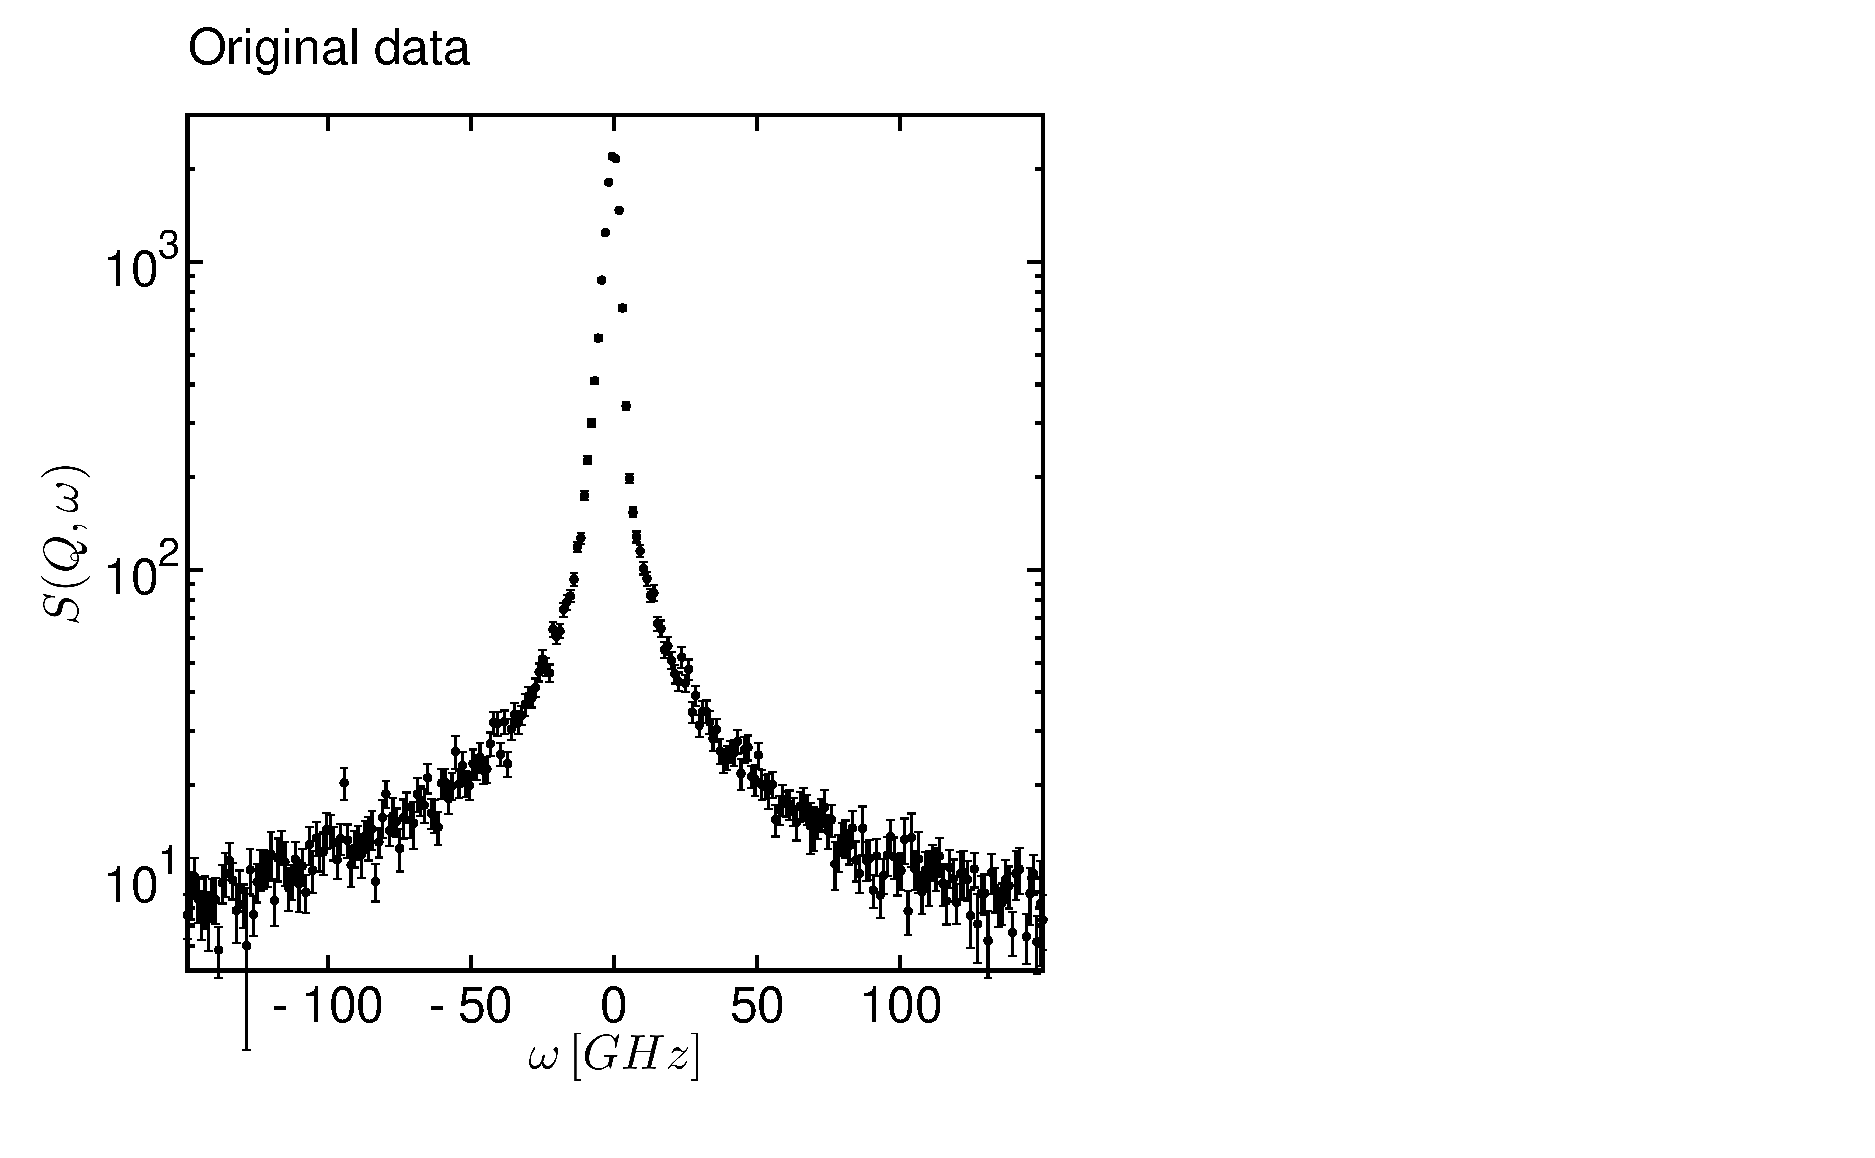
\includegraphics[bb= 50 50 600 600,width=0.5\textwidth]{dtrplot_Original_data-63.pdf}
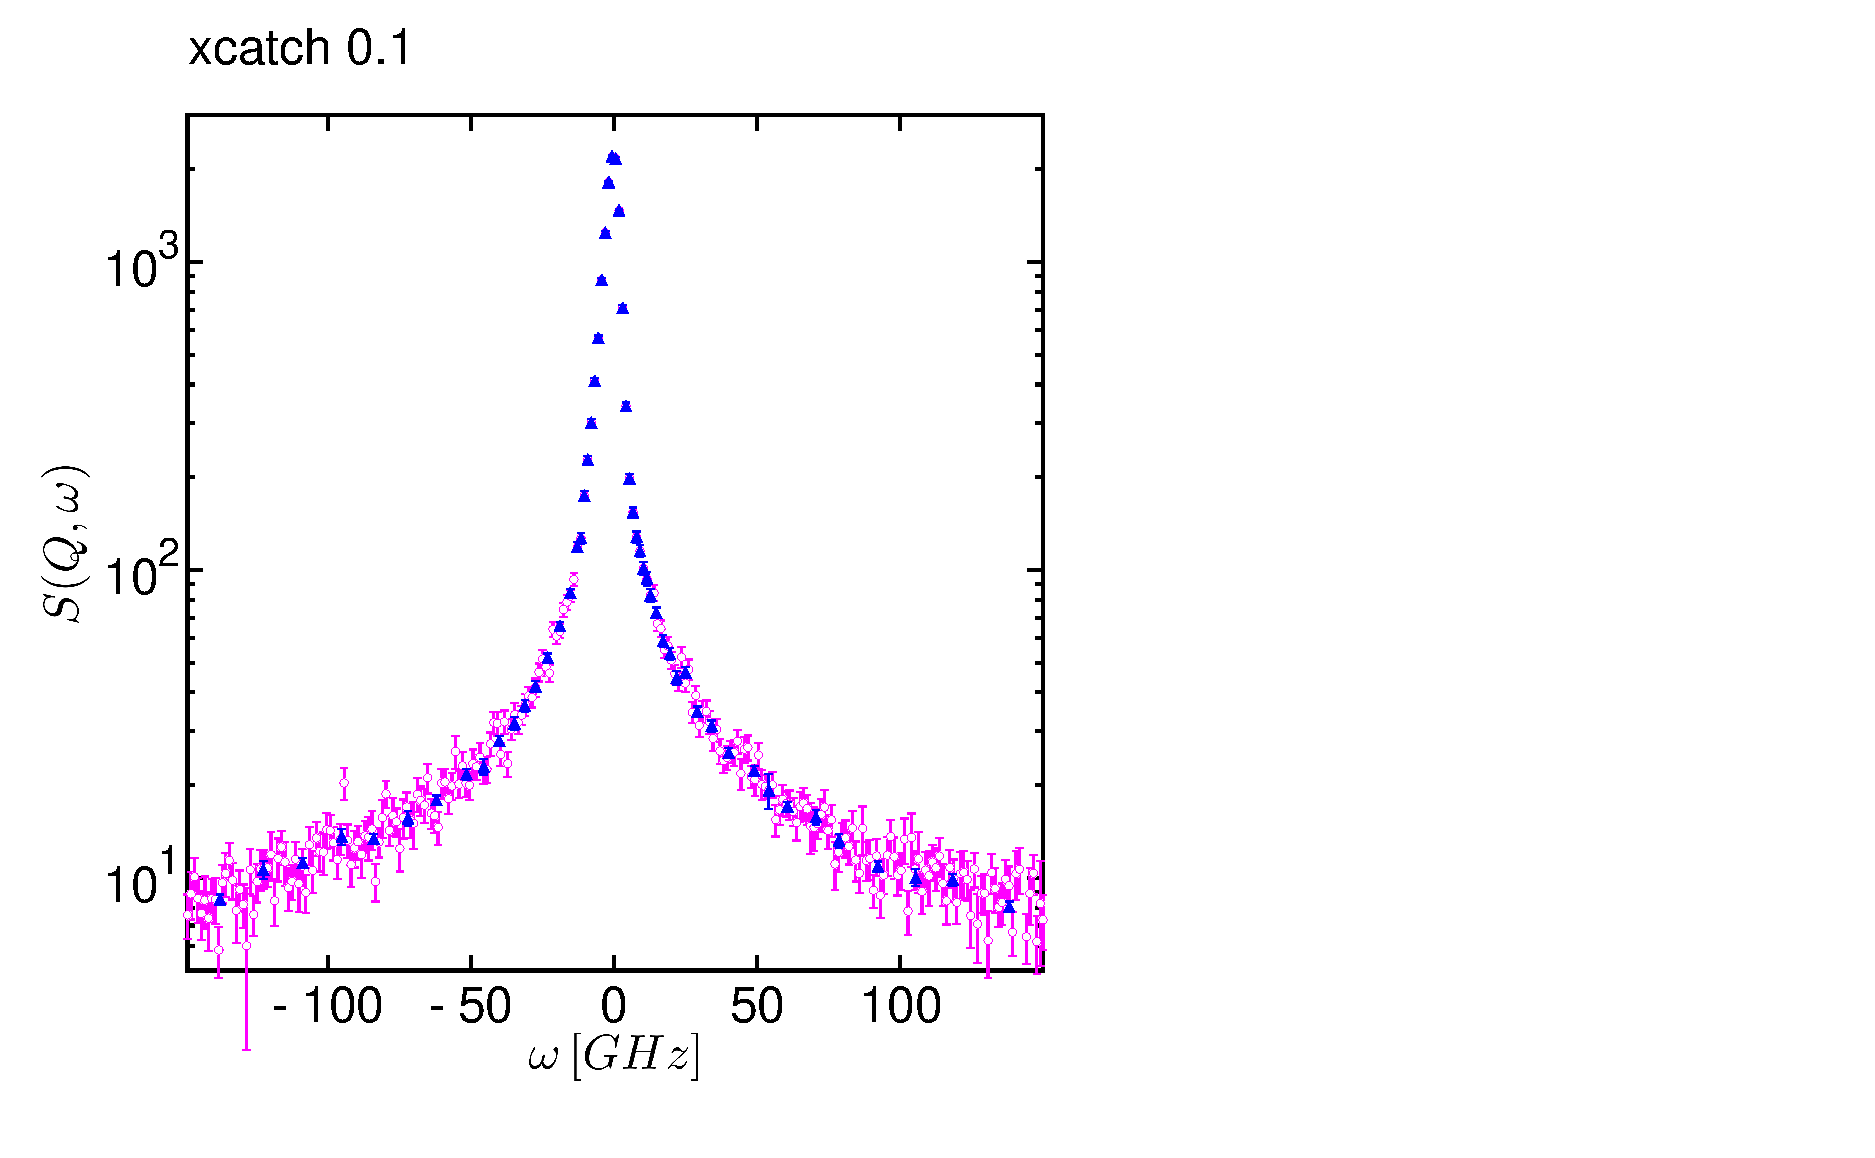
\includegraphics[bb= 50 50 600 600,width=0.5\textwidth]{dtrplot_xcatch_0p1-73.pdf}
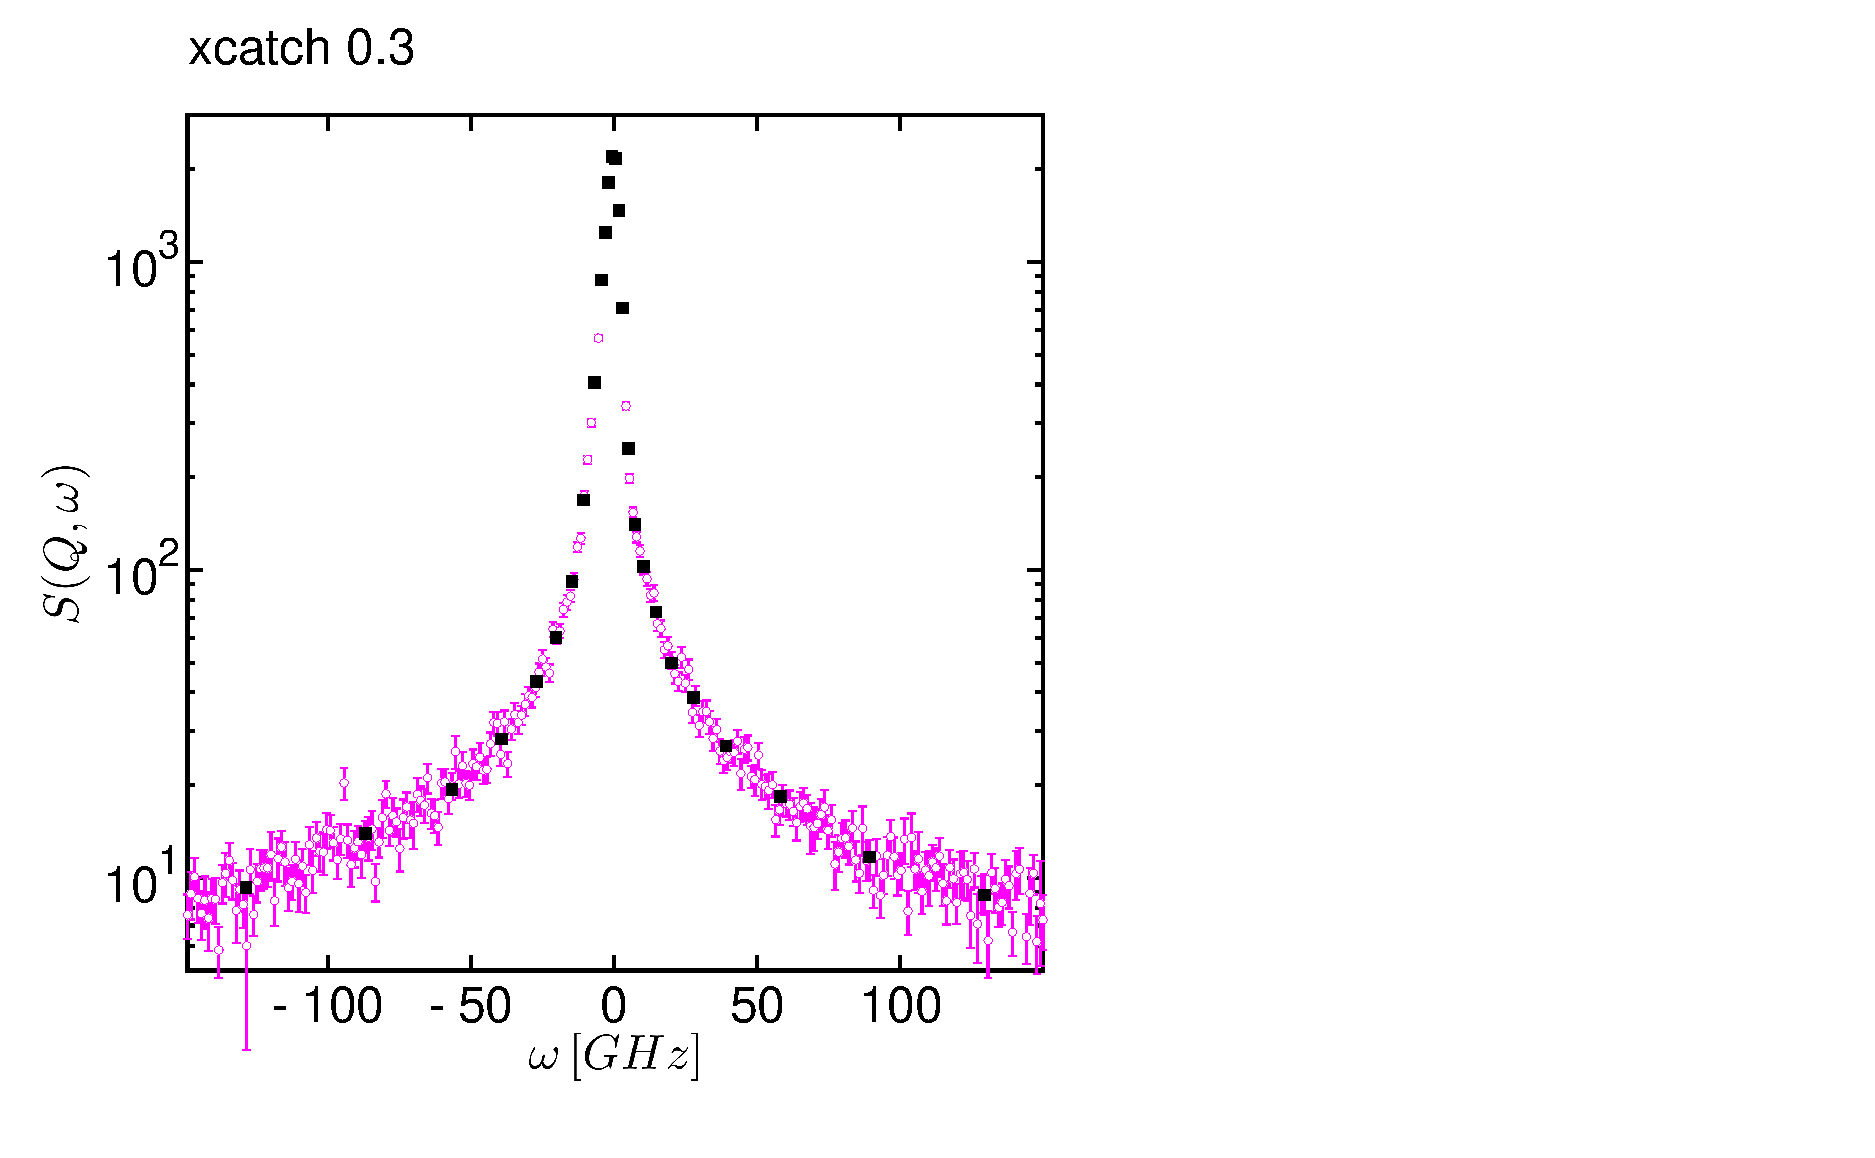
\includegraphics[bb= 50 50 600 600,width=0.5\textwidth]{dtrplot_xcatch_0p3-78.pdf}
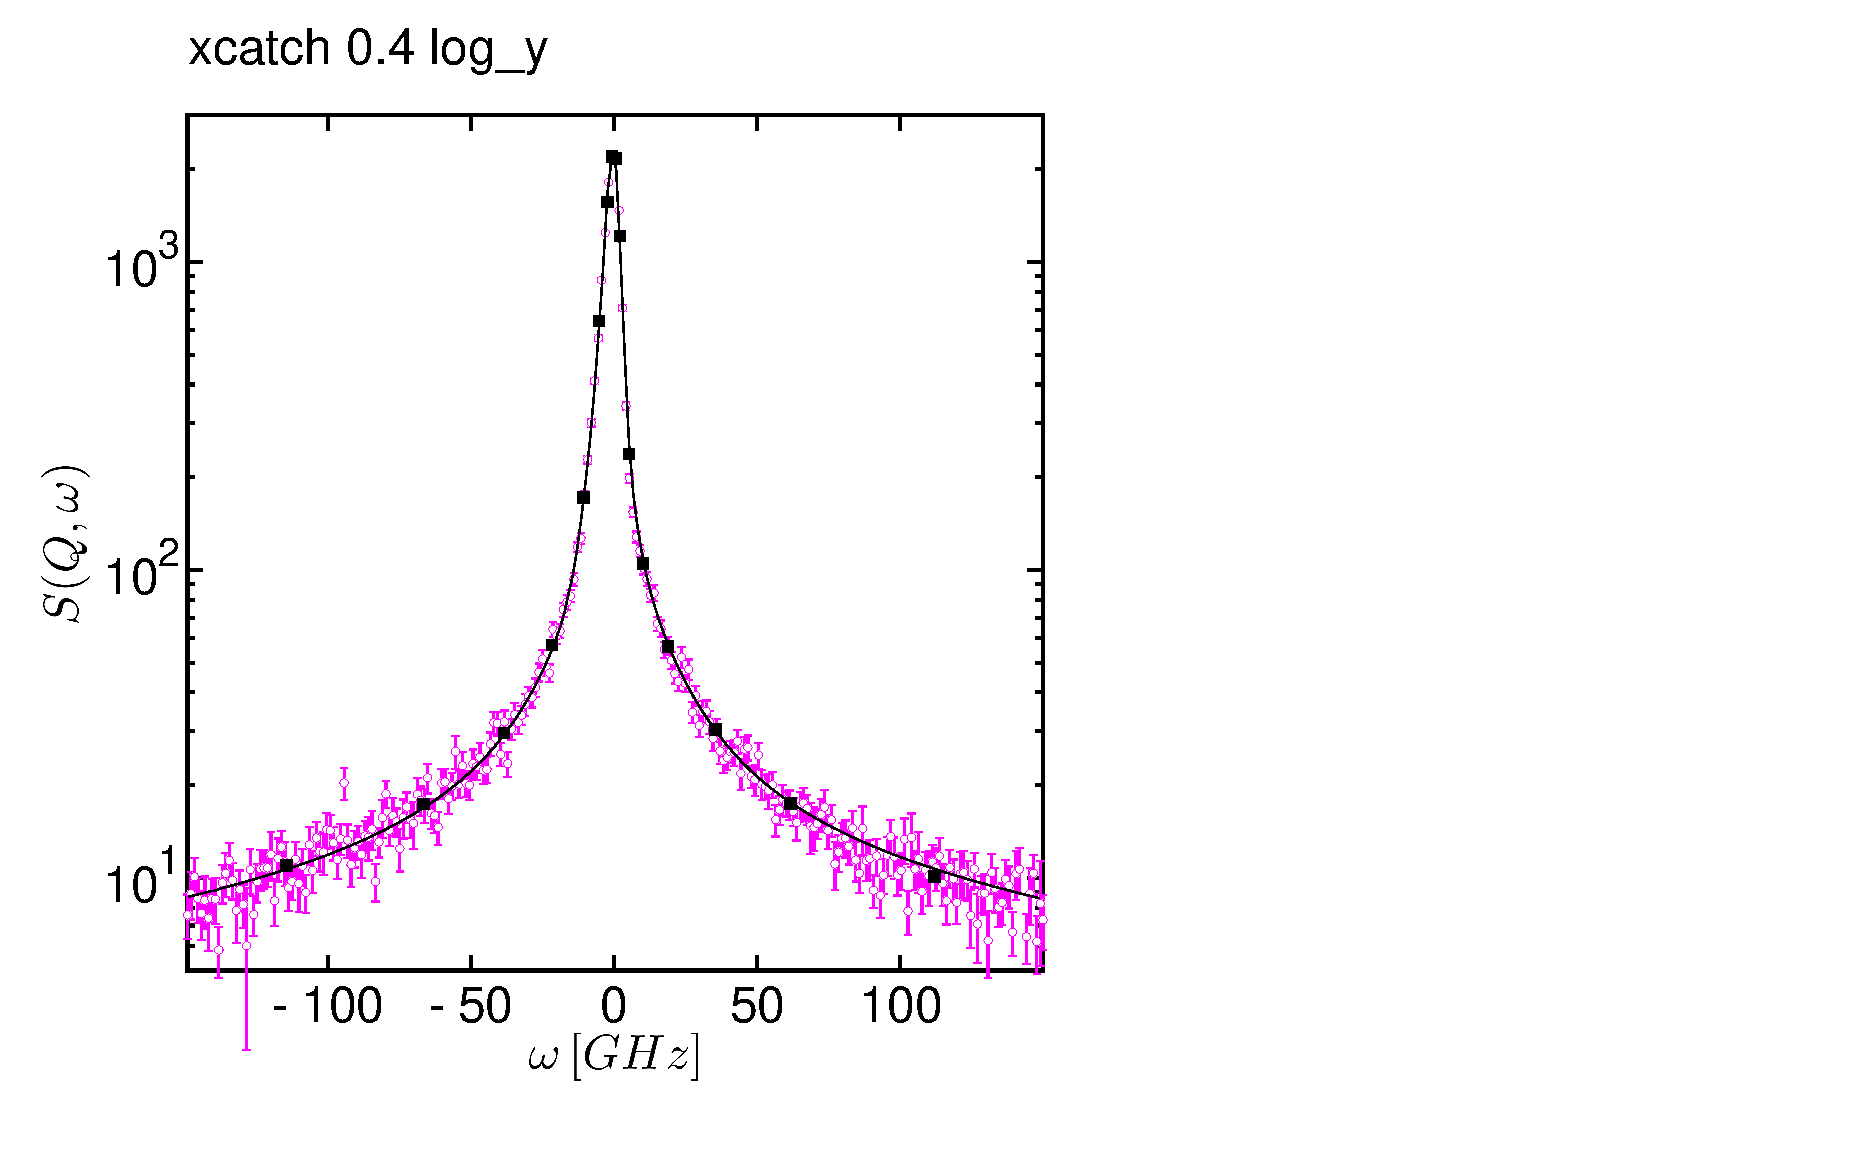
\includegraphics[bb= 50 50 600 600,width=0.5\textwidth]{dtrplot_xcatch_0p4-87.pdf}

\linespace
Illustrates the merging (and reduction in number) of points from a backscattering spectrum, always
starting from the original data and the applying {\bf average} with {\bf xcatch} = 0.1, 0.3, 0.4,
which yields the solid symbols in the plots. A fitted curve to the average results is shown for 
xcatch = 0.4. 

\linespace
{\bf Note 1:} The x-values of the result are different form the originals and generally not spaced
evenly (even if the originals were) but come out sorted in ascending order (even if the originals were not).

\linespace
{\bf Note 2:} Parameters of the result are weighted averages of the parameters of the contributing
records (if more than one were selected). {\bf Attention} in that case {\bf average} will only yield
sensible results if the selected records correspond to close by physical states and the range
of x-values covers approximately the same region.

\section{rebin \var{${nk}$} } 
\index{kz channel contraction}
\index{rebin x-channels}
Rebins the x-axis by adding the contents of ${nk}$ adjacent x-values (channels) and replacing it by
the {\bf average} values of ${x}$ and ${y}$, errors are treated accordingly.
The contraction is put to a new record. To perform it \emph{on place} use the otherwise equal
command {\bf kz} (with loss of the original content).

\begin{corollary}
\dtrprompt \cmdl{rebin}{${nk}$}  \return  \expl{averages over ${nk}$ x-channels.} 
\end{corollary}

\linespace
{\bf Note:} If data are non evenly spaced or have very different error bars on points with
close by x-values: use {\bf average} instead!

\section{rerange \var{${r_1}$} \var{${r_2}$}  \opt{y}} \index{rerange}
\index{restrict data range of a record}
\index{narrow data range of a record}
\index{exclude points from a record}
Removal of points outside the range \var{${r_1}$} $\cdots$ \var{${r_2}$} from the selected records.
If no option {\bf y} is given the range pertains the x-axis, with {\bf y} it pertains the y-axis.
The reduced data are stored with new record addresses. 

\begin{corollary}
\dtrprompt \cmdl{rerange}{\var{${r_1}$} \var{${r_2}$} } \return  
\end{corollary}

\linespace
{\bf Examples:}
\linespace
\begin{corollary}
\dtrprompt \cmdl{sel}{(j0)} \return \expl{select original record} \\
\dtrprompt \cmdl{rerange}{\var{${x1}$} \var{${x2}$} } \return  \expl{copy only x-range x1 x2 to new record } \\
\dtrprompt \cmdl{set}{(nbuf) j1} \return \expl{save the created address to j1} \\
\dtrprompt \cmdl{sel}{(j0)} \return \expl{select original record again} \\
\dtrprompt \cmdl{rerange}{\var{${x12}$} \var{${x22}$} } \return  \expl{copy another x-range x12 x22 to new record } \\
\dtrprompt \cmdl{sel}{add (j1) } \return  \expl{select also the previous range restricted record } \\
\dtrprompt \cmdl{average}{xcatch 0 } \return  \expl{recombine both ranges }
\end{corollary}
The above sequence is an example to prepare a more complex selection of x-values, e.g. for fitting.
The finally selected record contains the selected regions. Note: for fitting it would also suffice
to select all the partial ranges.

\begin{corollary}
\dtrprompt \cmdl{rerange}{0 (maxy+1) y } \return  \expl{keep only positive y-values } 
\end{corollary}

\section{alingny \opt{offset \var{o} yscale \var{ys} ostep \var{do}} ystep \var{dy} \desc{automatically adjust scales} }
\index{aligny}
\index{match record scales}
\index{offset}
\index{scale}
\index{combine records}

To determine offset and scale $(y+o) \times ys\rightarrow y$     
of second selected record in order to match the first selected record
use command {\bf aligny}!          
The scaled result is copied to a new record this and the "master" record are selected 
such that one may use {\bf average} to merge them.     
Applied scale and offset are put to the record parameters of the scaled second record.
                                              
\begin{corollary}
\dtrprompt \cmdl{alingny}{\opt{offset \var{o} yscale \var{ys} ostep \var{do} ystep \var{dy}} } 
\end{corollary}

The optional specification of \emph{offset}, \emph{yscale}, \emph{ostep} and \emph{ostep} enable
explicit specification of start values and step width for the Nelder-Mead simplex minimisation
procedure used here.

\linespace

{\bf Hint:} Excluding marginal points in the overlap region ({\bf rerange}) may
improve the accuracy of the result.
% --------------------------------------------------------------------------------------------------------------
\chapterimage{DatreatLogoFun.pdf} % Chapter heading image
\chapter{Transformation: applying functions to x and y}
\index{apply functions on x- and y-values}
\index{transform x- and y-values}
\index{f(x)->x}
\index{f(y)->y}

\section{fxy [op] x=\emph{(expressionX)}  y=\emph{(expression)}}
\vskip 1cm
% \begin{description}
% \item[op] Option: if present the results will replace the original data instead of creating new result records.
% \item[x=] Keyword needed to introduce (expressionX)
% \item[(expressionX)] is an expression that refers to the x-values as {\bf X} and y-values as {\bf Y} (and  
% y-errors as {\bf ERR}) also values of parameters, user- and system-varaibles can be used.
% The values are always extracted form the actaully proecessed record.
% It can contain binary operators {\bf  +, -, *, /, \Verb!^! } and functions: 
% {\bf {sqrt, exp, sin, cos, tan, atan, erf, J0, J1}}. The result replaces the x-values.
% \item[y=] Keyword needed to introduce (expressionX)
% \item[(expressionY)] is an expression as (expressionX) but the result replaces the y-values and corresponding
% y-errors.
% \end{description}
% \vskip 1cm

\begin{exercise}
\bf
Allows to transform the x-values and the y-values by functions. Errors in y are transformed accordingly.
The transformation is done for all selected records (is the sequence of selection), finally the resulting
transformed data records are selected.
\end{exercise}

\begin{corollary}
% \sysprompt \enter{cd \emph{Myworkingdirectory}} \return \\
\dtrprompt fxy [op] x=\emph{(expressionX)}  y=\emph{(expression)}   \return 
\end{corollary}


\linespace
{\bf Examples:}
\begin{corollary}
% \sysprompt \enter{cd \emph{Myworkingdirectory}} \return \\
\dtrprompt fxy x=X y=Y*X*X               \return \\
\dtrprompt fxy x=q\Verb!^!2*sqrt(wl4*X) y=Y \return 
\end{corollary}

where in the last line the \emph{parameter}, ${p^l}$, {\bf wl4} is used.

\newpage

\begin{tabular}{ | l | l | l | l | p{7cm} |}


\hline
  cmd item  &
  type      & 
  volatile  & 
  \# arg    & 
  descriptions \\ 
\hline\hline %-----------------------------------------------------------
  {\bf op}  &
  option    & 
  yes       & 
  0         & 
  If present the results will replace the original data instead of creating new result records. \\ 
\hline
  {\bf x=}  &
  keyword   & 
  no        & 
  (1)       & 
  Expects an expression for the transformation of x-values to follow. \\ 
 \hline
  {\bf (expressionX)}  &
  value string         & 
  no                   & 
  --                   & 
  is an expression that refers to the x-values as {\bf X} and y-values as {\bf Y} (and  
  y-errors as {\bf ERR}) also values of parameters, user- and system-variables can be used.
  The values are always extracted form the actually processed record.
  It can contain binary operators {\bf  +, -, *, /, \Verb!^! } and functions: 
  {\bf {sqrt, exp, sin, cos, tan, atan, erf, J0, J1}}. The result replaces the x-values. \\ 
  \hline
  {\bf y=}            &
  keyword             & 
  no                  & 
  (1)                 &  
  Expects an expression for the transformation of x-values to follow. May not occur prior to {\bf x=}.\\ 
 \hline
  {\bf (expressionY)}  &
  value string         & 
  no                   & 
  --                   & 
  is an expression as (expressionX) but the result replaces the y-values and corresponding
  y-errors.\\
\hline
\end{tabular}
\noindent

\vskip 1cm
\noindent
{\bf Actions:}
\vskip 0.5cm

\footnotesize
\noindent
\begin{tabular}{ | l | l | l | p{5cm} | l | l | l | }


\hline
  key         &
  source      & 
  dest        & 
  values      & 
  param.      & 
  numor       &
  names        \\ 
\hline\hline %-----------------------------------------------------------
  {\bf op}                                  &
  ${j_\mathrm{S} \in \cal{S}}$              & 
  ${j_\mathrm{R}=j_\mathrm{S} }$            & 
  --         & 
  --         & 
  --         & 
  --        \\ 
\hline
  {\bf x=}  &
  ${j_\mathrm{S} \in \cal{S}}$             &
  ${j_\mathrm{R} \rightarrow \cal{S}}$     & 
  ${x_j(i) = f_x(X,Y,ERR,{P^l},\{V^n\})}$;
   $X=x_j(i), Y=y_j(i), ERR=\delta y_j$;
   $P^l=p^l_j$ and $V^n$                   & 
  -- & 
  -- &
  xname ${\rightarrow f_x(\text{xname})} $\\ 
 \hline
  {\bf y=}  &
  ${j_\mathrm{S} \in \cal{S}}$             &
  ${j_\mathrm{R} \rightarrow \cal{S}}$     & 
  ${y_j(i) = f_y(X,Y,ERR,{P^l},\{V^n\})}$ \hfill and \hfill
  $\delta y_j(i) = |f_y(\dots, Y+\delta y/2)-f_y(\dots, Y+\delta y/2)|$; \hfill
  with
  $X=x_j(i), Y=y_j(i), ERR=\delta y_j$;
  $P^l=p^l_j$ and $V^n$       &            
  -- & 
  -- &
  xname ${\rightarrow f_y(\text{yname})} $\\ 
 \hline
\end{tabular}

\normalsize
%\emph{expression} is an expression that refers to the x-values as {\bf X} and y-values as {\bf Y} (and  
%y-errors as {\bf ERR}) also values of parameters, user- and system-varaibles can be used.
%The values are always extracted form the actaully proecessed record.
%It can contain binary operators {\bf  +, -, *, /, \Verb!^! } and functions: 
%{\bf {sqrt, exp, sin, cos, tan, atan, erf, J0, J1}}.
%
%The transformation is done for all selected records (is the sequence of selection), finally the resulting
%transformed data records are selected.
%
%The option {\bf op} tells the system to do the transformation "on place" instead of creating a new record
%for the transformed data.
\vskip 1cm
\noindent
{\bf Note:} It is discouraged to use the older commands: \emph{xformel, yformel, fun, funfun}, just use fxy instead!

% --------------------------------------------------------------------------------------------------------------
\chapterimage{DatreatLogoAdd.pdf} % Chapter heading image
\chapter{Arithmetic between data sets (records)}
\index{add two records}
\index{subtract two records}
\index{multiply y-values of two records}
\index{divide y-values of two records}

\section{arit f1 \var{(factor1)}  f2 \var{(factor2)}  [\vol{mult|div|vid}{}] [\vol{to}{numor}]}
\vskip 1cm

\begin{exercise}
\bf
Arithmetic combination of (exactly) 2 selected data-records. Default is ADDITION, options are
also MULTIPLICATIONS and DIVISION. Before combination the data are scaled by factor1 and factor2
respectively. The values of the seconds selection are interpolated to the x-values of the first
selection. The resulting record gets the x-values of the first selected record.
Errors are combined and transferred to the result. 
\end{exercise}

\begin{corollary}
% \sysprompt \enter{cd \emph{Myworkingdirectory}} \return \\
\dtrprompt arit f1 \var{factor1}  f2 \var{factor2} [\vol{mult}{|div|vid}] [\vol{to}{numor}]   \return 
\end{corollary}

\linespace
{\bf Examples:}
\begin{corollary}
% \sysprompt \enter{cd \emph{Myworkingdirectory}} \return \\
\dtrprompt arit                       \return  \\
\dtrprompt arit f1 1 f2 -1            \return  \\
\dtrprompt arit f1 1 f2  1  div       \return  \\
\dtrprompt arit f1 1 f2  1  to  7777  \return  
\end{corollary}

The first command (initial default still there) just adds selected records 1 and 2.

Next a subtraction selected record 1 - selected record 2 is executed.

Next a division record1/record2 is shown.

Finally the result is provided with a numor=7777.
\newpage
%\linespace

\begin{tabular}{ | l | l | l | l | p{7cm} |}
\hline
  cmd item  &
  type      & 
  volatile  & 
  \# arg    & 
  descriptions \\ 
\hline\hline %-----------------------------------------------------------
  {\bf f1}  &
  keyword   & 
  no        & 
  1         & 
  Set the factor for the (y)-data of the first selected record, initial default is 1. \\ 
\hline
  { \var{(factor1)} }  &
  value string         & 
  no (value)           & 
  0                    & 
  value or expression yielding the value of factor1.  \\ 
 \hline
  {\bf f2}  &
  keyword   & 
  no        & 
  1         & 
  Set the factor for the (y)-data of the first selected record, initial default is 1. \\ 
\hline
  { \var{(factor2)} }   &
  value string         & 
  no (value)           & 
  0                    & 
  value or expression yielding the value of factor1.  \\ 
\hline
  \vol{mult}{}          &
  option              & 
  yes                 & 
  0                   &  
  Instead of adding multiply the y-data of the selected records.\\ 
\hline
  \vol{div}{}           &
  option              & 
  yes                 & 
  0                   &  
  Instead of adding divide the y-data of the first records by those of the second record.\\ 
 \hline
  \vol{vid}{}           &
  option              & 
  yes                 & 
  0                   &  
  Instead of adding divide the y-data of the second records by those of the first record.\\ 
 \hline
  {\bf to}             &
  keyword              & 
  no                   & 
  1                    & 
  Set the result record numor to the following value.\\
 \hline
  \var{numor}          &
  value string         & 
  no                   & 
  --                   & 
  Numor to the record of the result values.\\
\hline
\end{tabular}


\linespace
\linespace

{\bf Actions:}
\linespace
\begin{align}
&  x_{j_1}(i)                       \rightarrow x_{j_d}(i)    \\
&  \left \{ f_1 \times y_{j_1}(i) \right \}
 \; +|*|/ \; 
\left \{ f_2 \times {\cal I}(\{y_{j_2}\},  x_{j_1}(i)) \right \} \rightarrow y_{j_d}(i)  
\end{align}
where ${{\cal I}(\cdots, x})$ denotes an interpolation.
\normalsize

{\bf Note:}
The determination of errors in the result record assumes that the errors pf the combined records are 
statistically independent!


\section{addsels}
\vskip 1cm
\index{add many records (addsels)}


\begin{exercise}
\bf
Addition of data from several (many) selected records. In this case the x-values must be the same
for all records. Example use: adding spectra from detectors of a TOF instrument. 
\end{exercise}

\begin{corollary}
% \sysprompt \enter{cd \emph{Myworkingdirectory}} \return \\
\dtrprompt addsels   \return 
\end{corollary}

Now the result record is selected.
Parameters of the summed records are averaged and the averages and their variances (indicated by prefix 'V') and the
number of contributing parameters (indicated by prefix 'N')  are updated/added to the parameter section
of the result record.



%           write(6,*)'=============================================================================='
%           write(6,*)'= recsum from <n1> to <n2>                                                    '
%           write(6,*)'=    creates record containing the sum of all records from a continuous       '
%           write(6,*)'=    address range <n1> .. <n2>      (similar addsels)                        '
%           write(6,*)'=============================================================================='
 
% --------------------------------------------------------------------------------------------------------------
\section{recsum from \var{rec1} to \var{rec2}}
\vskip 1cm
\index{add many consecutive records (recsum)}
\begin{exercise}
\bf
Addition of data from several (many) selected records -- as addsels -- but including the selection of a
continuous range of record numbers. In this case the x-values must be the same
for all records. Example use: adding spectra from detectors of a TOF instrument. 
\end{exercise}

\begin{corollary}
% \sysprompt \enter{cd \emph{Myworkingdirectory}} \return \\
\dtrprompt recsum from \var{rec1} to \var{rec2}   \return 
\end{corollary}

%           write(6,*)'=============================================================================='
%           write(6,*)'= recsum from <n1> to <n2>                                                    '
%           write(6,*)'=    creates record containing the sum of all records from a continuous       '
%           write(6,*)'=    address range <n1> .. <n2>      (similar addsels)                        '
%           write(6,*)'=============================================================================='
 


\chapterimage{DatreatLogoSpatcor.pdf} % Chapter heading image
\chapter{Special function scaling (spatcorr)}


\index{scaling, spatial correlation model, K1 q}
\index{spatcorr, scaling}

\section{spqscal}
\vskip 1cm

\begin{exercise}
\bf
Select any number of $S(q,t)/S(q)$ vs. $t$ spectra and combine these into a scaling plot using
parameters for a time dependent displacement function ${K_1(t)=\xi(t)}$ [{\it PRE  104, 024503 (2021)}]  
that immediately prior to \textbf{ spqscal} have been fitted. 
\begin{equation}
\xi^2 = 
{\it r^2}\, \left[  \left\{  \left( {\frac {t}{\tau}} \right) ^{-\nu_1}
 \right\} ^{a}+ \left\{  \left( {\frac {t}{\tau}} \right) ^{-\nu_2}
 \right\} ^{a} \right] ^{-{1/a}}
\end{equation}
with exp1 = ${\nu_1}$ and exp2 = ${\nu_2}$.
\end{exercise}

\linespace
{\bf Examples:}
\begin{corollary}
% \sysprompt \enter{cd \emph{Myworkingdirectory}} \return \\
\dtrprompt in in15runs                       \return  \\
\dtrprompt sel 1 -20                         \return  \\
\dtrprompt ac spatcor2                       \return  \\
\dtrprompt cth                               \return  \\
\dtrprompt   ... enter start parameters      \return  \\
\dtrprompt fit                               \return  \\
\dtrprompt spqscal                           \return  \\
\dtrprompt fxy x=X*X y=Y  ! scale vs (K1*Q)**2                  \return  
\end{corollary}




\part{Fitting}

% --------------------------------------------------------------------------------------------------------------
\chapterimage{DatreatLogoFit.pdf} % Chapter heading image
\chapter{Model fitting}
\index{fitting}
\index{model fitting}

One of the central purposes of \emph{datreat} is model fitting, either to a combination of 
available (predefined) model function or to custom made new model functions as described 
in chapter \ref{ch:newmod}.
It is possible to fit several data-records simultaneously, the applied function may then be
discriminated by the metadata parameters ${p_j^m}$ associated with each record $j$. 

\section{th \opt{name}   \desc{display information on available theories}}
The first step needed is the specification of the model to be fitted. Here we describe how
this is achieved by using the actual predefined \emph{theories}.
\linespace
To get an overview of the available \emph{theories} (alphabetically ordered list of names):

\begin{corollary}
% \sysprompt \enter{cd \emph{Myworkingdirectory}} \return \\
\dtrprompt \cmdl{th}{}   \return
\color{blue}
\footnotesize
\begin{verbatim}
> th
 ***** available theories available *****
 ---------------------------------------------------------------------------------
  anisodi   beaucage  benoitmf  bkgr      d2sphere  ddiavo    debstar   debye2  
  degenne2  degennea  degennes  diffusio  dirosp    dolgushe  echo      echotri2
  eval      gauss     gauss2    gaussft   hetdif    hetdifq   hyperbra  kohl_q  
  kohlfast  likhtman  ln_bss1   locrep    locrep2   locrep3   lrep2nr   moderato
  ndebye    ndendpy   ndendri   nmrdiff   nmrdiff2  nmrdiff3  nnvilgis  nrouconf
  nrous_22  nrous_s2  nrous_s4  nrousefn  nrousefy  nrousep   nrouserr  nvilgis 
  nzimm_pn  nzimm_s   nzimmaz   peryev    q**n      repmode2  riggch    ring2   
  ring2a    roufbead  rouse     rpalin    rpastar2  rpastar3  sansfac   shell3_f
  sinhafra  sofq      srouse    star      strexpo   strexpsq  strexsqq  thickco2
  thickco4  zgbic2    zglam1    zimm    
 ----------------------------------------------------------------------------------

  .... for more details on one of these: --> th <theoryname> ! 
\end{verbatim}
\normalsize
\color{black} 
\end{corollary}

\linespace
In order to get more details on a specific theory use:
\begin{corollary}
% \sysprompt \enter{cd \emph{Myworkingdirectory}} \return \\
\dtrprompt \cmdl{th}{theoryname}   \return
\end{corollary}
{\bf Example:}
\begin{corollary}
% \sysprompt \enter{cd \emph{Myworkingdirectory}} \return \\
\dtrprompt \cmdl{th}{nrousep}   \return
\color{blue}
\footnotesize
\begin{verbatim}
 > th nrousep
-----------------------------------------------------------------------------------
theory id-name: nrousep 
-----------------------------------------------------------------------------------
 Rouse by discrete summation with mode restriction
                 ACCELERATED (OMP+IMPOVED ALG.) VERSION!
-----------------------------------------------------------------------------------
Parameters( 8): 
  1: amplitu  > prefactor
  2: wl4      > rouse rate
  3: n_segmen > effective N for summation
  4: re       > end-to-end radius of Gaussian coil
  5: temp     > temperature if not in parameters
  6: com_diff > center of mass diffusion (if 0, use Rouse default)
  7: pmin     > minimum mode to be included
  8: pmax     > maximum mode to be included
++++++++++++++++++++++++++++++++++++++++++++++++++++++++++++++++++++++++++++++++++
INPUT: Parameters that are extracted from the actual considered data records:
..there may be default assumptions, but better make sure that these parameters are set properly!
  1: q        > momentum transfer
  2: temp     > temperature
===================================================================================
OUTPUT: Parameters that are computed and added to the records parameters as information:
  1: diff     > diffusion in cm**2/s
  2: l        > effective segment length
  3: w        > rouse rate: W
  4: wl4      > inferred value of Wl4
...................................................................................
cite:  Rouse, Doi_Edwards !
-----------------------------------------------------------------------------------
\end{verbatim}
\normalsize
\color{black} 
\end{corollary}

\section{activate \var{name} \opt{multiply|insert} \opt{range ...}   \desc{Add a theory to the active list}}
\index{activate theories}
\index{chain theories (insert)}
\index{insert theories (chain)}
\index{combine theories}
\index{model definition}


\begin{exercise}
Add a new (instance) of an available theory to the model definition. 
Normally the resulting value from the new activated theory is added to the result of the 
result of the preceding theories.
\end{exercise}

\begin{corollary}
% \sysprompt \enter{cd \emph{Myworkingdirectory}} \return \\
\dtrprompt \cmdl{ac}{theoryname}   \return
\end{corollary}
If the option \opt{multiply} is specified the resulting value from the new activated theory is 
{\bf multiplied} to the result of the result of the preceding theories instead.
\begin{corollary}
% \sysprompt \enter{cd \emph{Myworkingdirectory}} \return \\
\dtrprompt \cmdl{ac}{theoryname multiply}    \return
\end{corollary}
If the option \opt{insert} is specified the resulting value from the {\bf previous} activated theories is 
{\bf inserted} as independent variable into this theory.
\begin{corollary}
% \sysprompt \enter{cd \emph{Myworkingdirectory}} \return \\
\dtrprompt \cmdl{ac}{theoryname insert}    \return
\end{corollary}
\linespace
The current state of the modeled definition can be displayed using {\bf a}ctive{\bf l}ist:
\begin{corollary}
% \sysprompt \enter{cd \emph{Myworkingdirectory}} \return \\
\dtrprompt \cmdl{al}{}    \return
\end{corollary}
\linespace

\begin{exercise}
Any present theory model definition can be cleared by deactivate theory:
\end{exercise}

\begin{corollary}
% \sysprompt \enter{cd \emph{Myworkingdirectory}} \return \\
\dtrprompt \cmdl{dac}{}    \return
\end{corollary}
\linespace
 
{\bf Example:}
\begin{corollary}
% \sysprompt \enter{cd \emph{Myworkingdirectory}} \return \\
\dtrprompt \cmdl{dac}{}   \return  \\
\dtrprompt \cmdl{ac}{strexpo}   \return \\
\dtrprompt \cmdl{ac}{strexpo multiply}   \return \\
\dtrprompt \cmdl{ac}{bgr             }   \return \\
\color{blue}
\footnotesize
\begin{verbatim}
...
...
 > al
  ***** activated theories *****
 current parametersetting:
 theory   strexpo                                                                         
      amplitu     0.000000       0.00       0.0000    
      tau         0.000000       0.00       0.0000    
      beta        0.000000       0.00       0.0000    
      qexp        0.000000       0.00       0.0000    
 theory   strexpo    multiply                                                             
      amplitu     0.000000       0.00       0.0000    
      tau         0.000000       0.00       0.0000    
      beta        0.000000       0.00       0.0000    
      qexp        0.000000       0.00       0.0000    
 theory   bkgr                                                                            
      level       0.000000       0.00       0.0000    
      slope       0.000000       0.00       0.0000    
 end\end{verbatim}
\normalsize
\color{black} 
\end{corollary}
Here the defined model function (with no physical sense) would be:
\begin{equation}
f_\mathrm{model} = a_1 \exp(-(x/\tau_1)^{\beta_1}) \times a_2 \exp(-(x/\tau_2)^{\beta_2}) 
+ ( b_\mathrm{level} + x  b_\mathrm{slope} ) 
\end{equation}
as you may note here all parameters still have value 0. 
So in the next step these have to be given (start) values and selection which
are to be fitted.

\section{cth \desc{Change/set (edit) theory model parameters}}
\index{change fitting parameters (cth)}
\index{edit fitting parameters (cth)}
\index{enter fitting parameters (cth)}


\begin{exercise}
The command (makro call) {\bf c}hange{\bf th}eory can be used to set up the theory model
parameters and to control which parameters shall be fitted.
It opens an editor which allows editing:
\end{exercise}

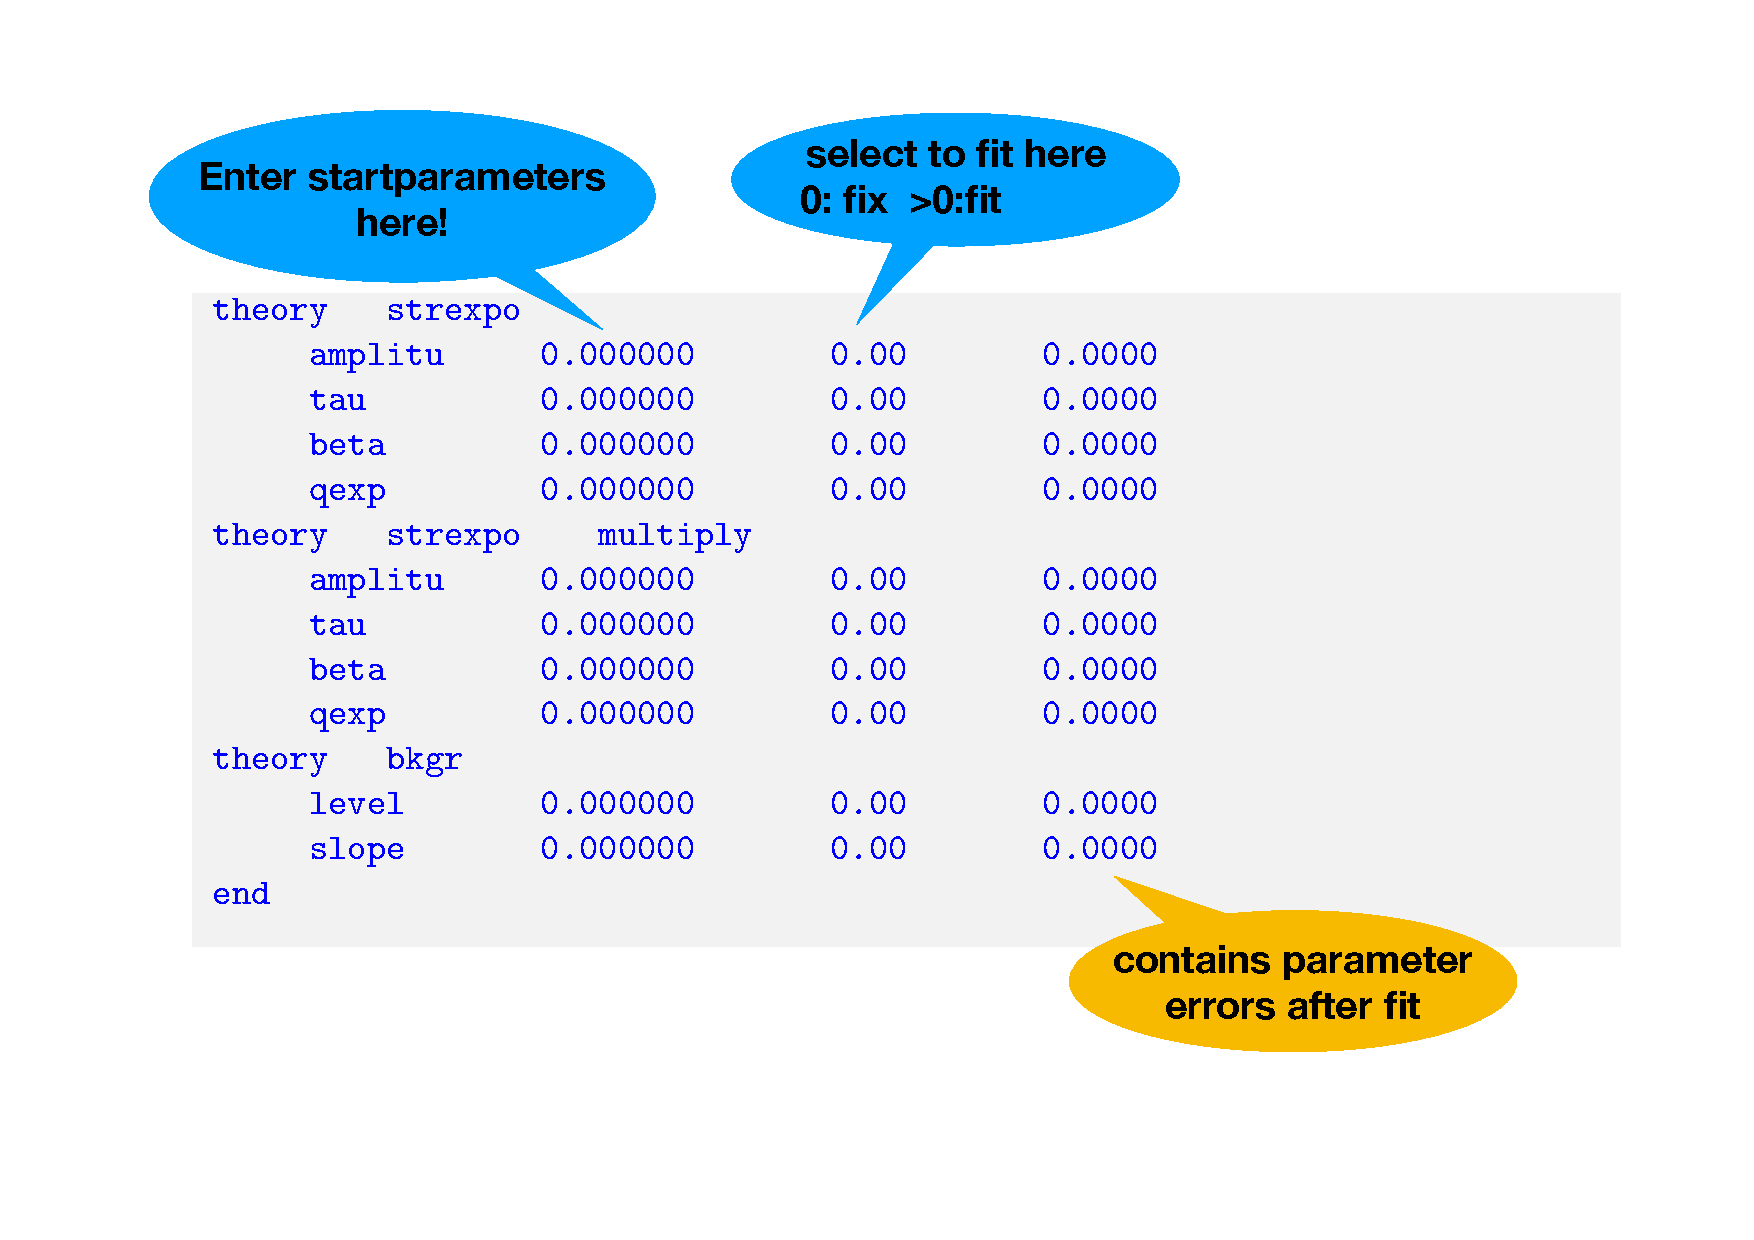
\includegraphics[width=0.9\textwidth]{thparexplan1.pdf}

The first numerical column represents the (start) parameters of the theory. The second column
selects parameters for fitting. A zero value means that the parameter shall be held fixed, if it shall
be fitted is must be set to a value in the order of magnitude of the expected parameter value.

The third column may contain parameter errors determined by a (previous) fit step, here they can
be ignored.
\linespace

{\bf Note 1:} Numerical input here may also be an {\it expression}, it will be evaluated upon rereading the
model definition and the replaced by the corresponding value.
\linespace

{\bf Note 2:} Theories may be removed or added at this level by deleting or inserting the text blocks
starting with \emph{theory}.
\linespace

{\bf Note 3:} {\bf cth} is a makro the opens an editor with file \emph{lastth} thus allowing editing. After
leaving the editor then it executes the command {\bf acl} to read the contents of lastth.
The preferred editor can be set in datreat/makros/cth. \tbd{make editor selection global!}
\linespace

{\bf Note 4:} Check that the new theory is correctly displayed in the \emph{datreat} window. If not 
directly reissue {\it cth} and correct typos or other errors.
\linespace

{\bf Note 5:} For more advanced fitting options like parameter coupling, record selective theories,
restriction of fitted points etc. see chapter \ref{cha:advfit}!

\section{thc \desc{compute the theory model}}
\label{sec:thc}
%

\begin{exercise}
{\bf th}eory{\bf c}ompute computes the theory at the x-values of the selected records or on
a specified x-range.
\end{exercise}

\begin{corollary}
% \sysprompt \enter{cd \emph{Myworkingdirectory}} \return \\
\dtrprompt \cmdl{thc}{}   \return  \\
\dtrprompt \cmdl{thc}{ \color{magenta} n \var{np}  x1 \var{x1}  x2 \var{x2} \color{black}}   \return
\end{corollary}
the second line is the form to specify th x-range to be computed, \var{np} denotes the number
of points per curve (record) to be computed and \var{x1} $\cdots$ \var{x2} is the x-range to be covered.
If \var{n} $< 0$ then the x-axis division is logarithmic (use this if \emph{log\_x}-plots are intended.
\linespace

{\bf Note 1:} The computed curves are stored with new record addresses that are internally associated with
the selected data-records. Plotting automatically displays the computed curves as lines with the same
color as the pertaining data.  
\linespace

{\bf Note 2:} The numerical-id \emph{numor} of the computed curve is the negative of the parent data record numor.
\linespace

{\bf Note 3:} {\bf The automatic association of data and fit is removed as soon as a new \cmdl{sel}{} has
been issued.}

\section{fit \desc{Fitting the model parameters to data}}
%

\begin{exercise}
Fits the theory model (setup see above) to the selected records at the x-values over
a specified x-range.
\end{exercise}

Fits the theory model (setup see above) to the selected records at the x-values over
a specified x-range.
\begin{corollary}
% \sysprompt \enter{cd \emph{Myworkingdirectory}} \return \\
\dtrprompt \cmdl{fit}{}   \return  \\
\dtrprompt \cmdl{fit}{maxfn \var{m}}   \return  \\
\dtrprompt \cmdl{fit}{ x1 \var{x1}  x2 \var{x2} }   \return
\end{corollary}
the first line initiates fitting with the (current | default) range settings. The second form
allows to modify the maximum (approximately) allowed number of model evaluations \var{m}.
The third line shows how to restrict the x-range for fitting ({\bf permanent} until changed.

The model with the resulting parameters is automatically computed at the end of the fit and all remarks 
and notes to {\bf thc} (section: \ref{sec:thc}) apply.
\linespace

Finally use \cmdl{plot}{} to view the result.


{\bf Note:} More on fitting in the next chapter and in chapter \ref{cha:workex}.
% -------------------------------------------------------------------------------------------------------------
\chapterimage{DatreatLogoFit.pdf} % Chapter heading image
\chapter{Advanced fitting topics}
\label{cha:advfit}

\section{Coupling of parameters and record selective theories}
\index{coupling (fit parameters)}
\index{fit (coupling parameters)}
\label{sec:coupling}
It may be desired that some fit-parameters in a \emph{theory model} have a {\bf fixed} relation,
i.e. are coupled. Further it may be desired to assign specific instances of a theory to
a subset of all data-records that are fitted simultaneously. The records are to be discriminated
by a record related parameter (in the following example this parameter has the name {\bf \_xwidth}).
\linespace
First (max. 4 characters wide) {\bf labels} are assigned to each of the lead parameters 
(those that are fitted). The dependent parameters then are {\bf coupled} by a sequence of
{\bf label} {\bf coefficient}. During fit a dependent parameter ${p_d}$ then gets the value:
\begin{equation}
\label{eq:X}
p_d = p_d^0 + \sum_{\{i\}}{c_{i,d} \, (p_i-p_i^0)}
\end{equation}  
where ${p^0}$ means the starting value of a theory parameter, ${p_i}$ any (labelled) lead parameter,
${c_{i,d}}$ the coupling coefficient and ${\{i\}}$ the set of parameters (indices) that are coupled to
${p_d}$.
\linespace
The easiest way to setup parameter coupling is to \emph{activate} the required theories
and do the further editing using {\bf cth}  (command line/makros methods: see below).
In the following an example is shown to illustrate the structure of the required input.
\small
\begin{verbatim}
 theory   kohlfast              range _xwidth  min   3.00000     max   10000.0            
      intensit    1.000000       1.00       0.0000    
      n_chain    0.7000000       0.00       0.0000    
      n_ch3      0.3000000       0.00       0.0000    
 tkww tau_kww     1.256255      0.100      0.54915E-01
 bkww beta_kww   0.5300000       0.00       0.0000    
 lnt  lntau_mg   -3.495569      0.100      0.16992    
 si   sigma_mg   0.1000000       0.00       0.0000    
      beta_mg     1.000000       0.00       0.0000    
      rhh         1.780000       0.00       0.0000    
 u    u_square    0.000000       0.00       0.0000    
      omega0    -0.3262012       0.00       0.0000    
      epsilon    0.1000000E-06   0.00       0.0000    
      xwidth      0.000000       0.00       0.0000    
 ei   eisf2      0.6478480      0.100      0.58930E-02
 tf   tau_fast   0.1655679E-02  0.100E-04  0.79312E-04
 bf   beta_fas   0.6480139       0.00       0.0000    
 theory   kohlfast              range _xwidth  min   0.00000     max   3.00000            
      intensit    1.000000       1.00       0.0000    
      n_chain    0.7000000       0.00       0.0000    
      n_ch3      0.3000000       0.00       0.0000    
      tau_kww     1.256255       0.00       0.0000       tkww    1.000000    
      beta_kww   0.5300000       0.00       0.0000       bkww    1.000000    
      lntau_mg   -3.495569       0.00       0.0000       lnt     1.000000    
      sigma_mg   0.1000000       0.00       0.0000       si      1.000000    
      beta_mg     1.000000       0.00       0.0000    
      rhh         1.780000       0.00       0.0000    
      u_square    0.000000       0.00       0.0000       u       1.000000    
      omega0     0.2452426       0.00       0.0000    
      epsilon    0.1000000E-06   0.00       0.0000    
      xwidth      0.000000       0.00       0.0000    
      eisf2      0.6478480       0.00       0.0000       ei      1.000000    
      tau_fast   0.1655679E-02   0.00       0.0000       tf      1.000000    
      beta_fas   0.6480139       0.00       0.0000       bf      1.000000    
 end
\end{verbatim}
\normalsize

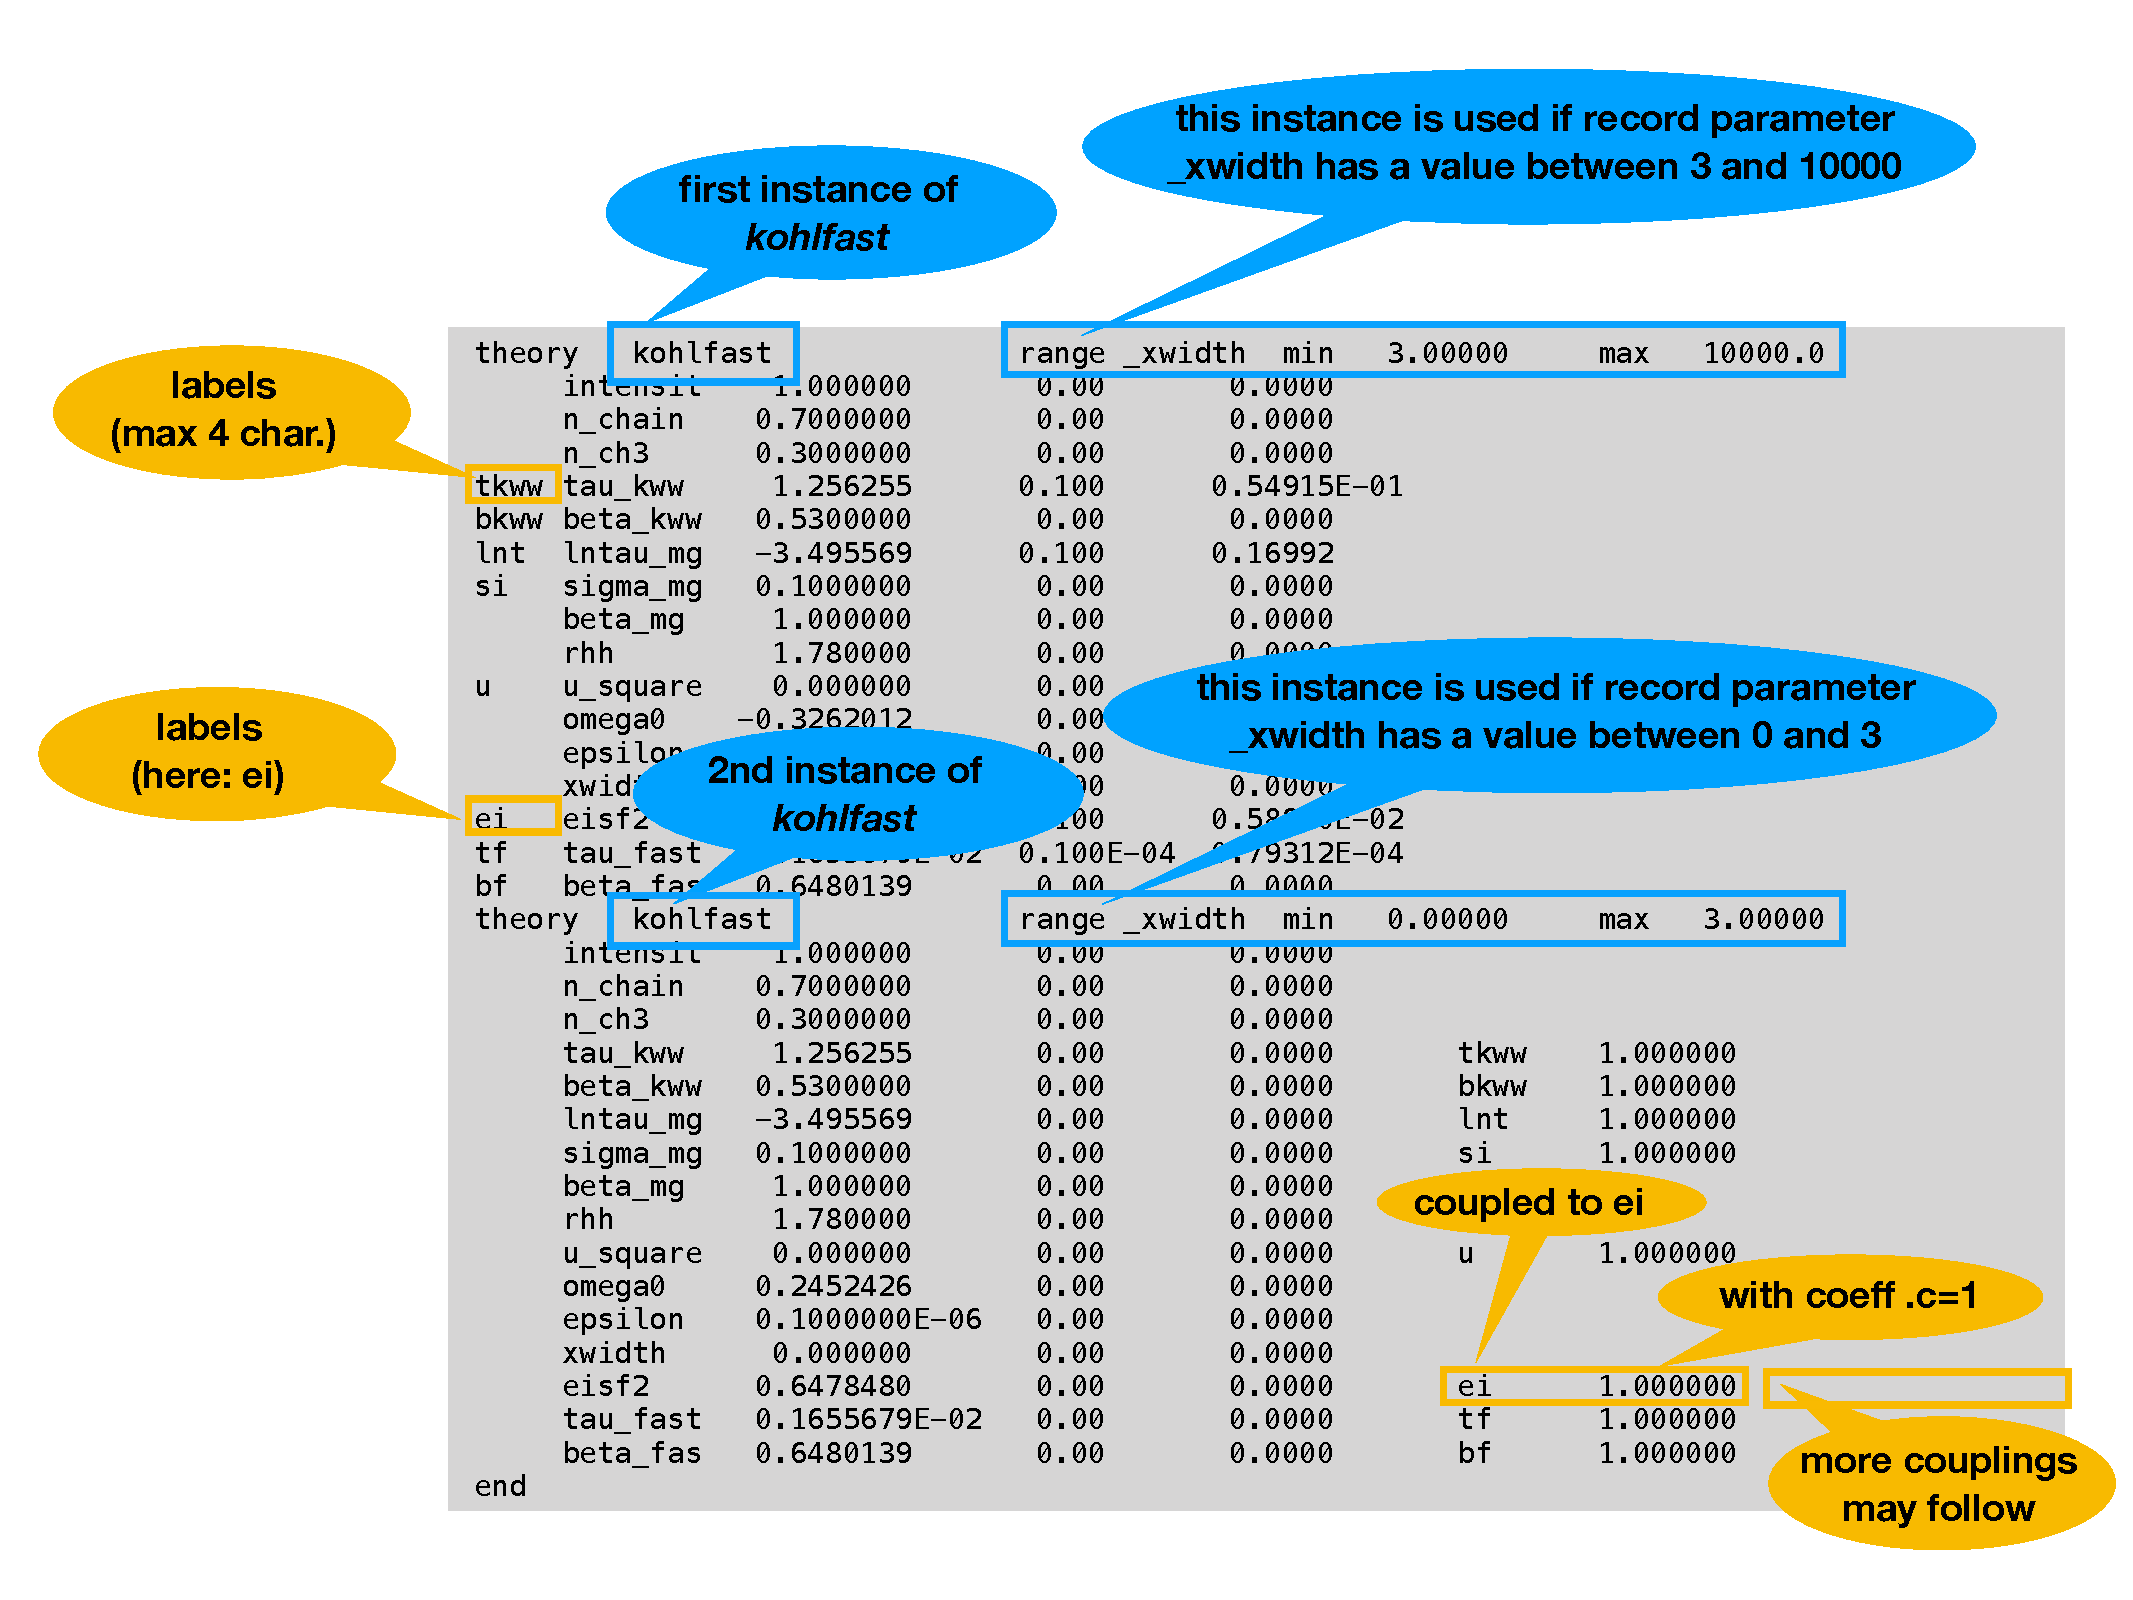
\includegraphics[width=\textwidth]{couplingdiagramm.pdf}

The example illustrates the case that spectra form two instruments (backscattering and tof) 
with possibly different intensity scaling, different resolution (given by record related parameters)
are to be fitted simultaneously. The \emph{range} selection discriminates the instruments by the
channel width record parameter \emph{\_xwidth} and in the theory the sample related physical 
parameters are kept equal in both instances of the theory \emph{kohlfast} by coupling. To achieve that 
these parameters are provided with \emph{labels} in the first instance and these labels are
used in the second instance to specify the couplings. In this case the parameters shall always
have the same value, therefor there is one {\bf coupling coefficient = 1} and the corresponding
\emph{starting values must be the same}!

\linespace

{\bf Note 1:} in cases like this (coupling = 1) \emph{datreat} will issue a \emph{warning} if the
starting values differ. (Use coupling = 0.99999 to avoid the warning if the unequal starting
point setting is (exceptionally) intended! 

\linespace

{\bf Note 2:} in cases where the sum of two parameters shall be kept (i.e. total amplitude) use
(coupling(s) = -1)!

\section{theory range \var{pnam} min \var{p1} max \var{p2} \desc{selective application to records}}
\index{fit (record selective theory)}
\index{range (theory)}
If a record parameter associated range shall be associated to a theory instance this
has to be specified when the theory is activated.

\begin{corollary}
% \sysprompt \enter{cd \emph{Myworkingdirectory}} \return \\
\dtrprompt \cmdl{ac}{thnam \opt{multiply} range rparname min \var{value} max \var{value} }   \return  
\end{corollary}

Activates a new instance of theory \emph{thnam} (optionally as \emph{multiply} and active if the
record parameter \emph{rparname} has a value between the specified min-max values.

\section{chgthpar \var{var} \var{p} scale \var{fs}  \desc{command line fit parameter setting}}
\index{chgthpar}
\index{change theory parameter, command}
\index{set theory parameter, command}

\begin{exercise}
{\bf chgthpar} allows the specification of single theory parameters via command (particular
useful in makros).
\end{exercise}

\begin{corollary}
% \sysprompt \enter{cd \emph{Myworkingdirectory}} \return \\
\dtrprompt \cmdl{chgthpar}{thnam \var{instance} parname par \var{value} scale \var{value} }   \return  
\end{corollary}

\linespace

{\bf Example:}
\begin{corollary}
\dtrprompt dac \return \expl{clear theory definition}  \\
\dtrprompt ac bkgr  \return \expl{activate theory \it bkgr}  \\
\dtrprompt ac ndebye  \return \expl{activate theory ndebye}  \\ 
\dtrprompt chgthpar bkgr  1 level     par 0.1      scale 0.01  \return \expl{set parameter and fit scale}  \\ 
\dtrprompt chgthpar bkgr  1 slope     par 0.0      scale 0 \return \\
\dtrprompt chgthpar ndebye 1 ampli    par    0.01        scale  0.01     \return \\
\dtrprompt chgthpar ndebye 1 n        par   333          scale  0.00     ! do not fit !   \return \\
\dtrprompt chgthpar ndebye 1 l        par    10          scale  0.100      \return \\
\dtrprompt chgthpar ndebye 1 nu       par    0.4         scale  0.100      \return \\
\dtrprompt chgthpar ndebye 1 chi      par    1e-3        scale  1e-3      \return \\
\dtrprompt chgthpar ndebye 1 withsq   par    1           scale  0.0       \return \\
\dtrprompt al \return \\
\out{~~*****~activated~theories~*****~~~~~~~~~~~~~~~~~~~~~}~\\
\out{~current~parametersetting:~~~~~~~~~~~~~~~~~~~~~~~~~~~}~\\
\out{~theory~~~bkgr~~~~~~~~~~~~~~~~~~~~~~~~~~~~~~~~~~~~~~~}~\\
\out{~~~~~~level~~~~~~0.1000000~~~~~~0.100E-01~~~0.0000~~~}~\\
\out{~~~~~~slope~~~~~~~0.000000~~~~~~~0.00~~~~~~~0.0000~~~}~\\
\out{~theory~~~ndebye~~~~~~~~~~~~~~~~~~~~~~~~~~~~~~~~~~~~~}~\\
\out{~~~~~~ampli~~~~~~0.1000000E-01~~0.100E-01~~~0.0000~~~}~\\
\out{~~~~~~n~~~~~~~~~~~333.0000~~~~~~~0.00~~~~~~~0.0000~~~}~\\
\out{~~~~~~l~~~~~~~~~~~10.00000~~~~~~0.100~~~~~~~0.0000~~~}~\\
\out{~~~~~~nu~~~~~~~~~0.4000000~~~~~~0.100~~~~~~~0.0000~~~}~\\
\out{~~~~~~chi~~~~~~~~0.1000000E-02~~0.100E-02~~~0.0000~~~}~\\
\out{~~~~~~withsq~~~~~~1.000000~~~~~~~0.00~~~~~~~0.0000~~~}~\\
\out{~end~~~~~~~~~~~~~~~~~~~~~~~~~~~~~~~~~~~~~~~~~~~~~~~~~}~\\
\out{~end~of~data~~~~~~~~~~~~~~~~~~~~~~~~~~~~~~~~~~~~~~~~~}~\\
\end{corollary}

\linespace
{\bf Note:} This command is mainly intended to allow parameter settings by a \emph{makro}.

\section{label \& couple \desc{command line setting parameter couplings}}
\index{label (fit parameter coupling)}
\index{fit (parameter coupling)}

\begin{exercise}
Specify linear couplings between fit-parameters in the model definition via command.
\end{exercise}

\begin{corollary}
% \sysprompt \enter{cd \emph{Myworkingdirectory}} \return \\
\dtrprompt \cmdl{label}{thnam \var{instance} parname \var{label} } \expl{assign \var label} to parname   \return  
\end{corollary}

\begin{corollary}
% \sysprompt \enter{cd \emph{Myworkingdirectory}} \return \\
\dtrprompt \cmdl{couple}{thnam \var{instance} parname \var{label} \var{coeff} } \expl{couple parameter with label \var label to parname with coeff.}  \return  
\end{corollary}

\linespace

{\bf Example:}
\begin{corollary}
% \sysprompt \enter{cd \emph{Myworkingdirectory}} \return \\
\dtrprompt  label bkgr 1 level abc         \return  \expl{assign label abc to level} \\
\dtrprompt  couple ndebye 1 ampli abc -1 \return  \expl{couple parameter ampli to level wit c=-1} 
\end{corollary}

\section{putpar \desc{adding/setting data-record associated parameters}}
\index{putpar}
\index{record parameter}
\index{fitting multiple records discriminated by parameters}

\begin{exercise}
Add a new parameter (with value) or change value of record associated parameters in {\bf all 
selected records}.
These may be used to transfer individual parameter values 
(for records selected prior to {\bf fit} or {\bf thc}) to the active theories.
Thereby supplying a mechanism to simultaneously fit data with various external parameters
as e.g. \emph{temperature}, \emph{concentration}, $\cdots$ .
An often used parameter of this kind is e.g. ${q}$, the momentum transfer value 
(usually should be already present in data, if not: use \emph{putpar}).
\end{exercise}

\begin{corollary}
% \sysprompt \enter{cd \emph{Myworkingdirectory}} \return \\
\dtrprompt \cmdl{sel}{ \emph{selection list}} \expl{first select the records to be affected}  \return \\
\dtrprompt \cmdl{putpar}{ \var{parname} \var{value} } \expl{assign \var value to parname}   \return  
\end{corollary}

\linespace

{\bf Example:}
\begin{corollary}
% \sysprompt \enter{cd \emph{Myworkingdirectory}} \return \\
\dtrprompt  sel 1 2 3         \return  \expl{select records 1 and 2 and 3} \\
\dtrprompt  putpar temp 373   \return  \expl{set/create parameter \emph{temp} to value 373} 
\end{corollary}


{\bf Note1:} In the present version of datreat the name \emph{parname} has a length limit
of 8 characters. 
 
{\bf Note2:} The parameters are displayed in the plot legend. 

{\bf Note3:} The parameters can be inspected by {\bf dir \var{parname1} \var{parname2} $\cdots$ } or for
selected records only by {\bf dsl \var{parname1} \var{parname2} $\cdots$ }.

{\bf Note4:} The parameters may be used in selection criteria by   
{\bf sel all \var{parname} \var{value} band \var{value} } 

{\bf Note5:} Similar the parameters may be used in the {\bf range} specification of
theory validity (see above).
 

\section{extthpar \var{var} \var{p}  \desc{extract value of a specified model fit-parameter}}
\index{extthpar, extract theory parameter}
\index{theory parameter extract}
\index{extract theory parameter}

\begin{exercise}
{\bf chgthpar} allows the extraction specification of a single theory parameters and its error via command (particular
useful in makros).
\end{exercise}

\begin{corollary}
% \sysprompt \enter{cd \emph{Myworkingdirectory}} \return \\
\dtrprompt \cmdl{extthpar}{thnam \var{i} parname  }   \return  
\end{corollary}

writes the value of parameter \emph{parname} of the i-th instance of theory \emph{thnam} on a 
variable \emph{lastpar} and the associated error to \emph{lastperr}.

\linespace




\section{print \var{filename} \var{par1} ... \var{par9}  \desc{saving parameters etc. of a file}}
% -----------------------------------------------------------------------------------------------
\index{print}
\index{saving result values/parameters to a file}
\index{extract theory parameters}

\begin{exercise}
Append the values of (up to 9) expressions to a file.
\end{exercise}

\begin{corollary}
% \sysprompt \enter{cd \emph{Myworkingdirectory}} \return \\
\dtrprompt \cmdl{print}{myfile (expr1) (expr2) ...  }  \expl{Append a line with values of (expr..) to myfile}  \return  
\end{corollary}

\linespace
{\bf Note1:} To use recent fit results (parameters), use the \cmdl{extthpar}{\var{thname} \var{instance} \var{parname}} command. It writes the parameter value and error to variables \emph{lastpar} and \emph{lastperr} respectively.
If necessary copy these to some suitable name (\cmdl{set}{myname1 (lastpar)}, ...) and extract more parameters.
The \emph{myname1...} variables then can be used in the expressions to be printed.
 
\linespace
{\bf Note2:} To use recent fit results (parameters), you may also use the user-functions {\bf th\_par(ipar,ith)} and/or
{\bf th\_err(ipar,ith)}. Note that the addressing depends on the position in the model definition.

\linespace
{\bf Note3:} The parameters of the last (only!) instance of the theory in the model definition
are also available as variables (use \cmdl{vars?}{} to display! Errors with prefix {\bf e.}) these may
be used in the expressions to be \emph{print}ed. The \emph{ssq}-parameter of the recent fit is on
{\bf ssq0}.

\section{table \var{tabname} [open | | close] \var{par1} ... \var{par...}  \desc{creating a tex-table containing some parameters}}
% -----------------------------------------------------------------------------------------------
\index{table}
\index{tex-table creation}
\index{theory parameters to tex-table}

\begin{exercise}
Create a table (\textit{tabname.tex}) than can be inculdes into latex documents. 
In a first line (open) the table header is written and the columns are defined.
In following N-lines the line entries are added.
Finally (close) the table environment is closed.
\end{exercise}

\begin{corollary}
% \sysprompt \enter{cd \emph{Myworkingdirectory}} \return \\
\dtrprompt \cmdl{table}{mytab open  \var{col1}  .. \var{coln}   }    \expl{Write the table header}  \return  

\dtrprompt \cmdl{table}{mytab [F:format] \var{val1}  ..         \var{valn}  }\expl{one line of columns}     \return  

\dtrprompt \cmdl{table}{mytab [F:format] \var{val1} [E: \var{val1\_err} ] .. [F:...] \var{valn}  }\expl{more line of columns, E: ipeceeds an associated error }     \return  

\dtrprompt \cmdl{table}{mytab close } \expl{append closing latex statements to mytab.tex}     \return  
\end{corollary}



{\bf Example} :
\begin{corollary}
\dtrprompt \cmdl{dotab2}{ mytab } \expl{call makro dotab2 (see below) to create to mytab.tex}  \return
\end{corollary}

{\bf Makros dotab2 and tebenter}
The macro dotab2 makes header and closing and in between calls the makro tabenter for each
table line. The header and the table-line commands must match!

{
\footnotesize
\begin{verbatim}
c =============================================================================
c dotab2
c =============================================================================
makro _tabnam_

table _tabnam_ open  polymer $Wl^4\,[\si{\angstrom}^4/\mathrm{ns}]$  b    ....
$R_\mathrm{e}\,[\si{\angstrom}]$  $d_\mathrm{NSE}\,[\si{\angstrom}]$      ....
$d_\mathrm{eff}\,[\si{\angstrom}$] $t_b\,[\mathrm{ns}]$                   ....
$t_w\,[\mathrm{ns}]$ $\alpha_0$ $\chi^2$

tabenter _tabnam_  pe190_fitneux
tabenter _tabnam_  pe190_fitneux_ng
tabenter _tabnam_  pe190_fitneux_w
...
tabenter _tabnam_  spp_fitneux
tabenter _tabnam_  spp_fitneux_ng
tabenter _tabnam_  spp_fitneux_ng_tw

table _tabnam_ close 


c =============================================================================
c tabenter
c =============================================================================
makro _tn_ _fn_

purge all
inplus _fn_
purge fits
sel 1 -(nbuf)
fit

table _tn_  _fn_ F:f12.0 +wl4 E: +e.wl4 F:f8.2 +b E: +e.b                 ...
F:f7.1 +re E: +e.re +dnse +deff  +t0_locrep +tw_locrep F:f8.2             ...
+alpha0 E: +e.alpha0 F:f7.1 +ssq

\end{verbatim}
}


\linespace
{\bf Note1:} To use recent fit results (parameters), use the \cmdl{extthpar}{\var{thname} \var{instance} \var{parname}} command. It writes the parameter value and error to variables \emph{lastpar} and \emph{lastperr} respectively.
If necessary copy these to some suitable name (\cmdl{set}{myname1 (lastpar)}, ...) and extract more parameters.
The \emph{myname1...} variables then can be used in the expressions to be printed.
 
\linespace
{\bf Note2:} To use recent fit results (parameters), you may also use the user-functions {\bf th\_par(ipar,ith)} and/or
{\bf th\_err(ipar,ith)}. Note that the addressing depends on the position in the model definition.

\linespace
{\bf Note3:} The parameters of the last (only!) instance of the theory in the model definition
are also available as variables (use \cmdl{vars?}{} to display! Errors with prefix {\bf e.}) these may
be used in the expressions to be \emph{print}ed. The \emph{ssq}-parameter of the recent fit is on
{\bf ssq0}.

\linespace
{\bf Note4:} The items: \var{col1} etc. (in the opening line) may contain latex but without blanks.

\linespace
{\bf Note5:} The items: \var{col1} etc. (in the add column lines) may be preceeded by (fortran) format
specifiers that are valid for the following items, these are identfied by the prefix \textbf{F:} the
rest of the item (containing no blanks) is interpreted as format.

\linespace
{\bf Note5:} The items error indicator {\bf E: } must immediately preceed the corresponding error value,
any format specifier for the error must be given in front of {\bf E: }!
Value and error pertain to one column in the header!

\section{serfit vs \var{parname} \opt{par1} ...  \desc{serial fitting of records}}
% -----------------------------------------------------------------------------------------------
\index{serfit}
\index{serial fitting}
\index{fitting a series of records}
\index{extract theory parameters}

\begin{exercise}
Fits selected records one after the other and creates additional records with the resulting
fit parameter values as function of parameter \var{parname}.
\end{exercise}

The model specification is done exactly as for the normal fitting procedure.
During the series the fitted parameters of the previous step serve as 
start parameters for the next one.

\begin{corollary}
% \sysprompt \enter{cd \emph{Myworkingdirectory}} \return \\
\dtrprompt \cmdl{serfit}{vs \var{parameter}  }  \expl{Execute series of fits, create records with results vs parameter}  \return  
\end{corollary}

\linespace
{\bf Note:} There is no guarantee that the fits will stay on track during the series. Have a look to check!

\linespace

{\bf Example} (see TRAINING/DENDRIMER\_datreat):
\begin{corollary}
% \sysprompt \enter{cd \emph{Myworkingdirectory}} \return \\
\dtrprompt \cmdl{purge}{all}  \return \expl{clear memory (optional)} \\
\dtrprompt \cmdl{dac}{}  \return \expl{clear theory models} \\
\dtrprompt \cmdl{in}{report7741\_6.5.dtr}  \return \expl{input data (here: series of NSE spectra)} \\
\dtrprompt \cmdl{ac}{strexpo}       \return \expl{activate stretched theory stretched exp.} \\
\dtrprompt \cmdl{cth}{}       \return \expl{set start parameters }  \\
\dtrprompt \cmdl{serfit}{vs q}  \return \expl{perform series of fits an organize results as function of parameter q} \\
\dtrprompt \cmdl{dir}{}  \return \expl{display records (see the results)} \\
 
\color{blue}
{\verb& 39:#  77410101 : st1ampli :st1ampli vs q       >"_6SB5_20C _6SB5 serf"&} \\  
{\verb& 40:#  77410102 : st1tau   :st1tau   vs q       >"_6SB5_20C _6SB5 serf"&} \\ 
{\verb& 41:#  77410103 : st1beta  :st1beta  vs q       >"_6SB5_20C _6SB5 serf"&} \\ 
{\verb& 42:#  77410104 : st1qexp  :st1qexp  vs q       >"_6SB5_20C _6SB5 serf"&} \\ 
{\verb& 43:#  77410105 : ssq      :ssq      vs q       >"_6SB5_20C _6SB5 serf"&} \\ 
\color{black}  
\end{corollary}

Position 39 to 42 now contain fit results for the {\bf st}rexpo instance{\bf 1} parameters
{\bf ampli}tude, {\bf tau}, {\bf beta}, and {\bf qexp} (created names contain truncated IDs
to fit into the 8 character restriction, hope its unique!) as a function of q.
Finally 43 contains the fits {\bf s}um of {\bf sq}uares values. All in terms of standard datreat
records that -after selection- may be plotted or saved (msave). 

\section{mexp \desc{Automatic fitting of a sum of exponential}}
% -----------------------------------------------------------------------------------------------
\index{mexp}
\index{fitting a sum of exponentials}
\index{sum of exponentials}


\begin{exercise}
Automatically creates a m-exp model for the record data. 
\end{exercise}

\begin{corollary}
% \sysprompt \enter{cd \emph{Myworkingdirectory}} \return \\
\dtrprompt \cmdl{mexp}{n \var{m} \opt{rms \var{rmslevel}}  }  \expl{Determine a n$\le$m-exp model}  \return  
\end{corollary}

\linespace
{\bf Note:}
After {\bf mexp} is finished the current theory model contains the N-exp model definition that
has been found by mexp. Use \cmdl{thc}{} and \cmdl{plot}{} to check this against the initial data!
Any previous theory model definition will be overwritten!

\chapterimage{DatreatLogo.pdf} % Chapter heading image
\chapter{Creating and modifying theory models}
\label{ch:newmod}
\index{theories}


\section{Selecting among available theories from the UNUSED collection }
\label{sec:avail}
\index{theory (select form "unused")}

Datreat can offer a limited number of theories at one time (currently 80) that can be
listed by the command \cmdl{th}{}.
However, there may be more theories present in the stock (of sources for theories) or there may 
be newly created \emph{theories} (see following sections).
The sources that are actually used are located in subdirectory
\emph{\home/datreat/src/theos}, those that are in stock but currently not active are stored in
subdirectory \emph{\home/datreat/src/unused\_theos}. 
To be able to change the selection of theories offered by \emph{datreat} during runtime perform
the following steps in a \emph{terminal}.

\begin{corollary}
% \sysprompt \enter{cd \emph{Myworkingdirectory}} \return \\
\sysprompt {\bf cd} \home/datreat/src/theos  \return  \expl{change directory to the {\it theos} subdir}\\
\sysprompt {\bf mv} th\_xyz.f90 ../unused\_theos   \return \expl{move unwanted theory \emph{xyz} to \emph{unused}} \\
\sysprompt {\bf mv} th\_xyz1.f90 ../unused\_theos   \return \expl{possibly repeat this with further theories} \\
\sysprompt {\bf mv} ../unused\_theos/th\_abc.f90 ./  \return \expl{get the now desired theories from {\it unused}} \\
\sysprompt {\bf make} clean \return \expl{remove the old compiled theories} \\
\sysprompt {\bf make}  \return \expl{compile the actual theory collection}\\
\sysprompt {\bf cd ..}  \return \expl{change directory to \home/datreat/src}\\
\sysprompt {\bf make}  \return \expl{compile and link \emph{datreat}}
\end{corollary}
If the last \emph{make} was executed without errors, quit any running instances of 
\emph{datreat} and start in new such that the modified theory collection becomes active.

\linespace
{\bf Note:} Here we assumed that \emph{datreat} is installed in {\it \home/datreat}. 
The character ${\thicksim}$, is short for your home directory (Mac German keyboard: option-n).
 
\section{Create a NEW theory: Define the problem}
\label{sec:problem}
\index{theory (create a new one)}

The model to be used for data-fitting has to be selected and expressed in terms
of some formula or procedures.

\begin{itemize}
\item Identify parameters that are to be fitted, they are common to all data records that enter
      the analysis. Select names.
\item Identify parameters that are associated to the data records and possibly discriminate them,
      e.g. q-value, temperature, $\cdots$.
\item What is the ordinate (x-value)?
\end{itemize}


\section{Programming Language}
\label{sec:proglang}
\index{program (language)}

The programming language for \emph{datreat} theories is \emph{fortran}.
It is recommended (but not mandatory) to use modern (2003/2008) language features.

Most of the work to setup the scaffold of the theory function in \emph{fortran} is done by using the
template generator (see below). 
However, the contents in terms of a proper formula expression or more sophisticated 
procedure must be supplied as input to the template generator or edited at a later stage
into the theory function source code. 

\section{Use the template generator}
\label{sec:template}
\index{theory (template generator)}
\index{template (theory creating)}

The template generator converts a template input containing the information on 
parameters and names etc. into a theory function source code.
The \emph{template generator} some examples are in subdirectory \home/datreat/src/UTILITIES.
To start defining a theory:  
\begin{corollary}
% \sysprompt \enter{cd \emph{Myworkingdirectory}} \return \\
\sysprompt {\bf cd} \home/datreat/src/UTILITIES  \return  \\
\sysprompt {\bf cd} {\bf cp} template\_template my\_new\_template  \return \expl{copy a template template to a chosen name}  \\
\sysprompt {\bf edit} my\_new\_template  \return \expl{open the new template with an editor and the edit}  \\
\end{corollary}

Note that names are restricted to a length of 8 characters.
The template input is explained using the following example
({\bf \#KEYWORD} introducing input groups for the template generator.
The {\bf template template} has the following form:

\tiny
\begin{verbatim}

#THEORY name
        hear a short description of what the theory with name (within datreat) does.               
        It may contain several lines.
        It will be displayed by datreat when the command "th name" is issued.
#CITE
        Put here any relevant literature references for information, displayed upon "th name"
#PARAMETERS
        nam_p1           ! first theory parameter (possibly fittable) named nam_p1 (typically here ampli=
        nam_p2           ! second parameter with given name nam_p2
        ...              ! further parameters may follow 
        ...
#RECIN-PARAMETERS    (allow 8 chars for name, start only beyond 8 with default)
        nam_pjn1         defval1 ! name of parameter that is taken from the parameters section of each record
        nam_pjn2         defval2 ! name of parameter that is taken from the parameters section of each record
        ...           ...        ! name of parameter that is taken from the parameters section of each record
#RECOUT-PARAMETERS
        pjout1               ! name of any record j associated parameters that shall be set/modified by the theory
        pjout2               ! next, if applies
        ...                  ! until finished
#VARIABLES
        double precision :: list of fortran variables that shall be used
        integer          ::  "
#IMPLEMENTATION
     xvar   = x              ! extract the x-value and copy it to the variable name you want to use for x
     ...                     ! valid fortran staements
     ...                     ! that compute the desired function result stored say on a variable y
     th  = y                 ! this will be returnde as function value

#SUBROUTINES

    here add any subroutines and functions to be used to compute results needed to arrive at the value for 
    y.

    Note: these will be appended to the theory function by a CONTAINS statement. This means that
    variables that are defined above (i.e. defined in the proper th-function that emerges) are also
    known to the here located subroutines (like former COMMON) without the need of any specification.
    HOWEVER, if a variable with the same name is defined locally in one of the subroutines it is
    local to that subroutine and NOT shared with the other parts of the program.

    Further CONTAINS avoids name conflicts with equally named subroutines/functions used in other
    theories. As a consequence the here entered subroutines are only visible to this theory.
#END
\end{verbatim}
\normalsize


% \small
% \begin{verbatim}
% 001  #THEORY locrep
% 002          generalized local reptation expression
% 003          along the lines of deGennes, but with finite summation of integrals
% 004          and lenthscale, timescale and fluctuation ratio as parameters
% 005  #CITE   P.G. De Gennes. Coherent scattering by one reptating chain. 
% 006          Journal de Physique, 1981, 42 (5), pp.735-740. <10.1051/jphys:01981004205073500>     
% 007  #PARAMETERS
% 008          ampli            ! prefactor 
% 009          b                ! fluctuation intensity (relative)
% 010          a                ! length scale
% 011          tau              ! timescale
% 012          lz               ! total length
% 013  #RECIN-PARAMETERS    (allow 8 chars for name, start only beyond 8 with default)
% 014          q            0   ! q-value    default value
% 015  #RECOUT-PARAMETERS
% 016  #VARIABLES
% 017       double precision   :: t
% 018  #IMPLEMENTATION
% 019       t  = x              ! since we prefer to call the independent variable t, x must be copied to t
% 020       th = ampli * local_reptation(q*a, t/tau, lz)
% 021  
% 022  #SUBROUTINES
% 023    function local_reptation(q, t, L) result(val)
% 024      implicit none
% 025      double precision, intent(in)   :: q, t, L
% 026      double precision               :: val
% 027      double precision, parameter    :: sqp = sqrt(4*atan(1d0))
% 028  
% 029      val = 0.72D2 * (sqrt(t) * q ** 4 * exp((-0.2D1 * L * q ** 2 * t - 
% 030       #0.3D1 * L ** 2) / t / 0.12D2) / 0.36D2 + sqrt(0.3141592653589793D1
% 031       #) * (q ** 2 * t / 0.3D1 + L) * q ** 4 * exp(t * q ** 4 / 0.36D2) *
% 032       # (-erfc((q ** 2 * t + 0.3D1 * L) * t ** (-0.1D1 / 0.2D1) / 0.6D1) 
% 033       #+ erfc(sqrt(t) * q ** 2 / 0.6D1)) / 0.72D2 - sqrt(t) * q ** 4 / 0.
% 034       #36D2) * B / q ** 4 * 0.3141592653589793D1 ** (-0.1D1 / 0.2D1) / L 
% 035       #+ 0.72D2 * (A * exp(-q ** 2 * L / 0.6D1) * sqrt(0.3141592653589793
% 036       #D1) + (A * L * q ** 2 / 0.6D1 - A) * sqrt(0.3141592653589793D1)) *
% 037       # 0.3141592653589793D1 ** (-0.1D1 / 0.2D1) / q ** 4 / L
% 038  
% 039  
% 040    end function local_reptation
% 041  #END
% 
% \end{verbatim}
% \normalsize
\linespace
{\bf Example:}
\linespace

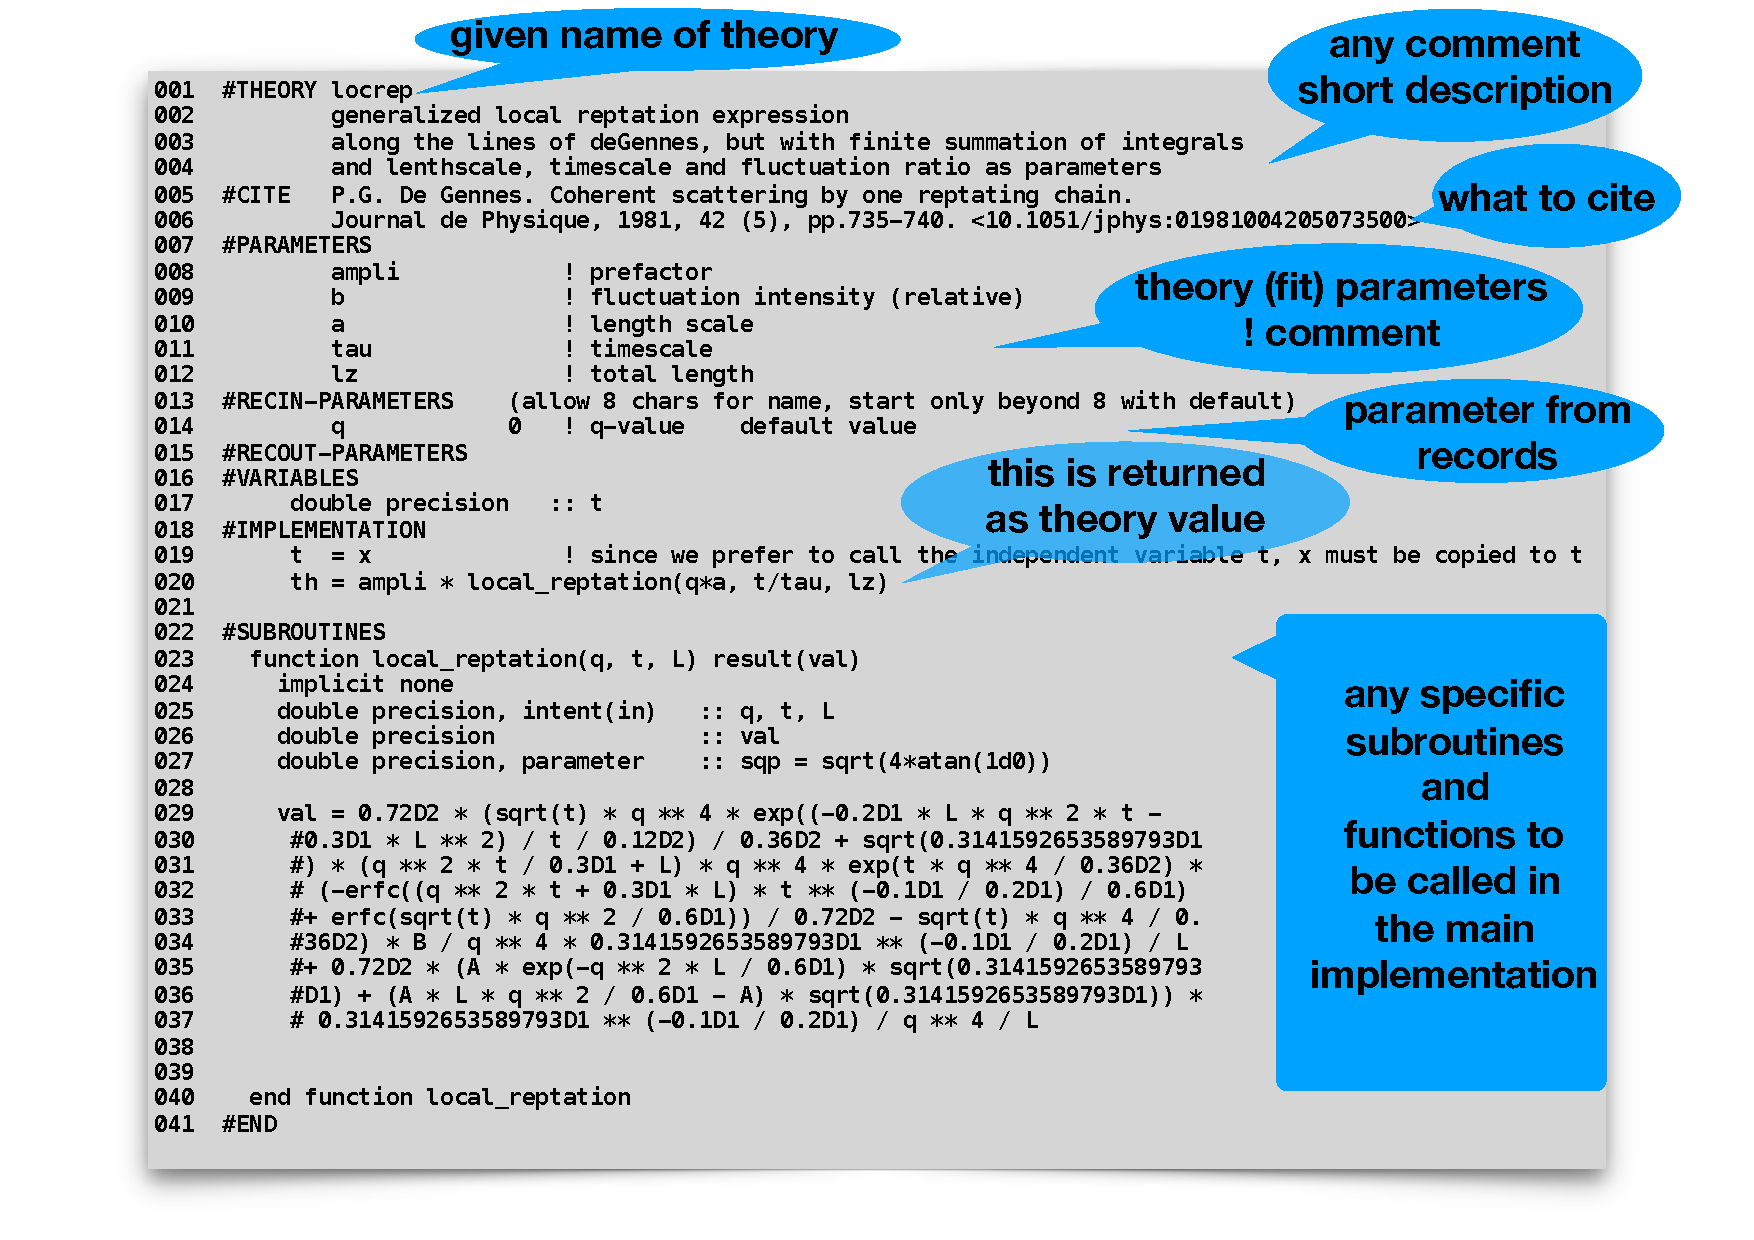
\includegraphics[width=\textwidth]{thtemplateexample.pdf}

The \#KEYWORD lines start the different input groups.

\begin{itemize}
\item line 001:  \#THEORY locrep. Give a name (here: \emph{locrep}) to the theory.
\item lines 002-004: description of the theory
\item lines 005-006: citation 
\item lines 007-012: the fit parameters, list of names  and ! explanations
\item lines 013-014: parameters associated with the data records, here q. Name default value ! Explanation.
\item line 015: output parameters that are added to the record parameter section (here empty)
\item lines 016-017: fortran variable definition for any additional variables to be used in the theory
       (not needed for parameters, they are automatically created).
\item lines 018-020: implementation: fortran code to compute the theory
\item lines 022-040: any function and subroutines that are needed to do the computation

\end{itemize}

\section{Conversion to the proper Fortran theory function} 
\label{sec:finish}

\begin{corollary}
% \sysprompt \enter{cd \emph{Myworkingdirectory}} \return \\
\sysprompt {\bf th\_template\_generator $<$ my\_new\_template} \return  \expl{processes the template to \emph{out.f90}}\\
\sysprompt {\bf cp out.f90 ../theos/th\_mynewthname.f90} \return  \expl{copy source to \emph{theos}}\\ 
\sysprompt {\bf cd ../theos} \return  \expl{change directory to \home/datreat/src/theos} \\
\sysprompt {\bf make} \return  \expl{compile} 
\end{corollary}
..in most cases some residual fortran (syntax) errors will pop up (or not?!), in that case
edit the file  {\it \home/datreat/src/theos/th\_mynewthname.f90}, correct it and try
\emph{make} again until no error messages remain (see HINTS for strategies to avoid errors!).
The theory inclusion into {\bf datreat} can be finished.

\begin{corollary}
% \sysprompt \enter{cd \emph{Myworkingdirectory}} \return \\
\sysprompt {\bf make clean} \return  \expl{make sure that no old residues interfere}\\
\sysprompt {\bf make} \return  \expl{in subdirectory \emph{theos} this now compiles the theories} \\
\sysprompt {\bf cd ../} \return  \expl{change to subdirectory \emph{\home/datreat/src}} \\
\sysprompt {\bf make} \return  \expl{rebuild {\it datreat} including the new theory.} 
\end{corollary}


\section{Test and use \desc{How to use a new theory}}
\label{sec:testuse}
\index{theory (test and use of new th)}

After successful \emph{make} the new theory should be listed if datreat is started
and the commend \cmdl{th}{} is entered. \cmdl{th}{thname} then will yield the information
on parameters etc. (here thname=\emph{locrep}).
\linespace
To use it give the command \cmdl{ac}{thname} and then use \cmdl{cth}{} to enter parameter values.
Finally (after selecting some suitable record) use 
\cmdl{thc}{} to compute and then \cmdl{plot}{} and/or \cmdl{edit}{} to check the resulting values.


\section{Code Generated \desc{illustration for this example}}
\label{sec:codegen}
\index{theory (code structure)}
The above example yields the following \emph{Fortran} source code.

\tiny
\begin{verbatim}

 FUNCTION th_locrep(x, pa, thnam, parnam, npar,ini, nopar ,params,napar,mbuf)
!================================================================================
!  generalized local reptation expression along the lines of deGennes, but with finite summation of integrals and lenthscale, timescale and fluctuation ratio as parameters
!  Journal de Physique, 1981, 42 (5), pp.735-740. <10.1051/jphys:01981004205073500>
      use theory_description 
      implicit none 
      real    :: th_locrep
      character(len=8) :: thnam, parnam (*) 
      real    :: pa (*) 
      real    :: x , xh
      integer :: mbuf, nparx, ier, ini, npar, iadda
      integer, intent(inout) :: nopar       
      character(len=80), intent(inout) :: napar(mbuf) 
      real, intent(inout) :: params(mbuf) 
     
      double precision, parameter :: Pi = 4*atan(1d0)
      integer                     :: actual_record_address
     
! the internal parameter representation 
     double precision :: ampli      ! prefactor                                                                       
     double precision :: b          ! fluctuation intensity (relative)                                                
     double precision :: a          ! length scale                                                                    
     double precision :: tau        ! timescale                                                                       
     double precision :: lz         ! total length                                                                    
! the recin parameter representation 
     double precision :: q          ! q-value    default value                                                        
! the reout parameter representation 
 
     double precision :: th
 
     double precision   :: t
!
! ----- initialisation ----- 
    IF (ini.eq.0) then     
       thnam = 'locrep'
       nparx =        5
       IF (npar.lt.nparx) then
           WRITE (6,*)' theory: ',thnam,' no of parametrs=',nparx,' exceeds current max. = ',npar
          th_locrep = 0
          RETURN
       ENDIF
       npar = nparx
! >>>>> describe theory with >>>>>>> 
       idesc = next_th_desc()
       th_identifier(idesc)   = thnam
       th_explanation(idesc)  = " generalized local reptation expression along the lines of deGennes, but with finite summation of integrals and lenthscale, timescale and fluctuation ratio as parameters"
       th_citation(idesc)     = " Journal de Physique, 1981, 42 (5), pp.735-740. <10.1051/jphys:01981004205073500>"
!       --------------> set the parameter names --->
        parnam ( 1) = 'ampli   '  ! prefactor                                                                       
        parnam ( 2) = 'b       '  ! fluctuation intensity (relative)                                                
        parnam ( 3) = 'a       '  ! length scale                                                                    
        parnam ( 4) = 'tau     '  ! timescale                                                                       
        parnam ( 5) = 'lz      '  ! total length                                                                    
! >>>>> describe parameters >>>>>>> 
        th_param_desc( 1,idesc) = "prefactor" !//cr//parspace//&
        th_param_desc( 2,idesc) = "fluctuation intensity (relative)" !//cr//parspace//&
        th_param_desc( 3,idesc) = "length scale" !//cr//parspace//&
        th_param_desc( 4,idesc) = "timescale" !//cr//parspace//&
        th_param_desc( 5,idesc) = "total length" !//cr//parspace//&
! >>>>> describe record parameters used >>>>>>>
        th_file_param(:,idesc) = " " 
        th_file_param(  1,idesc) = "q        > q-value    default value"
! >>>>> describe record parameters creaqted by this theory >>>>>>> 
        th_out_param(:,idesc)  = " "
! 
        th_locrep = 0.0
 
        RETURN
     ENDIF
!
! ---- transfer parameters -----
      ampli    =      pa( 1)
      b        =      pa( 2)
      a        =      pa( 3)
      tau      =      pa( 4)
      lz       =      pa( 5)
! ---- extract parameters that are contained in the present record under consideration by fit or thc ---
      iadda = actual_record_address()
! >>> extract: q-value    default value
      xh =      0
      call parget('q       ',xh,iadda,ier)
      q        = xh
! 
! ------------------------------------------------------------------
! ----------------------- implementation ---------------------------
! ------------------------------------------------------------------
! 
     t  = x              ! since we prefer to call the independent variable t, x must be copied to t
     th = ampli * local_reptation(q*a, t/tau, lz)

     th_locrep = th
 
! ---- writing computed parameters to the record >>>  
 
 CONTAINS 
 
! subroutines and functions entered here are private to this theory and share its variables 
 
  function local_reptation(q, t, L) result(val)
    implicit none
    double precision, intent(in)   :: q, t, L
    double precision               :: val
    double precision, parameter    :: sqp = sqrt(4*atan(1d0))

    val = 0.72D2 * (sqrt(t) * q ** 4 * exp((-0.2D1 * L * q ** 2 * t -
     #0.3D1 * L ** 2) / t / 0.12D2) / 0.36D2 + sqrt(0.3141592653589793D1
     #) * (q ** 2 * t / 0.3D1 + L) * q ** 4 * exp(t * q ** 4 / 0.36D2) *
     # (-erfc((q ** 2 * t + 0.3D1 * L) * t ** (-0.1D1 / 0.2D1) / 0.6D1)
     #+ erfc(sqrt(t) * q ** 2 / 0.6D1)) / 0.72D2 - sqrt(t) * q ** 4 / 0.
     #36D2) * B / q ** 4 * 0.3141592653589793D1 ** (-0.1D1 / 0.2D1) / L
     #+ 0.72D2 * (A * exp(-q ** 2 * L / 0.6D1) * sqrt(0.3141592653589793
     #D1) + (A * L * q ** 2 / 0.6D1 - A) * sqrt(0.3141592653589793D1)) *
     # 0.3141592653589793D1 ** (-0.1D1 / 0.2D1) / q ** 4 / L


  end function local_reptation
 end function th_locrep
\end{verbatim}
\normalsize

\section{Hints \desc{How to efficiently create and debug theories}}
Debugging and verification and optimisation of a new \emph{theory} may be challenging.
The most effective approach to quickly yield reliable results is to first write
a procedure (function or subroutine) that contains the core implementation of the new
\emph{theory} on its own. To test, it is should be embedded in (or called from) a
short main program that serves for testing only.
After the \emph{theory} works satisfactory in that environment, its genuine source code
can be copied into either an appropriate \emph{template} or directly into a previously
created \emph{theory} scaffold.
 
\tiny
\begin{verbatim}

!!!!!!!!!!!!!!!!!!!!!!!!!!!!!!!!!!!!!!!!!!!!!!!!!!!!!!!!!!!!!!!!!!!!!!!!!!!!!!!!!!!
!!!  first establish a minimal test environment in terms of a main program
!!!!!!!!!!!!!!!!!!!!!!!!!!!!!!!!!!!!!!!!!!!!!!!!!!!!!!!!!!!!!!!!!!!!!!!!!!!!!!!!!!!

program testvilgi
 implicit none
 double precision :: l     = 20d0
 double precision :: wl4   = 100000d0
 double precision :: rmesh = 500
 integer          :: N     = 100

 double precision :: q, t, sqt, sqt0, sqti

 integer          :: m=10
 integer          :: i
 q = 0.05d0
 t = 0.1d0
 
 call NNvilgis(q,0d0,wl4,l,rmesh,N,sqt0)

 do i=0,m
   t = 2*i
   call NNvilgis(q,t,wl4,l,rmesh,N,sqt,sqti)
   write(*,*)q,t,sqt0,sqt/sqt0, sqti/sqt0
 enddo

CONTAINS  

!!!!!!!!!!!!!!!!!!!!!!!!!!!!!!!!!!!!!!!!!!!!!!!!!!!!!!!!!!!!!!!!!!!!!!!!!!!!!!!!!!!
!!!  here follows the genuine function to be included into the theory scaffold
!!!!!!!!!!!!!!!!!!!!!!!!!!!!!!!!!!!!!!!!!!!!!!!!!!!!!!!!!!!!!!!!!!!!!!!!!!!!!!!!!!!

 subroutine NNvilgis(q,t,wl4,l,rmesh,N,sqt, sqtint)
!==================================================
!
! Implementation of Eq. 30 of 
! [Vilgis and Boue, J. Polymer Science Part B: Polymer Physics, Vol 26, 2291-2301 (1988)]
! the Fourier integral can be done analytically an yields terms as b*exp(-a*t/(p**2+p0**2)/(p**2+p0**2)
! the p-sum is then done explicitly (efficiency increse by observing that all factors can be written as cos*
! NOTE: there are several typos in the formulae of the paper !! 
! 
  implicit none

  double precision, intent(in)  :: q        ! momentum transfer
  double precision, intent(in)  :: t        ! time
  double precision, intent(in)  :: wl4      ! rouse rate
  double precision, intent(in)  :: l        ! segment length
  double precision, intent(in)  :: rmesh    ! "confinement" length due to the harmonic potential
  integer         , intent(in)  :: N        ! number of segments (summation)
  double precision, intent(out) :: sqt      ! the sqt-value
  double precision, intent(out), optional :: sqtint      ! the sqt-value internal modes only


  double precision, parameter :: Pi = 4d0*atan(1d0)

  double precision :: coser(1:N,1:N)
  double precision :: eser(1:N)
  double precision :: rrarr(N,N)  ! just for checking can be removed later

  double precision :: p0, q0, qq0, W, pidn, rr, tt

  integer          :: nn, mm, p


  W    = wl4/l**4
  pidn = Pi / N
  q0   = l**2/(3*rmesh**2)
  p0   = q0 * N / Pi
!$OMP PARALLEL DO 
  do p=1,N
    do nn=1,N
      coser(nn,p) = cos(Pi*p*nn/dfloat(N))  / sqrt((p**2 + p0**2))
    enddo
  enddo
!$OMP END PARALLEL DO 

!$OMP PARALLEL DO 
  do p=1,N
      eser(p) = exp(-(Pi**2/N**2)*W*(p**2 + p0**2)*t)
! write(*,*)"eser:",p,t,W,(Pi**2/N**2)*W*(p**2 + p0**2),eser(p) 
  enddo
!$OMP END PARALLEL DO 

  sqt = 0
!$OMP PARALLEL DO PRIVATE(rr) REDUCTION(+:sqt)
  do nn=1,N
    do mm=1,N
      rr = 0
!$OMP PARALLEL DO REDUCTION(+:rr)
      do p=1,N
        rr = rr + coser(nn,p)**2 + coser(mm,p)**2 - 2*coser(nn,p)*coser(mm,p) * eser(p)
!        rr = rr + cos(Pi*p*nn/dfloat(N))**2/p**2 + cos(Pi*p*mm/dfloat(N))**2/p**2 - &
!                2*cos(Pi*p*nn/dfloat(N))*cos(Pi*p*mm/dfloat(N))/p**2
      enddo
!$OMP END PARALLEL DO 
      rr  = rr * 4*N / (2*Pi) /Pi 
!                              === dieser Faktor is noetig damit rr(n,m,0)=abs(n-m) 
!                              === fehlt im Paper ?!
 write(*,*)nn,mm,rr                        !! <===== THIS IS FOR DEBUGGING ONLY !!
      sqt = sqt + exp(-(q*l)**2/6d0 * rr)
      rrarr(mm,nn) = rr
    enddo
  enddo
!$OMP END PARALLEL DO 
  sqt = sqt / (N*N) 
  if(present(sqtint)) sqtint = sqt
 
! Diffusion
  qq0 = q0**2
  if(abs(W*qq0*t) > 1d-6) then
     rr     = 2*l**2/N/qq0*(1-exp(-W*qq0*t))  ! a factor of 2 different from Vilgis ...
  else
     rr     = 2*l**2*W*t/N-l**2*W**2*t**2*qq0/N
  endif

  sqt    = sqt*exp(-(q)**2/6d0 * rr)

end subroutine NNvilgis

!!!!!!!!!!!!!!!!!!!!!!!!!!!!!!!!!!!!!!!!!!!!!!!!!!!!!!!!!!!!!!!!!!!!!!!!!!!!!!!!!!!
!!!  end of the code to be copied to the final theory 
!!!  possibly after removing extra dbugging output (write...)
!!!!!!!!!!!!!!!!!!!!!!!!!!!!!!!!!!!!!!!!!!!!!!!!!!!!!!!!!!!!!!!!!!!!!!!!!!!!!!!!!!!

end program testvilgi 

\end{verbatim}
\normalsize

then with
\begin{corollary}
% \sysprompt \enter{cd \emph{Myworkingdirectory}} \return \\
\sysprompt {\bf gfortran testvilgi.f90 -fopenmp} \return  \expl{compile and build executable a.out} \\
...possibly correct syntax or other compiler errors...
\sysprompt {\bf a.out} \return  \expl{run}
\end{corollary}


% --------------------------------------------------------------------------------------------------------------
\part{Special Issues}
% --------------------------------------------------------------------------------------------------------------

\chapterimage{DatreatLogo.pdf} % Chapter heading image
\chapter{SANS and multiple scattering}

\chapterimage{DatreatLogo.pdf} % Chapter heading image
\chapter{TOF and BSS spectra}

\section{uni\_ft \desc{Fourier transform of spectra}} 
\index{uni\_ft, fourier transform of spectra}
\index{fourier transform of spectra}
\index{deconvolution, uni\_ft}
\index{resolution, uni\_ft}


\begin{exercise}
Fouriertransform of one selected spectrum from energy or frequency to the time domain. 
If one spectrum AND a resolution are
selected (observe sequence of selection!) then also the `deconvoluted'
time function is produced.
\end{exercise}


The results (fourier transforms of data and resolution as well as the
`deconvoluted' time function is found in newly created records at the
end of the list.

The algorithm is that from Reiner Zorn's uni\_ft program.

\begin{exercise}
The energy units given as x-axis are observed: {\bf micro-eV, meV, GHz, omega
( GHz)} (GHz means Giga rad/s).
\end{exercise}

First select a spectrum at second a resolution spectrum (if available/desired).
\begin{corollary}
% \sysprompt \enter{cd \emph{Myworkingdirectory}} \return \\
\dtrprompt {\bf uni\_ft} \opt{resnorm} \opt{reslim} \var{rlim} \return  \expl{fourier transform of spectrum} \\
\end{corollary}

(Further) options:
\begin{description}
\item[resnorm] if present use resolution also to normalize the result (use when cold sample is resolution!)
\item[reslim]  limit resolution deconvolution (=division) to values greater  \var{rlim}.
\item[rexpand] factor to get finer t-spacing.
\end{description}

{\bf Uni\_ft} uses the \emph{temp} parameter of the spectrum to perform a
detailed balance based symmetrising of the spectrum and the energy gain side
of the spectrum is used to (mirror) complete the energy loss side of the spectrum.
The conventions used (Marshall-Lovesey) are {\bf ${\omega > 0}$ is energy loss} of the
neutron.

% > uni_ft help
%  ==============================================================================
%  = uni_ft [store_at <n>] [resnorm]  [rexpand <val>]  [reslim <val>]            
%  =      performs fourier transform of the first selected records               
%  =      the second selected record (may) hold the resolution                   
%  =   options:                                                                  
%  =            resnorm : normalisation to resolution intensity                  
%  =            rexpand : multiplies (instead of adding)                         
%  =            reslim:   limit for resolution at deconvolution                  
%  =   spectrum x-axis unit given by valid names: micro-eV, meV, GHz, omega      
%  =   intermediate results (Ft(data), Ft(res), ..) are stored on etra records   
%  ==============================================================================

% "#####################  uni_ft ###############################################"
% "#  will use detailed balance symmetrisation: exp(",fdbf," * omega) "
% "#  assumed temperature is T =",temp," K"
% "#  a negative coeff corresponds to Marshall-Lovesey definition: "
% "#  positive omega is energy LOSS of the NEUTRON "
% "#  dt rangeexpand by factor =",range_expand,"  (cmd: uni_tf rexpand <val>) "


\chapterimage{DatreatLogo.pdf} % Chapter heading image
\chapter{NSE instrumentation/design}

\section{echocurv \desc{simulated phase scan}}
\index{echocurv}
\index{echo phase scan}
\index{phase scan echo}


\begin{exercise}
Creates phase scan intensity data that would be obtained from a NSE experiment using
a Gaussian distributed wavelength band of width ${\Delta \lambda}$ from a scatterer with
a simple relaxation with time constant ${\tau}$. 
The field integral ${J}$, and the nominal wavelength ${\lambda_0}$ determine the associated  Fourier time.

A subsequent {\bf noise} command can be use to add simulated counting noise. 
\end{exercise}


\begin{verbatim}

       if(comand.eq.'echocurv') then
!                    ---------
        if(found('help    ')) then 
           write(6,*)'=============================================================================='
           write(6,*)'= echocurv j <j> ......                                                       '
           write(6,*)'=    computation of simulated phase scan of NSE for a simple Lorenzian spect. '
           write(6,*)'=    ft by integration assuming gaussian distribution functions               '
           write(6,*)'=    parameters:                                                              '
           write(6,*)'=      j   <val>        : field integral                                      '
           write(6,*)'=      dj  <val>        : asymmetry (phase0)                                  '
           write(6,*)'=      j0delta <val>    : inhomogeneity offset (external fields..)            '
           write(6,*)'=      ddj <val>        : phase scan step (field integral)                    '
           write(6,*)'=      n <val>          : number of points in scan                            '
           write(6,*)'=      cdelta <val>     : relative inhomogeneity                              '
           write(6,*)'=      lambda0 <val>    : wavelength                                          '
           write(6,*)'=      dlambda <val>    : wavelength width                                    '
           write(6,*)'=      tau <val>        : relaxation time --> spectrum                        '
           write(6,*)'=      errabs <> errel <> maxint  : integration parameters                    '
           write(6,*)'=============================================================================='
           goto 2000
        endif



         alim(1) = alam0 - 3*dalam
         blim(1) = alam0 + 3*dalam

         alim(2) = -5.d0/tau
         blim(2) = -alim(2)



         n0 =     nech/2
         n0     = intval('n0      ',n0    ,inew)
                                                       !! aix.sp
         call     parset('n0      ',(real(n0)) ,ia1)

         nwert(ia1) = nech
         do i=1,nech
           j2echo = j1echo + (i-n0) * ddj + dj
           xwerte(i,ia1) = j2echo-j1echo
! --- imsl mehrdimensionale integration ---
           call  qand(f,2,alim,blim,erraec,errrec,maxint,               &
     &                result, errest )
           write(6,*)'result =',result,'     errest=',errest
           ywerte(i,ia1) = result
           yerror(i,ia1) = 0
         enddo
         xname(ia1) = 'dj/gm'
         yname(ia1) = 'counts'
         name(ia1)  = 'echo'
         coment(ia1)= 'echo'
         numor(ia1) = intval('numor   ',1,inew)
         

       function wlambda( alam )
!      ------------------------
! --- repraesentiert die wellenlaengenverteilung
        use wlntran
        implicit none
        real*4 arg, alam, wlambda
          arg     = ( (alam-alam0)/dalam )**2
          if(arg.lt.50.e0) then
            wlambda =  exp( -arg )
          else
            wlambda = 0.e0
          endif
       return
      END


       function sofqom( omega )
! --- repraesentiert die streufunktion, omega in s**-1
       use sqtran
       implicit none

       real*4 x, omega, sofqom
       x      = omega * tau
       sofqom = tau /(1.e0+x*x)
       return
      END


       function f(n,x)
! --- integrand ---
       use partran
       implicit none

       integer n
       real*4 x
       dimension x(n)
!
!      x(1) = lambda
!      x(2) = omega
!
! ---- larmorkonstante in rad/s/gauss
! ---- neutronenmasse durch h in 2/m/angstroem

       real*4 :: gamma=18303.33e0, xmh = 2.50607e-4, zpi = 6.283185307e0
       real*4 a,b,f,del, wlambda, sofqom
       a  = gamma*xmh*x(1)/(1.d0+xmh*x(1)*x(1)*x(2)*1d-10/zpi)
       b  = gamma*xmh*x(1)
       del= j0delta**2 + ( (j1echo+j2echo)*0.5e0*cdelta )**2
       f  = ( 1.d0 +  exp(-(a**2+b**2)*del*0.25e0 )*                    &
     &               cos( a*j1echo - b*j2echo )                         &
     &      ) * sofqom(x(2)) * wlambda(x(1))
       return
      END


 theory   echo                                                                            
      amplitu     239.9750       1.00       1.4213    
      average     242.4903       1.00       1.1182    
      derotat     0.000000       0.00       0.0000    
      lambda0     8.000000       0.00       0.0000    
      lamfwhm    0.8316469      0.100      0.18950E-01
      ishift      0.000000       0.00       0.0000    
      nturns      82.04076       1.00      0.52094E-01
      rcoil      0.3100000       0.00       0.0000    
      lcoil      0.4700000E-01   0.00       0.0000    
      acoil      -1.154000       0.00       0.0000    
      bcoil       1.700000       0.00       0.0000    
      a2coil     -3.600000       0.00       0.0000    
 theory   bkgr                                                                            
      level       0.000000       0.00       0.0000    
      slope       0.000000       0.00       0.0000    
 end
\end{verbatim}

\linespace
{\bf Note:} The presently used 2D-integration may fail in cases with very low echo or other extremes!
\tbd{Replace 2 integragtion scuhre by a better method (adapint recursive)!} 

\chapterimage{DatreatLogo.pdf} % Chapter heading image
\chapter{Development tools}

\section{noise \desc{add Gaussian noise and errors to a record}}
\index{noise, add noise to records}
\index{Gaussian noise}
\index{errors (creation)}

\begin{exercise}
After scaling the y-values by ${a}$ such that they (virtually) correspond to direct counting results
a Gaussian random variable is added to them in order to simulate counting statistics noise.
The associated errors are set accordingly. 
If the option \opt{errors} is given, only the errors are set but no noise is added to the y-values.
\end{exercise}

\linespace

All selected records are treated with the same ${a}$ and options, finally the results are on new 
records, which are selected. The noise application is notified by a new parameter \emph{noise\_a}.

\linespace

\begin{corollary}
% \sysprompt \enter{cd \emph{Myworkingdirectory}} \return \\
\dtrprompt \cmdl{noise}{a \var{${a}$} \opt{errors} \opt{iseed} \var{seed}}   \return 
\end{corollary}


\linespace
{\bf Note:} The factor ${a}$ must explicitly be specified and chosen such that it reconverts
the y-data to (virtual) counting results, i.e. $\sigma(a\,y) = \sqrt{a\,y}$.
The results may be scaled back to the original gauge by \cmdl{fxy}{x=X y=Y/noise\_a}.


% --------------------------------------------------------------------------------------------------------------
\part{Working Examples}
% --------------------------------------------------------------------------------------------------------------
\chapterimage{DatreatLogoPremak.pdf} % Chapter heading image
\chapter{Recommended workflows}
\index{workflow}

\section{Open a terminal \desc{from there datreat may be started}}
\index{terminal}
\index{start}
Datreat is command driven, in order to use it one has to open a \emph{terminal} (or a
\emph{shell} within e.g. an editor like \emph{emacs}).
On a \emph{Mac OSX} computer you may do this by typing (key)s: 
\begin{corollary}
% \sysprompt \enter{cd \emph{Myworkingdirectory}} \return \\
press: {\bf (command)+(space)} \\
type: {\bf terminal \return}
\end{corollary}
or if there is already a terminal open, click into that terminal and
\begin{corollary}
% \sysprompt \enter{cd \emph{Myworkingdirectory}} \return \\
press: {\bf (command)+n} 
\end{corollary}
and a new terminal will open.

Within that terminal switch to the desired subdirectory:
\begin{corollary}
% \sysprompt \enter{cd \emph{Myworkingdirectory}} \return \\
\sysprompt {\bf cd \home/myworkingdirectory} \return 
\end{corollary}

\linespace
{\bf Note 1:} On a Mac \emph{terminal} a protocol of a session can readily be stored by either
pressing the keys {\bf command+s} or using the \emph{shell} pull down menu and click on
\emph{text exportieren}.

\linespace
{\bf Note 2:} Datreat keeps a history file: {\bf .last\_dtr\_commands} in the working directory that allows
to repeat previous command lines by pressing the {\bf arrow}-keys /{\bf up} or {\bf down}.
The history is \emph{private} to the respective working directory and is kept between several
invocations of datreat.

\section{Directories  \desc{"where" to do the work}}
\index{working directory}
It is recommended to select/create a working directory, switch to that directory
and possibly copy the data to that directory. The latter is not mandatory.
The start datreat from that directory. 
\begin{corollary}
% \sysprompt \enter{cd \emph{Myworkingdirectory}} \return \\
\sysprompt {\bf cd \home/myworkingdirectory} \return \\ 
\sysprompt {\bf datreat}
\end{corollary}

Output, plots, command line-history and primary source of makros is THIS directory.


\chapter{Workflows: examples}
\label{cha:workex}

\section{A simple start \desc{basic usage example}}
\index{start}
\index{simple start}

To make first steps and get an idea of the datreat philosophy the following is recommended:

First create a (subdirectory) to work for this problem, copy the data file(s) to it and start \emph{datreat}
\begin{corollary}
% \sysprompt \enter{cd \emph{Myworkingdirectory}} \return \\
\sysprompt {\bf mkdir Myworkingdirectory} \return \\ 
\sysprompt {\bf cd Myworkingdirectory} \return  \\
\sysprompt {\bf cp ~/Desktop/datreat/TRAINING/DENDRIMER\_datreat/SB5q0.dtr ./}  \return \expl{copy an example data file}\\
\sysprompt {\bf datreat} \return \expl{start datreat} \\
\end{corollary}

now the datreat prompt appears and will accept datreat commands (it is further transparent for non ambiguous
shell commands).
First create a (subdirectory) to work for this problem, copy the data file(s) to it and start \emph{datreat}

\begin{corollary}
% \sysprompt \enter{cd \emph{Myworkingdirectory}} \return \\
\dtrprompt \cmdl{in}{SB5q0.dtr} \return \expl{read the data into the record memory} \\ 
\dtrprompt \cmdl{sel}{1} \return \expl{select the 1st record in memory} \\ 
\dtrprompt \cmdl{dir}{} \return \expl{check by listing the contents of record memory} \\ 
\dtrprompt \cmdl{aplot}{errors} \return \expl{autoplot (makro) with errors} \\ 
\dtrprompt \cmdl{ac}{strexpo} \return \expl{activate theory strexpo} \\ 
\dtrprompt \cmdl{cth}{} \return \expl{open theory specification for parameter editing} \\ 
\dtrprompt \cmdl{thc}{} \return \expl{first just calculate the theory to check start parameters etc.} \\ 
\dtrprompt \cmdl{plot}{ymin 0} \return \expl{using plot to examine} \\ 
\dtrprompt \cmdl{fit}{} \return \expl{now fit} \\ 
\dtrprompt \cmdl{plot}{ymin 0} \return \expl{check plot now with ymin set to 0} \\ 
\dtrprompt \cmdl{msave}{myfirstfit} \return \expl{save data fit and model} \\ 
\dtrprompt ... \\ 
\dtrprompt \cmdl{quit} \return \expl{exit datreat} 
\end{corollary}

To resume work you may simply use:
\begin{corollary}
\sysprompt {\bf datreat} \return \expl{start datreat and restores last state} \\
% \sysprompt \enter{cd \emph{Myworkingdirectory}} \return \\
\dtrprompt ... \\ 
\dtrprompt \cmdl{quit} \return \expl{exit datreat} 
\end{corollary}
\begin{corollary}
\sysprompt {\bf datreat 0} \return \expl{start datreat without restoring} \\
% \sysprompt \enter{cd \emph{Myworkingdirectory}} \return \\
\dtrprompt \cmdl{inplus}{myfirstfit} \return \expl{read save data and fit into} \\ 
\dtrprompt \cmdl{sel}{1} \return \expl{select the 1st record in memory} \\ 
\dtrprompt \cmdl{dir}{} \return \expl{check by listing the contents of record memory} \\ 
\dtrprompt ... \\ 
\dtrprompt \cmdl{quit} \return \expl{exit datreat} 
\end{corollary}

\section{Automation and makros \desc{prepmak: a more complex makro example}}
\index{makro, example}
\index{prepmak, makro example}
\index{automation and makros}
As example we examine the \emph{makro} {\bf prepmak}, which is used in the TRAINING/DENDRIMER context
to prepare consolidated data for datreat from a certain set of raw data.
To invoke it:
\begin{corollary}
% \sysprompt \enter{cd \emph{Myworkingdirectory}} \return \\
\dtrprompt \cmdl{prepmak}{0.1} \return \expl{makro call preparing, scaling and averaging SANS data}
\end{corollary}

\linespace

{\bf The makro, Preliminaries:}
\begin{corollary}
% \sysprompt \enter{cd \emph{Myworkingdirectory}} \return \\
1 {\bf makro \_x\_ }  \expl{first line telling it is a makro with one argument \_x\_} \\
2 \\
3 {\bf set xc (\_x\_)} \expl{store argument value to variable \emph{xc}} \\
4 {\bf ?? (xc) } \expl{show value of \emph{xc} (for check only)}
\end{corollary}

next define some preset variables, if change is needed it can be done here.

\begin{corollary}
% \sysprompt \enter{cd \emph{Myworkingdirectory}} \return \\
5 {\bf set clp1 8 }  \expl{set var \emph{clp1} to 8 } \\
6 {\bf set clp2 20 }  \expl{set var \emph{clp2} to 20} \\
7 \\
8 {\bf set xfit1 0.002} \expl{set \emph{xfit1} to 0.002 } \\
9 {\bf set xfit2 0.25 } \expl{set \emph{xfit2} to 0.25}
10 {\bf vars? } \expl{display all variables for (check only)}
\end{corollary}

here we set variables for clipping \emph{clp1, clp2} and fit range \emph{xfit1,2}.

\begin{corollary}
% \sysprompt \enter{cd \emph{Myworkingdirectory}} \return \\
11 {\bf ! run the collecting and transform of data (shell script)} \\
12 {\bf sys cotxtdtr} \expl{run shell script on the operating system level}
\end{corollary}
This is an example how data preparations beyond the scope of datreat commands
may be included. {\bf cotxtdtr} is the name of a specific shell script that 
(in this example) contains calls of data-conversion routines to prepare
datreat compatible data formats for the here treated data. At the end the
\emph{datreat input file} {\bf eqsans\_dendrimer} is written. In the following course
of the makros it will be read using the datreat command {\bf in}.

More details on \emph{cotxtdtr} will be given below.

But for now we proceed with the proper makro.

\begin{corollary}
% \sysprompt \enter{cd \emph{Myworkingdirectory}} \return \\
14 {\bf purge all} \expl{clear the record memory completely} \\
15 {\bf in eqsans\_dendrimer} \expl{read the data} \\
16 {\bf dir} \expl{list the contents of the record memory} 
\end{corollary}

Now SANS data for different detector distances with different scales and for different samples 
as was converted and written to the datreat output file \emph{eqsans\_dendrimer} (and augmented by auxiliary information) by running \emph{cotxtdtr}, after reading using the command {\bf in},
occupies a number of records in the memory. 

\linespace

\begin{corollary}
% \sysprompt \enter{cd \emph{Myworkingdirectory}} \return \\
17 {\bf set naly 0} \expl{create and initialise a user variable naly} \\
18 {\bf set fak 0} \expl{ " fak = factor} \\
18 {\bf set ofs 0} \expl{ " ofs = offset} \\
19 {\bf set fakq 0} \expl{ " fakq } \\
21 {\bf set ofsq 0} \expl{ " ofsq } \\
22 \\
23  {\bf set irun -1} \expl{ " irun = run index variable } \\
24
\end{corollary}
Here a number of user defined variables (chosen names) are initialised. They serve to
determine averages and variances for the linear scaling parameters \emph{fak, ofs} used to align 
data from the two detector distance.
Finally a counter/pointer to the records to be processed (\emph{irun}) is set.

\linespace
Now the first pair of records is processed:
\begin{corollary}
% \sysprompt \enter{cd \emph{Myworkingdirectory}} \return \\
26 ! treat first pair of detector distances
27 {\bf set irun (irun+2)}  \expl{increment record counter} \\
28 {\bf sel (irun)}  \expl{select first record of this pair} \\ 
29 {\bf clip from 1 to (clp1)} \expl{remove the first clp points (beam stop)$^1$} \\ 
30 {\bf sel (irun+1)}  \expl{select the other record of this pair} \\ 
31 {\bf clip from (nv(irun+1)-clp2) to nv(irun+1)} \expl{remove the last clp2 points$^2$} \\
32 {\bf sel (irun) (irun+1)} \expl{select both (now clipped) records} \\ 
33 {\bf set nn (num(isel(1)))} \expl{remember the numor of the first selected record} \\
34 {\bf aligny } \expl{use overlap between selected records for scaling} \\
35 {\bf set naly (naly+1)} \expl{count the number of scaling actions} \\
36 {\bf set fak  (fak+aligny\_s)} \expl{add the present factor aligny\_s to fak} \\
37 {\bf set ofs  (ofs+aligny\_o)} \expl{same for offset} \\
38 {\bf set fakq  (fakq+aligny\_s\^2)} \expl{..and collect squares for the variances} \\
39 {\bf set ofsq  (ofsq+aligny\_o\^2)} \expl{"} \\
40 {\bf average xcatch (xc)} \expl{finally average and combine the two scaled records} \\
41 {\bf putpar avof (nn)} \expl{put information of the original numor to the average}
\end{corollary}

$^1$ the variable \emph{clp1} was set in line 6 of the macro, note the \emph{clip} acts 
on place.

$^2$ the variable \emph{clp2} was set in line 6 of the macro, note the \emph{clip} acts 
on place.

\linespace
This now is repeated for all present pairs of detector distance data.
Thus the sequence an number is \emph{customized} to the available data for this
measurement.
\begin{corollary}
% \sysprompt \enter{cd \emph{Myworkingdirectory}} \return \\
43 ! sel 3 4 \\
44 {\bf set irun (irun+2)}  \expl{increment record counter} \\
...
...
\end{corollary}

Then we do final adjustments to the parameters etc. and store the consolidated
results.

\begin{corollary}
218 {\bf sel all avof 2000 band 4000} \expl{now all results that have the parameter avof are selected} \\
219 {\bf rename xaxis \verb! $$\rm\bf~q\,~\slash~\,\AA{^-1}! } \expl{tex-style "pretty" x-axis}\\
220 {\bf rename yaxis  I(q)/[a.u.]} \expl{y-axis name} \\
221 \\
222 {\bf p0 xmin 0.001 xmax 1 ymin 0.01 ymax 10 log\_x log\_y colo 0 1 2 3 4 5 6 7 8 9 errors} 
\expl{prepare plot} \\
223 \\
224 {\bf set fak  (fak/naly) } \expl{normalise averages ...}\\
225 {\bf set ofs  (ofs/naly) } \expl{  " }\\
226 {\bf set fakq (sqrt(fakq/naly-fak*fak))} \expl{... and compute variances } \\
227 {\bf set ofsq (sqrt(ofsq/naly-ofs*ofs))} \expl{  " }\\
228 {\bf putpar fakq (fakq) } \expl{..and put the results to the parameters of the records}\\
229 {\bf putpar fak  (fak)} \expl{ " } \\
230 {\bf putpar ofsq (ofsq)} \expl{ " }  \\
231 {\bf putpar ofs  (ofs)} \expl{ " }  \\
232 {\bf msave allsansav } \expl{store (all) final result records to file allsansav}\\
233 {\bf purge all} \expl{clear record memory}\\
234 {\bf in allsansav } \expl{read the final records in a cleared memory, i.e from position 1}
\end{corollary}

So now the data are prepared for further analysis, e.g. {\bf fitting}.
So first we set up a model, here: background ({\bf bkgr}) + extended Debye model with A2 and discrete
summation with fractal chain expansion ({\bf ndebye}).

\begin{corollary}
242 {\bf dac} \expl{clear any previous model definitions} \\
243 {\bf ac bkgr} \expl{add one background model instance} \\
243 {\bf ac ndebye} \expl{add one Debye model instance} \\
244 \\
245 {\bf chgthpar ndebye 1 ampli    par    0.01        scale  0.01} \expl{set start parameters ...}   \\ 
246 {\bf chgthpar ndebye 1 n        par   333          scale  0.00     ! do not fit ! }   \\
247 {\bf chgthpar ndebye 1 l        par    10          scale  0.100 } \\    
248 {\bf chgthpar ndebye 1 nu       par    0.4         scale  0.100 } \\    
249 {\bf chgthpar ndebye 1 chi      par    1e-3        scale  1e-3  } \\   
250 {\bf chgthpar ndebye 1 withsq   par    1           scale  0.0   } \\ 
251 \\
252 {\bf al} \expl{finally display the model setting (and write lastth)}
\end{corollary}

Now we are ready for some fitting:

\begin{corollary}
257 !  fit and determine background
258 {\bf set nn (nbuf)} \expl{put number of datasets (records) to nn} \\
259 {\bf set i 1} \expl{initialize loop counter} \\
260 {\bf :j1}  \expl{label (loop start)}\\
261 {\bf sel (i)} \expl{select i-th record  }
262 {\bf rename xaxis \verb! $$\rm\bf~q\,~\slash~\,\AA{^-1}! } \expl{tex-style "pretty" x-axis}\\
263 {\bf rename yaxis  I(q)/[a.u.]} \expl{y-axis name} \\
264 {\bf  fit x1 (xfit1) x2 (xfit2)} \expl{do the fitting for record i} \\
265 {\bf  thc n -200 x1 0.001 x2 0.5} \expl{compute fit result over the extended q-range} \\
266 {\bf  plot \# 1} \expl{...and plot this} \\
267 {\bf fun y+ (-level)}$^1$ \expl{subtract the fitted background level} \\
268 {\bf putpar bgrsub (level) } \expl{and add the (subtracted) level to the parameters} \\
267 {\bf plot} \expl{plot the background subtracted version} \\
268 {\bf set i (i+1)} \expl{increment the (intended) loop index} \\
269 {\bf if (i) $<=$ (nn) then goto :j1} \expl{jump to loop start if i $\le$ nn}
\end{corollary}

...the loop serve mainly as illustration here, usually fitting is done more interactively.

\subsection{The shell script cotxtdtr}
\label{ssec:cotxtdtr}
\index{cotxtdtr}
\index{data conversion example}
\index{shell script}
\index{fortran}
\index{rp.f90}
In the above example makro we use the shell script \emph{cotxtdtr} called by the command
\cmdl{sys}{cotxtdtr}. The name is freely chosen (here meaning {\bf co}nvert{\bf txt}to{\bf dtr}).
The explicit use of {\bf sys} ensures that the name is not mixed up with any \emph{makro} 
or \emph{genuine datreat command}.

\rule{6cm}{1pt} cotxtdtr \rule{6cm}{1pt} 
%
\footnotesize
\begin{verbatim}
 1: gfortran rp.f90
 2: a.out sHB2_1o3m.txt   0.020  1.03  3021 >   eqsans_denrimer      
 3: a.out sHB2_4o5m.txt   0.020  4.05  3022 >>  eqsans_denrimer      
 4: a.out sHB3p5_1o3m.txt 0.035  1.03  3031 >>  eqsans_denrimer        
 5: a.out sHB3p5_4o5m.txt 0.035  4.05  3032 >>  eqsans_denrimer        
 6: a.out sHB5_1o3m.txt   0.050  1.03  3051 >>  eqsans_denrimer      
 7: a.out sHB5_4o5m.txt   0.050  4.05  3052 >>  eqsans_denrimer      
 8: a.out sL2_1o3m.txt    0.020  1.03  1021 >>  eqsans_denrimer     
 9: a.out sL2_4o5m.txt    0.020  4.05  1022 >>  eqsans_denrimer     
10: a.out sL3p5_1o3m.txt  0.035  1.03  1031 >>  eqsans_denrimer       
11: a.out sL3p5_4o5m.txt  0.035  4.05  1032 >>  eqsans_denrimer       
12: a.out sL5_1o3m.txt    0.050  1.03  1051 >>  eqsans_denrimer     
13: a.out sL5_4o5m.txt    0.050  4.05  1052 >>  eqsans_denrimer     
14: a.out sSB2_1o3m.txt   0.020  1.03  2021 >>  eqsans_denrimer      
15: a.out sSB2_4o5m.txt   0.020  4.05  2022 >>  eqsans_denrimer      
16: a.out sSB3p5_1o3m.txt 0.030  1.03  2031 >>  eqsans_denrimer        
17: a.out sSB3p5_4o5m.txt 0.030  4.05  2032 >>  eqsans_denrimer        
18: a.out sSB5_1o3m.txt   0.050  1.03  2051 >>  eqsans_denrimer      
19: a.out sSB5_4o5m.txt   0.050  4.05  2052 >>  eqsans_denrimer   
20: cat L1.dat    >>    eqsans_denrimer   
21: cat L10.dat   >>    eqsans_denrimer   
22: # cat S1.dat    >>    eqsans_denrimer   
23: # cat S10.dat   >>    eqsans_denrimer   
24: cat HB1.dat   >>    eqsans_denrimer   
25: cat HB10.dat  >>    eqsans_denrimer   
\end{verbatim}
\normalsize
%
%\rule{6cm}{1pt}\rule{\widthof{ cotxtdtr }}{1pt}\rule{6cm}{1pt}
\rule{12cm+\widthof{ cotxtdtr }}{1pt}

The intention of this shell-script is to convert raw data that come in a different form 
(files \emph{*.txt}) to datreat format and at this occasion include further missing metadata.
The results in datreat format are all collected in one single file: \emph{eqsans\_denrimer}.
The method chosen to do this here is to use a custom written small fortran program {\bf rp.f90}
to perform the task. Besides the raw file names it also accepts further metadata numbers
enabling to put ${q}$, detector distance and a given id-number (numor).
The program  {\bf rp.f90} is freshly compiled in line 1. The compiler call in this form
creates an executable {\bf a.out}, which in the following lines is called to do the conversion.
The UNIX redirection operators \verb! > ! (write output to file) and \verb! >> ! (append output to
file) are used to push the converted data to the target file \emph{eqsans\_denrimer}.
Finally in lines 20: - 25: the UNIX \emph{cat} command is used to also append some data that are
already present in datreat format.

\linespace

\rule{6cm}{1pt} rp.f90 \rule{6cm}{1pt} 
%
\tiny
\begin{verbatim}

! read SANS DATA: 
! use gfortran rp.f90
! a.out filename <conc> <collen> <numor> > datfile
program rp
implicit none
double precision :: q, iq, err, dx, conc, l2
integer          :: ios
integer          :: numor
CHARACTER(len=255) :: cmd, lin, fil

     CALL get_command_argument(1,fil)  ! the first argument (to a.out) is the filename
     open(10, file=trim (fil))         ! open the file
     CALL get_command_argument(2,cmd)  ! the next argument holds the concentration
     read(cmd,*) conc                  ! convert the concentration from string to number
     CALL get_command_argument(3,cmd)  ! the next argument is the detectro distance l2
     read(cmd,*) l2                    ! convert it to a number
     CALL get_command_argument(4,cmd)  ! the last (4-th) argument is the numot
     read(cmd,*) numor                 ! convert it to a number
     write(*,'(a)')trim(fil)                                ! write filename as comment to *=stdout (> eqsans_denrimer)
     write(*,'(a,a,i9)')fil(1:8),'  "I(q)"  vs q  ', numor  ! write the "versus" line for datreat
     write(*,'(a,f12.6)') "conc ", conc                     ! put parameter conc
     write(*,'(a,f12.6)') "l2 ", l2                         ! put parameter l2
     write(*,*)"values"                                     ! optional values indicator
     do                                                     ! loop over lines in txt-file
       read(10,'(a)',iostat=ios)lin                           ! read a line
       if(ios .ne.0 ) exit                                    ! exit=finish if no longer successful
       read(lin,*,iostat=ios) q, iq, err, dx                  ! convert to numbers
       if(ios .ne. 0) cycle                                   ! skip if conversion did not succeed
       if(iq  == 0d0) cycle                                   ! skip if inensity (empty data)
       write(*,'(3f14.7)') q, iq, err                         ! write q, intensity and error to stdout
     enddo                                                  ! end of loop
     write(*,'(a)')"#nxt"                                   ! write a end group label 
     close(10)
end program rp 
\end{verbatim}
\normalsize
%
%\rule{6cm}{1pt}\rule{\widthof{ cotxtdtr }}{1pt}\rule{6cm}{1pt}
\rule{12cm+\widthof{ rp.f90 }}{1pt}

\linespace

Used to read data in the form:

\rule{5cm}{1pt} sHB2\_1o3m.txt  \rule{5cm}{1pt} 
%
\footnotesize
\begin{verbatim}
# X , Y , E , DX
1
0.00533729,0,0,0.00140787
0.0105999,2.62143,0.0200395,0.00296718
0.0158626,2.53719,0.00987976,0.00307715
0.0211252,2.40522,0.00751643,0.0030474
0.0263878,2.28613,0.005733,0.00309758
0.0316505,2.13021,0.00480097,0.0031552
...
...
...
0.763157,0.168901,0.0193701,0.0215116
0.76842,0.142007,0.0259377,0.0216196
0.773683,0.17035,0.0376949,0.0108332
0.778945,0,0,0
0.784208,0,0,0
0.789471,0,0,0
\end{verbatim}
\normalsize
%
%\rule{6cm}{1pt}\rule{\widthof{ cotxtdtr }}{1pt}\rule{6cm}{1pt}
\rule{10cm+\widthof{ sHB2\_1o3m.txt  }}{1pt}


% --------------------------------------------------------------------------------------------------------------
\part{Theories}
%  anisodi   beaucage  benoitmf  bkgr      d2sphere  ddiavo    debstar   debye2  
%  degenne2  degennea  degennes  diffusio  dirosp    dolgushe  echo      echotri2
%  eval      gauss     gauss2    gaussft   hetdif    hetdifq   hyperbra  kohl_q  
%  kohlfast  likhtman  ln_bss1   locrep    locrep2   locrep3   lrep2nr   moderato
%  ndebye    ndendpy   ndendri   nmrdiff   nmrdiff2  nmrdiff3  nnvilgis  nrouconf
%  nrous_22  nrous_s2  nrous_s4  nrousefn  nrousefy  nrousep   nrouserr  nvilgis 
%  nzimm_pn  nzimm_s   nzimmaz   peryev    q**n      repmode2  riggch    ring2   
%  ring2a    ring2b    roufbead  rouse     rpalin    rparing   rpastar2  rpastar3
%  sansfac   shell3_f  sinhafra  sofq      srouse    star      strexpo   strexpsq
%  strexsqq  thickco2  thickco4  zgbic2    zglam1    zimm    

\chapterimage{DatreatLogo.pdf} % Chapter heading image
\chapter{strexpo \desc{generic streched exponential}}
\index{strexpo}


\begin{exercise}
\begin{equation}
f_{th}(x=t;\{q\}) = A \, \exp \left (
- \left [ \frac{|t|}{\tau_0 q^n}
 \right ]^\beta
 \right )
\end{equation}
\end{exercise}

\linespace

Direct theory parameters ( (fit)parameters in model definition ):
\begin{tabbing}
\textbf{keyword-----}  \= command name, it is the first item of the command \= pretreat   \=   \kill
\textbf{Parameter}  \> meaning                                           \> pretreat   \> fit      \\
\textbf{amplitu  } \>  $A$, standard pre factor                           \>  --        \> yes      \\         
\textbf{tau      } \>  $\tau_0$ time constant                            \> $|\cdots|$ \> yes      \\
\textbf{beta     } \>  $\beta$  stretching exponent                       \> $|\cdots|$ \> yes       \\
\textbf{qexp     } \>  $n$ exponent of q-dependence                      \>  --        \> yes      \\   
\end{tabbing}

\linespace
Used record parameters: 
\begin{tabbing}
\textbf{keyword--}  \= command name, it is the first item of the command line                    \kill
\textbf{q        } \>  $q$, q-value for this record          \\         
\end{tabbing}

\linespace
Parameters pushed to records:
\begin{tabbing}
\textbf{keyword--}  \= command name, it is the first item of the command line                    \kill
\textbf{tauave0  } \>  $\tau_0  \Gamma(1\beta) /\beta$, average tau           \\         
\textbf{tauave  }  \>  $\tau    \Gamma(1\beta) /\beta$, average tau(q)       \\         
\textbf{deff    }  \>  $1 /[q^2 \tau    \Gamma(1\beta) /\beta]$, effective diffusion      \\         
\end{tabbing}

\linespace
{\bf Note:} Fix $n=0$ \emph{(qexp)} to get a simple, q-independent stretched exponential!

\chapter{gauss, gauss2, gaussft \desc{Gaussians}}
\index{gauss}
\index{gauss2}
\index{gaussft}

\begin{exercise}
\textbf{gauss} : \expl{plain Gaussian}\\
\begin{equation}
f_{th}(x) = A \, \exp \left (
- \left [ \frac{x-x_0}{w}
 \right ]^2
 \right )
\end{equation}
\end{exercise}

\linespace


Direct theory parameters ( (fit)parameters in model definition ):
\begin{tabbing}
\textbf{keyword-----}  \= command name, it is the first item of the command \= pretreat   \=   \kill
\textbf{Parameter}  \> meaning                                           \> pretreat   \> fit      \\
\textbf{intensit  } \>  $A$, standard pre factor                          \>  --        \> yes      \\         
\textbf{width     } \>  $w = \sqrt{2} \sigma$, width                     \> --        \> yes      \\
\textbf{center    } \>  $x_0$, center                                    \> --        \> yes       \\
\end{tabbing}

\linespace
Used record parameters: 
\begin{tabbing}
\textbf{keyword--}  \= command name, it is the first item of the command line                    \kill
\textbf{-none-   } \>            \\         
\end{tabbing}

\linespace
Parameters pushed to records:
\begin{tabbing}
\textbf{keyword--}  \= command name, it is the first item of the command line                    \kill
\textbf{-none-  } \>            \\         
\end{tabbing}

\linespace
{\bf Note:} this function is intended to accurately model (resolution) contribution with
width in the range or smaller than the bin-width of histogramed data.


\begin{exercise}
\textbf{gauss2} : \expl{Gaussian integrated over (one fixed) channel-width}\\
\begin{equation}
f_{th}(x) = A \, 
(\sqrt{\pi/4} w/\Delta x)) 
\left (\mathrm{erf} \left [\frac{2(x-x_0)+\Delta x}{2 \Delta x} \right ]-
\mathrm{erf} \left [\frac{2 (x-x_0)-\Delta x}{2 \Delta x
} \right ] \right )
\end{equation}
\end{exercise}


Direct theory parameters ( (fit)parameters in model definition ):
\begin{tabbing}
\textbf{keyword-----}  \= command name, it is the first item of the command \= pretreat   \=   \kill
\textbf{Parameter}  \> meaning                                           \> pretreat   \> fit      \\
\textbf{intensit  } \>  $A$, standard pre factor                          \>  --        \> yes      \\         
\textbf{width     } \>  $w = \sqrt{2} \sigma$, width                     \> --        \> yes      \\
\textbf{center    } \>  $x_0$, center                                    \> --        \> yes       \\
\textbf{xbinwid   } \>  $\Delta_x$ channel width                         \> --        \> no       \\
\end{tabbing}

\linespace
Used record parameters: 
\begin{tabbing}
\textbf{keyword--}  \= command name, it is the first item of the command line                    \kill
\textbf{-none-   } \>            \\         
\end{tabbing}

\linespace
Parameters pushed to records:
\begin{tabbing}
\textbf{keyword--}  \= command name, it is the first item of the command line                    \kill
\textbf{-none-  } \>            \\         
\end{tabbing}

\linespace

\begin{exercise}
\textbf{gaussft} : \expl{Gaussian for resolution model ?OBSOLETE?}\\
\end{exercise}

\chapter{Spectral functions in ${\omega}$ \desc{General aspects for resolution broadened spectra.}}
\index{spectra}
\index{resolution convolution}
Resolution convolution is performed by multiplication of the intermediate scattering function with the
Fourier transform of the resolution function. This Fourier transform is obtained by using a representation 
of the resolution function in terms of Gaussians
\begin{equation}
\label{eg:gares}
{\cal R}(Q,\omega) = \sum_{i=1}^{N} { a_i \, e^{-(\omega-\omega_i)^2/w_i^2} }
\end{equation}
with the Fourier-representation
\begin{equation}
\label{eg:garesF}
{\cal R}(Q,\omega) = \sum_{i=1}^{N} {\int \frac{a_i \, e^{-(w_i \, t)^2/4}}{ 2 \pi^{3/2} \, w_i }\, \cos([\omega-\omega_i]\,t) d\omega}
\end{equation}
typically the components of the Gaussian representations have a rather limited extension in
the time domain such that the numerical Fouriertransform of the product with the intermediate
scattering function can be restricted to a corresponding maximum time, thus yielding an 
efficient computation of the expected experimentally observed spectrum
\begin{equation}
\label{eq:conv1}
I(Q,\omega) = \sum_{i=1}^{N} { \int_0^{t_{\max} = W_t/w_i} {
\frac{a_i \, e^{-(w_i \, t)^2/4}}{ 2 \pi^{3/2} \, w_i } \, \cos([\omega-\omega_i]\, t) \, S(Q,t) \, dt 
}}
\end{equation}
where the coefficient $W_t$ used for the upper time limit is selected such that the integral
contributions beyond that point are sufficiently reduced, here a value of 5 is used sich that
the integrand is reduced with a factor of less than $2 \times 10^{-3}$ due to the resolution
factor (if reqired the factor may easily be increased without causing too much extra computational effort). 
The procedure as outline above captures the salient features use for fitting the results,
however, to cope with effects pertaining to the finite width of one energy/frequency bin
$\Delta \omega$, which will play a role if broadening effects in the range of $\Delta \omega$
are to be considered, the final form of the method takes account for these effects by the
following modifications.
1. the resolution is fitted with the integral of the Gaussian over the channel width 
%
\begin{equation} 
\sum_{i=1}^{N} { a_i \{ \sqrt{\pi/4}\, w_i/\Delta \omega \} \,(
{\rm erf}([2\omega+\Delta \omega]/2w_i)-{\rm erf}([2\omega-\Delta\omega]/2w_i)) 
}
\end{equation}
.

2. when computing the estimation of the measured intensity $I(Q,\omega)$ the same
integration over a channel width is performed, which effectively is achieved by
replacing Eq. \ref{eq:conv1} by
\begin{equation}
\label{eq:conv1}
I(Q,\omega) = \sum_{i=1}^{N} { \int_0^{t_{\max} = W_t/w_i} {
\frac{a_i \, e^{-(w_i \, t)^2/4}}{ 2 \pi^{3/2} \, w_i } \, 
\frac{ 
\sin(\{-[\omega-\omega_i]+\Delta\omega/2\}\, t)+\sin(\}[\omega-\omega_i]+\Delta\omega/2\}\, t)
}{
t \, \Delta\omega
} 
\, S(Q,t) \, dt 
}}
\end{equation}
This ensures proper treatment of spectral features with variations within the 
bin width of the histogramm of count results. For virtually any conceivable model for the
intermediate scattering function $S(Q,t)$ the numerical integration using an adaptive
method is reliable and fast. Due to the inclusion of the resolution convolution any
cutoff effects are avoided as well as the typical artefacts of replacing the integration 
by an FFT sum. 

\linespace

\begin{exercise}
The resolution parameters ${a_i}$, ${w_i}$, and ${\omega_i}$ for ${i=1 \cdots N}$ (${N \le 8}$) 
have to be determined from a suitable resolution experiment (e.g. the vvery cold sample) and
then set a parameters in the data records in order to be available the spectrum fit-theories.
\end{exercise}

\begin{tabbing}
\textbf{keyword-----}  \= command name, it is the first item of the command   \kill
\textbf{Parameter}  \> meaning                                              \\
\textbf{ga1inten  } \>  $a_1$, amplitude of first Gaussina resolution component    \\         
\textbf{ga1width  } \>  $w_1$, width of first Gaussina resolution component    \\         
\textbf{ga1center  }\>  $\omega_1$, center of first Gaussina resolution component    \\         
\textbf{...  }\>  ...    \\         
\textbf{...  }\>  ...    \\         
\textbf{ga8inten  } \>  $a_1$, amplitude of first Gaussina resolution component    \\         
\textbf{ga8width  } \>  $w_1$, width of first Gaussina resolution component    \\         
\textbf{ga8center  }\>  $\omega_1$, center of first Gaussina resolution component    \\ 
\end{tabbing}

{\bf Note:} One may specifiy less than 8 gaussian components, however, 8 is the maximum.


\section{Determination of Gaussian resolution parameters}
\index{ga1inten}
\index{ga1width}
\index{ga1center}
\index{resolution parameters}

\tbd{device more automatic procedure!}


Examples for the resolution determinetion and data preparation are found
in the makros: {\bf makres..}, {\bf getres..} and {\bf putres..}.

\tiny
{\bf makresm8}
\begin{verbatim}

makro _q_ 

! Makro for bulk PEP TOFTOF 

purge all

set n_container +nbuf
 in EmptyCan135k.i96.dat

c in EmptyCan45k.i96.dat

set n_res +nbuf
 in b10k135.i96.dat

c in b10k45.i96.dat

sel +n_res+1

sel next q (_q_) band 0.001

set n_data_s (sel)

c goto :ex

c
c subtract empty container from resolution
c

sel 0

sel next q (_q_)
sel next q (_q_) add
c goto :ex
set result (sel)

if +nsel = 2 then goto :ok0

echo "NO DATA WITH THAT Q FOUND"
goto :ex

:ok0

sel 0
sel next q (_q_)
sel next q (_q_)
sel add (result)

dsl

arit f1 1 f2 -1  to 101235

c msave file1

xformel ;(xx*1000*1.5193)
yformel ;(yy)
funfun immediate op
rename xaxis GHz


c plot xmin -1000 xmax 1000 ymin 0.001 ymax 5000 log_y

c goto :ex

c
c do the 4G + bgr resolution fitting
c
c 
c Sichern des letzten Theoriesettings auf lastth_x

c goto :ex
c
c 
c
c dummy action to set the range of peak detection as [x1,x2]
c dac
 ac bkgr
 chgthpar bkgr 1 level  par 1  scale 1
 fit x1 -1000 x2 1000 go
c
c
c
c
c In der (neuen) Datreat Version sind maxy, centerx, widthx  
c "Extract" variablen, die das Maximum und den "Schwerpunkt" und Weite (in [x1,x2])
c  der Daten des selktierten Records enthalten. Damit kann man gute Startwerte fuer den
c  Gaussian Fit finden.
c
set ym (maxy)13
set xc -centerx
set w1 +widthx
set w2 +w1*1.5
c
c
c leeren der Theorieliste und aktivierenm von 2 Gaussians
c
dac
ac gauss
ac gauss

c
c Inline Setzten von Parametern (interaktiv mit cth).
c

chgthpar gauss 1 intensit  par 1*ym        scale 1
chgthpar gauss 1 width     par +w1         scale 0
chgthpar gauss 1 center    par 0-xc        scale 0

chgthpar gauss 2 intensit  par 0.2*ym     scale 1
chgthpar gauss 2 width     par +w2        scale 0
chgthpar gauss 2 center    par 0-xc       scale 0


c
c Fit in einem eingeschraenkten Bereich um den Peak
c

fit x1 -5*w1 x2 5*w1 go
set  ssqfit1 +ssq

c
c Jetzt folgt im Wechselspiel von Parameter setzen/freigeben und
c Hinzufuegen weitere Gaussians oder background definitionen der 
c Aufbau und (hoffentlich) robuste Fit des Aufloesungsmodells 
c


chgthpar gauss 1 width     par +w1      scale 0
chgthpar gauss 2 width     par +w2      scale 0




fit 
set  ssqfit2 +ssq


chgthpar gauss 1 center    par 0-xc        scale 0
chgthpar gauss 2 center    par 0-xc        scale 0



fit 
set  ssqfit3 +ssq



c ac gauss
c chgthpar gauss 3 intensit  par 0.1*ym           scale 1
c chgthpar gauss 3 width     par (ga1width)/2     scale 0
c chgthpar gauss 3 center    par (ga1center)      scale 0


fit 
set  ssqfit4 +ssq

c chgthpar gauss 3 width     par (ga1width)/2     scale 1


fit 
set  ssqfit5 +ssq

c if +plotyes = 0 then plot

chgthpar gauss 1 intensit  par (ga1inten)        scale 1
chgthpar gauss 1 width     par (ga1width)        scale 0
chgthpar gauss 1 center    par (ga1cente)        scale 0

chgthpar gauss 2 intensit  par (ga2inten)        scale 1
chgthpar gauss 2 width     par (ga2width)        scale 0
chgthpar gauss 2 center    par (ga2cente)        scale 0

c chgthpar gauss 3 intensit  par (ga3inten)        scale 1
c chgthpar gauss 3 width     par (ga3width)        scale 0
c chgthpar gauss 3 center    par (ga3cente)        scale 0

c ac gauss
c chgthpar gauss 4 intensit  par (ga1inten)*0      scale 1
c chgthpar gauss 4 width     par (ga1width)*2.5    scale 0
c chgthpar gauss 4 center    par (ga1cente)        scale 0



 ac bkgr
chgthpar bkgr 1 level      par 1                  scale 1
chgthpar bkgr 1 slope      par 0                  scale 1


fit x1 -1000 x2 1000 go
set  ssqfit6 +ssq

c chgthpar gauss 4 intensit  par (ga1inten)*0.05   scale 1
c chgthpar gauss 4 width     par (ga1width)*2.5    scale 0
c chgthpar gauss 4 center    par (ga1cente)        scale 0

fit 
set  ssqfit7 +ssq

c chgthpar gauss 4 width     par (ga1width)*2.5    scale 1

fit 
set  ssqfit8 +ssq

c chgthpar gauss 4 center    par (ga1cente)        scale 1

fit 
set  ssqfit9 +ssq

c chgthpar gauss 4 intensit  par (ga4inten)        scale 1
c chgthpar gauss 4 width     par (ga4width)        scale 0
c chgthpar gauss 4 center    par (ga4cente)        scale 0

fit 
set  ssqfit10 +ssq


chgthpar gauss 1 intensit  par (ga1inten)        scale 1
chgthpar gauss 1 width     par (ga1width)        scale 0
chgthpar gauss 1 center    par (ga1cente)        scale 0

chgthpar gauss 2 intensit  par (ga2inten)        scale 1
chgthpar gauss 2 width     par (ga2width)        scale 0
chgthpar gauss 2 center    par (ga2cente)        scale 0

c chgthpar gauss 3 intensit  par (ga3inten)        scale 1
c chgthpar gauss 3 width     par (ga3width)        scale 0
c chgthpar gauss 3 center    par (ga3cente)        scale 0

c chgthpar gauss 4 intensit  par (ga4inten)        scale 1
c chgthpar gauss 4 width     par (ga4width)        scale 0
c chgthpar gauss 4 center    par (ga4cente)        scale 0



chgthpar bkgr 1 level                        scale 0
chgthpar bkgr 1 slope                        scale 0

fit x1 -5*w1 x2 5*w1 go
set  ssqfit11 +ssq


chgthpar gauss 1 intensit  par (ga1inten)        scale 1
chgthpar gauss 1 width     par (ga1width)        scale 0
chgthpar gauss 1 center    par (ga1cente)        scale 0

chgthpar gauss 2 intensit  par (ga2inten)        scale 1
chgthpar gauss 2 width     par (ga2width)        scale 0
chgthpar gauss 2 center    par (ga2cente)        scale 0

c chgthpar gauss 3 intensit  par (ga3inten)        scale 1
c chgthpar gauss 3 width     par (ga3width)        scale 0
c chgthpar gauss 3 center    par (ga3cente)        scale 0

c chgthpar gauss 4 intensit  par (ga4inten)        scale 1
c chgthpar gauss 4 width     par (ga4width)        scale 0
c chgthpar gauss 4 center    par (ga4cente)        scale 0
 


 chgthpar bkgr 1 level                        scale 0
 chgthpar bkgr 1 slope                        scale 0

fit x1 -5*w1 x2 5*w1 go
set  ssqfit12 +ssq
c if +plotyes = 1 then plot



c Q 1.0 1.1 1.2 1.3 1.4 1.5
 chgthpar gauss 1 intensit  par 100        scale 1
 chgthpar gauss 1 width     par 36        scale 1
 chgthpar gauss 1 center    par 0        scale 1

 chgthpar gauss 2 intensit  par 0.04        scale 1
 chgthpar gauss 2 width     par 226        scale 1
 chgthpar gauss 2 center    par -122        scale 1

c Q 0.9
c chgthpar gauss 1 intensit  par 65        scale 1
c chgthpar gauss 1 width     par 36        scale 1
c chgthpar gauss 1 center    par 0        scale 1

c chgthpar gauss 2 intensit  par 0.035        scale 0
c chgthpar gauss 2 width     par 204        scale 0
c chgthpar gauss 2 center    par -56        scale 0

c chgthpar gauss 3 intensit  par (ga3inten)        scale 1
c chgthpar gauss 3 width     par (ga3width)        scale 1
c chgthpar gauss 3 center    par (ga3cente)        scale 1

c chgthpar gauss 4 intensit  par (ga4inten)        scale 1
c chgthpar gauss 4 width     par (ga4width)        scale 1
c chgthpar gauss 4 center    par (ga4cente)        scale 1

 chgthpar bkgr 1 level par 0.0029 scale 1
 chgthpar bkgr 1 slope par 0 scale 1

fit x1 -1000 x2 1000 go
set  ssqfit13 +ssq

c if +plotyes = 1 then plot ymin -0.05*maxy ymax 0.1*maxy


if +ssq < 2 then goto :ok

echo "CHECK ssq Fit seems to be bad"

fit;fit;fit;fit;fit;fit;fit;fit;fit;fit;fit;fit;fit;fit;fit;fit;fit;fit;fit;fit;fit;fit;fit;fit;fit;fit;fit;fit;fit;fit;fit;fit;fit;fit;fit;

c plot xmin -3000 xmax 3000 ymin 0.1 ymax 100 log_y


:ok

c plot log_y xmin -2000 xmax 2000 ymin 0.001 ymax 100 log_y

c 
c transfer resolution parameters to uservariables
c
c
c Read parameters for 4 gaussian type resolutino 
c and store it on user defined variables
c
c before calling select the fitted resolution
c
set ga1 +ga1inten
set gw1 +ga1width
set gc1 +ga1cente
c
set ga2 +ga2inten
set gw2 +ga2width
set gc2 +ga2cente
c
c set ga3 +ga3inten
c set gw3 +ga3width
c set gc3 +ga3cente
c
c set ga4 +ga4inten
c set gw4 +ga4width
c set gc4 +ga4cente
c
 set bglevel +level
 set bgslope +slope
c

c goto :ex

gp

c
c Ab hier werden jetzt die Daten selbst aufbereitet und mit den
c Aufloesungsparam,etern gespickt
c
c
c

purge all

set n_container +nbuf

in EmptyCan135k.i96.dat

c in EmptyCan45k.i96.dat

set n_dat +nbuf

 in b300k135.i96.dat

c in b325k135.i96.dat

c in b350k135.i96.dat

c in b375k135.i96.dat

c in b400k135.i96.dat

c in b425k135.i96.dat

c in b450k135.i96.dat

c in b475k135.i96.dat

c in b492k135.i96.dat

c in b300k45.i96.dat

c in b325k45.i96.dat

c in b350k45.i96.dat

c in b375k45.i96.dat

c in b400k45.i96.dat

c in b425k45.i96.dat

c in b450k45.i96.dat

c in b475k45.i96.dat

c in b492k45.i96.dat

sel +n_dat+1
sel next q (_q_) band 0.001
set n_data_s (sel)

c plot xmin -2 xmax 2 ymin 0.001*maxy ymax (1.2*maxy) log_y

c
c subtract empty container from data
c

sel 0
sel next q (_q_)
sel next q (_q_) add


if +nsel = 2 then goto :ok2

echo "NO DATA WITH THAT ANGLE FOUND"
c goto :ex

:ok2

set result (sel)

sel 0
sel next q (_q_) 
sel next q (_q_) 
sel add (result)
dsl

arit f1 1 f2 -1  to 101237 

msave file2

xformel ;(xx*1000*1.5193)
yformel ;(yy)
funfun immediate op
rename xaxis GHz

plot xmin -2000 xmax 2000 ymin 0.001*maxy ymax (1.2*maxy) log_y

c goto :ex

c
c Push parameters for 4 gaussian type resolution 
c to the selected dataset
c use getres to create the necessary variables ga1..gc4
c
c before calling select the fitted resolution
c
c set qd  +q
c if (abs(qd-qr)) < 1d-2 then goto :j1
c Q-values do not match !
 putpar ga1inten +ga1
 putpar ga1width +gw1
 putpar ga1cente +gc1
c 	      
 putpar ga2inten +ga2
 putpar ga2width +gw2
 putpar ga2cente +gc2
c 	      
c putpar ga3inten +ga3
c putpar ga3width +gw3
c putpar ga3cente +gc3
c  	      
c putpar ga4inten +ga4
c putpar ga4width +gw4
c putpar ga4cente +gc4
c
 putpar bgrlevel +bglevel
 putpar bgeslope +bgslope
c 

dac

plot xmin -3000 xmax 3500 ymin 0.001*maxy ymax (1.2*maxy) log_y


c ccccccccccccccccccccccccccccccccccccccccccccccccccccccccccccccccc
c ccccccccccccccccccccccccccccccccccccccccccccccccccccccccccccccccc
c NEXT SECTION
c 
c MODEL FITTING (may be a new makro)
c
c
c ccccccccccccccccccccccccccccccccccccccccccccccccccccccccccccccccc
c ccccccccccccccccccccccccccccccccccccccccccccccccccccccccccccccccc


c dac

c ac kohl_q

! 		  parnam(1) = 'intensit'          ! prefactor
!         parnam(2) = 'tau0'              ! KWW time-constant, prefactor in front of q-dependence
!         parnam(3) = 'beta'              ! streched exp, prefactor in front of-q-dependence
!         parnam(4) = 'epsilon '          ! accuracy parameter for FT-integrations (DO NOT FIT)
!         parnam(5) = 'omega0'            ! omega scale zero shift
!         parnam(6) = 'u_sqr'             ! <u**2> value for Debye-Waller-Factor
!         parnam(7) = 'j0'                ! jump length (if applicable)
!         parnam(8) = 'beta0'             ! beta offset
!         parnam(9) = 'qexp_t0'           ! q-exponent for tau0
!         parnam(10)= 'qexp_bet'          ! beta-exponent 
!         parnam(11)= 'bkgr'              ! constant background 
!     	  parnam(12)= 'n_mg'              ! fraction of hydrogen in side chains

c chgthpar kohl_q  1 intensit  par    0.5        scale 1      
c chgthpar kohl_q  1 tau0     par    0.7      scale 1
c chgthpar kohl_q  1 beta      par    0.53 	 scale 0
c chgthpar kohl_q   1 epsilon   par    0          scale 0
c chgthpar kohl_q   1 omega0    par    0          scale 0
c chgthpar kohl_q   1 u_sqr  par    0          scale 0
c chgthpar kohl_q  1  j0         par    0          scale 0
c chgthpar kohl_q  1  beta0      par    0 	 scale 0
c chgthpar kohl_q  1 qexp_t0      par    0 	 scale 0
c chgthpar kohl_q  1 qexp_bet     par    0 	 scale 0
c chgthpar kohl_q  1  bkgr    par    0         scale 0
c chgthpar kohl_q  1  n_mg     par    0          scale 0

c ac kohl_q

! 		  parnam(1) = 'intensit'          ! prefactor
!         parnam(2) = 'tau0'              ! KWW time-constant, prefactor in front of q-dependence
!         parnam(3) = 'beta'              ! streched exp, prefactor in front of-q-dependence
!         parnam(4) = 'epsilon '          ! accuracy parameter for FT-integrations (DO NOT FIT)
!         parnam(5) = 'omega0'            ! omega scale zero shift
!         parnam(6) = 'u_sqr'             ! <u**2> value for Debye-Waller-Factor
!         parnam(7) = 'j0'                ! jump length (if applicable)
!         parnam(8) = 'beta0'             ! beta offset
!         parnam(9) = 'qexp_t0'           ! q-exponent for tau0
!         parnam(10)= 'qexp_bet'          ! beta-exponent 
!         parnam(11)= 'bkgr'              ! constant background 
!     	  parnam(12)= 'n_mg'              ! fraction of hydrogen in side chains

c chgthpar kohl_q  2 intensit  par    0.5        scale 0  
c chgthpar kohl_q  2 tau0     par    0.007      scale 1
c chgthpar kohl_q  2 beta      par    1 	 scale 0
c chgthpar kohl_q   2 epsilon   par    0          scale 0
c chgthpar kohl_q   2 omega0    par    0          scale 0
c chgthpar kohl_q  2 u_sqr  par    0          scale 0
c chgthpar kohl_q  2  j0         par    0          scale 0
c chgthpar kohl_q 2  beta0      par    0 	 scale 0
c chgthpar kohl_q 2 qexp_t0      par    0 	 scale 0
c chgthpar kohl_q  2 qexp_bet     par    0 	 scale 0
c chgthpar kohl_q  2  bkgr    par    0         scale 0
c chgthpar kohl_q  2  n_mg     par    0          scale 0

c cth

c fit x1 -3000 x2 3000 go



ac kohlfast

c         parnam(1) = 'intensit'          ! prefactor (should be 1)
c         parnam(2) = 'n_chain'           ! chain protons fraction
c         parnam(3) = 'n_ch3'             ! ch3-protons fraction
c         parnam(4) = 'tau_kww'           ! main-chain tau
c         parnam(5) = 'beta_kww'          ! main-chain beta
c         parnam(6) = 'lntau_mg'          ! log of center of methyl tau's (here we enter ln(tau0) !! )
c         parnam(7) = 'sigma_mg'          ! width of lognormal distribution (sigma of the paper)
c         parnam(8) = 'beta_mg'           ! beta of mg rotation (paper ==> 1)
c         parnam(9) = 'rhh'               ! radius of ch3-rotation (paper ==> 1.78 Angstroem)
c         parnam(10)= 'u_square'          ! <u**2> value for Debye-Waller-Factor
c         parnam(11)= 'omega0'            ! omega scale zero shift
c         parnam(12)= 'epsilon'           ! accuracy parameter for FT-integrations (DO NOT FIT)
c         parnam(13)= 'xwidth'            ! channelwidth
c        parnam(14)= 'eisf2'             ! "eisf" for the fast local motion
c         parnam(15)= 'tau_fast'          ! tau of fast component
c         parnam(16)= 'beta_fast'         ! beta of fast 

chgthpar kohlfast  1 intensit  par    1        scale 0      
chgthpar kohlfast  1 n_chain   par    0.7     scale 0
chgthpar kohlfast  1 n_ch3     par    0.3        scale 0
chgthpar kohlfast  1 tau_kww   par    0.01       scale 1 
chgthpar kohlfast  1 beta_kww  par    0.53 	     scale 0
chgthpar kohlfast  1 lntau_mg  par   -2.8	     scale 0
chgthpar kohlfast  1 sigma_mg  par    0.18        scale 0
chgthpar kohlfast  1 beta_mg   par    1 	     scale 0
chgthpar kohlfast  1 rhh       par    1.78 	     scale 0
chgthpar kohlfast  1 u_square  par    0.88          scale 0
chgthpar kohlfast  1 omega0    par    0          scale 0
chgthpar kohlfast  1 epsilon   par    1e-7          scale 0
chgthpar kohlfast  1 xwidth    par    0.1e-3          scale 0
chgthpar kohlfast  1 eisf2     par    1         scale 1
chgthpar kohlfast  1 tau_fast  par    0.3642e-3         scale 1
chgthpar kohlfast  1 beta_fast par    1          scale 0

cth

goto: ex


c fit x1 -1000 x2 1000 go

c ac kohl0ch3

c       parnam(1) = 'intensit'          ! prefactor (should be 1)
c		parnam(2) = 'n_chain'           ! chain protons fraction
c       parnam(3) = 'n_ch3'             ! ch3-protons fraction
c       parnam(4) = 'tau_kww'           ! main-chain tau
c       parnam(5) = 'beta_kww'          ! main-chain beta
c       parnam(6) = 'lntau_mg'          ! log of center of methyl tau's (here we enter ln(tau0) !! )
c       parnam(7) = 'sigma_mg'          ! width of lognormal distribution (sigma of the paper)
c       parnam(8) = 'beta_mg'           ! beta of mg rotation (paper ==> 1)
c      parnam(9) = 'rhh'               ! radius of ch3-rotation (paper ==> 1.78 Angstroem)
c      parnam(10)= 'u_square'          ! <u**2> value for Debye-Waller-Factor
c      parnam(11)= 'omega0'            ! omega scale zero shift
c      parnam(12)= 'epsilon'           ! accuracy parameter for FT-integrations (DO NOT FIT)
c      parnam(13)= 'xwidth'            ! channelwidth


c chgthpar kohl0ch3  1 intensit  par    1        scale 0      
c chgthpar kohl0ch3  1 n_chain   par    0.7     scale 0
c chgthpar kohl0ch3  1 n_ch3     par    0.3        scale 0
c chgthpar kohl0ch3  1 tau_kww   par    0.01         scale 1
c chgthpar kohl0ch3  1 beta_kww  par    0.5 	     scale 0
c chgthpar kohl0ch3  1 lntau_mg  par   -3.02	     scale 1
c chgthpar kohl0ch3  1 sigma_mg  par    0.2        scale 1
c chgthpar kohl0ch3  1 beta_mg   par    1 	     scale 0
c chgthpar kohl0ch3  1 rhh       par    1.78 	     scale 0
c chgthpar kohl0ch3  1 u_square  par    0.95          scale 1
c chgthpar kohl0ch3  1 omega0    par    0          scale 0
c chgthpar kohl0ch3  1 epsilon   par    1e-7          scale 0
c chgthpar kohl0ch3  1 xwidth    par    0.1e-3          scale 0





 c parnam(1) = 'intensit'          ! prefactor
 c        parnam(2) = 'tau0'              ! KWW time-constant, prefactor in front of q-dependence
 c        parnam(3) = 'beta'              ! streched exp, prefactor in front of-q-dependence
 c        parnam(4) = 'epsilon '          ! accuracy parameter for FT-integrations (DO NOT FIT)
 c        parnam(5) = 'omega0'            ! omega scale zero shift
 c        parnam(6) = 'u_sqr'             ! <u**2> value for Debye-Waller-Factor
 c        parnam(7) = 'j0'                ! jump length (if applicable)
 c        parnam(8) = 'beta0'             ! beta offset
 c        parnam(9) = 'qexp_t0'           ! q-exponent for tau0
 c        parnam(10)= 'qexp_bet'          ! beta-exponent 
 c        parnam(11)= 'bkgr'              ! constant background 


c chgthpar kohl_q  1 intensit  par    0.5        scale 1      
c chgthpar kohl_q  1 tau0      par    1.53e-2   scale 1
c chgthpar kohl_q  1 beta      par    0.5 	  scale 0
c chgthpar kohl_q  1 epsilon   par    0        scale 0
c chgthpar kohl_q  1 omega0    par    0 	  scale 0
c chgthpar kohl_q  1 u_sqr     par    0 	  scale 0
c chgthpar kohl_q  1 j0        par    0        scale 0
c chgthpar kohl_q  1 beta0     par    0 	  scale 0
c chgthpar kohl_q  1 qexp_t0   par    0 	  scale 0
c chgthpar kohl_q  1 qexp_bet  par    0        scale 0
c chgthpar kohl_q  1 bkgr      par    0        scale 0

c  ac kohl_q

c chgthpar kohl_q  2 intensit  par    0.3        scale 1      
c chgthpar kohl_q  2 tau0      par    0.61     scale 1
c chgthpar kohl_q  2 beta      par    1 	  scale 0
c chgthpar kohl_q  2 epsilon   par    0        scale 0
c chgthpar kohl_q  2 omega0    par    0 	  scale 0
c chgthpar kohl_q  2 u_sqr     par    0 	  scale 0
c chgthpar kohl_q  2 j0        par    0        scale 0
c chgthpar kohl_q  2 beta0     par    0 	  scale 0
c chgthpar kohl_q  2 qexp_t0   par    0 	  scale 0
c chgthpar kohl_q  2 qexp_bet  par    0        scale 0
c chgthpar kohl_q  2 bkgr      par    0        scale 0

c ac bkgr
c chgthpar bkgr 0.5 level par 1  scale 1

c goto :ex

c fit x1 -2000 x2 2000 go

c fit x1 -2 x2 2 go

c saverg (int(temp)) (int(q)) 1 

c plot xmin -2000 xmax 2000 ymin 0.001*maxy ymax (1*maxy) log_y

c chgthpar bkgr 1 level  par (bgrlevel)     scale 1
c chgthpar bkgr 1 slope  par (bgrslope)     scale 0


c echo "lengthy fit started: Crtl-C (twice when run in emacs) interrupts calc at next brkpt."

c fit x1 -2 x2 2 go
c saverg (int(temp)) (int(angle)) 2 
c plot


:ex
\end{verbatim}

\normalsize
\chapter{kohlfast \desc{Spectrum of Kohlrausch fktn. }}
\index{kohlfast}



\chapter{nrouse \desc{Rouse single chain structure factor }}
\index{nrouse}
\index{Rouse model, direct summation}


\begin{exercise}


\begin{equation}
\label{eq:rous}
f_{\text{Rouse}}^{\text{int}}\left( Q,t \right)\mathbf{=}\sum_{\text{m,n}}^{N}{e^{ - \frac{1}{6}|n - m| Q^{2}l^{2} } } \, e^{ - \frac{4 N l^{2}Q^2}{6 \pi^{2}}\sum_{p=p_{min}}^{p_{max}}{\frac{1}{p^{2}}\cos\left( \frac{\text{p$\pi$n}}{N} \right)}\cos\left( \frac{\text{p$\pi$m}}{N} \right)\left( 1 - e^{ - p^{2}\,{t}/{\tau_{R}} } \right) }
\end{equation}
with
\begin{equation}
\label{eq:rousD}
S(Q,t) = A \;e^{ - D_{com} Q^{2} t }\,f_{\mathrm{Rouse}}^{\mathrm{int}}\left( Q,t \right)
\end{equation}
with  $ l = \sqrt{R_{ee}^2/N}  $  
% D_{com} =  wl4/(N* 3*l**2) =  wl4/( 3*R**2) = W * l**2 /(3*N)
and
$D_{com} = W l^4 / (3 R_{ee}^2) $ if the parameter was set to {\bf zero}, otherwise 
it gets the fit-parameter value (units $\mathrm{cm^2/s}$).
\end{exercise}


Direct theory parameters ( (fit)parameters in model definition ):
\begin{tabbing}
\textbf{keyword-----}  \= command name, it is the first item of the command \= pretreat   \=   \kill     
\textbf{amplitu  } \>  $a$, standard pre factor                          \>  --        \> yes      \\    
\textbf{wl4      } \>  $W l^4$, Rouse rate (units ${\mathrm{\mathring{A}^4/ns}}$) \>  abs       \> yes      \\
\textbf{n\_segmen } \>  $N$, (effective) number of segments/chain        \>  int       \> no       \\              
\textbf{re       } \>  $R_{ee}$, end-to-end radius of chain, yields $l$ \>  abs       \> yes      \\
\textbf{temp     } \>  $T$, temperature, obsolete not used              \>  abs       \> no       \\
\textbf{com\_diff } \>  $D_{com}$ in ${\mathrm{cm^2/s}}$, if $=0$ Rouse value is assumed) \> abs \> yes \\
\textbf{pmin     } \>  $p_{min}$ lowest mode included                   \>  int       \> no       \\
\textbf{pmax     } \>  $p_{max}$ highest mode included                  \>  int       \> no       \\
\end{tabbing}



\linespace
Used record parameters: 
\begin{tabbing}
\textbf{keyword--}  \= command name, it is the first item of the command line                    \kill
\textbf{q   } \>  $q$ momentum transfer of record data         \\         
\textbf{temp } \> temperature (obsolete)        \\         
\end{tabbing}

\linespace
Parameters pushed to records:
\begin{tabbing}
\textbf{keyword--}  \= command name, it is the first item of the command line                    \kill
\textbf{diff} \>  $D_{com}$ in ${\mathrm{cm^2/s}}$ use diffusion coefficient (Rouse)  \\         
\textbf{l} \>  $l$ effective segment length as inferred from ${N}$ and ${R_{ee}}$         \\         
\textbf{w} \>  $w$ Rouse rate for this effective segment length         \\         
\end{tabbing}

\linespace
{\bf Note:} The \emph{temp} parameter is without function, it was only relevant in 
theory versions that used the segmental friction as parameter. 



\chapter{ring2b \desc{Ring single chain structure factor (Goossen,PRL 2014) }}
\index{ring2}
\index{ring-model, direct summation}
\index{ring-model, subdiffusion}
\index{ring-model, Goossen}

\linespace
For more information: {\it S. Goossen et al., PRL 2014, 113, 168302}.
\linespace

\begin{exercise}
\begin{equation}
\label{eq:ring}
S(q,t) = exp\left (-\langle r^2(t) \rangle \, q^2/6 \right) \;
 \frac{1}{N} \sum_{i,j}^N \exp \left [ 
\frac{(ql)^2}{6} \left ( |i-j| \{ N-|i-j|\}/N \right )^{2 \nu}
- B_{i,j}(t)
\right ]
\end{equation}
with
\begin{equation}
B_{i,j}(t) = A\sum_{p,even} \frac{F(p)}{\color{red}p^{1+2\nu}} \cos(p \pi [i-j]/N) \, [1-\exp(-t \Gamma(p))]
\end{equation}
with the mode ${p}$ dependent amplitude ${F(p)}$ and rate ${\Gamma (p)}$ parameters.
Probably ${\color{red}p^{1+2\nu}}$ is not adequate and should rather stay at: ${p^2}$ (compare ring2a)!
Here
\begin{equation}
A = 2 N^{2\nu}(l q)^2/(3 \pi^2)
\end{equation}
and
\begin{equation}
F(p)=F_0 [1-T_f(p)] + F_\infty T_f(p)
\end{equation}
and
\begin{equation}
\Gamma(p) = [1-T_f(p)] p^{color{red}4 \nu}/\tau_R + T_f(p)p^{\mu}/\tau_\infty
\end{equation}
Probably ${\color{red}p^{4\nu}}$ is not adequate and should rather stay at: ${p^2}$ (compare ring2a)!
the transition function is
\begin{equation}
T_f(p) = \{1+\exp([p-p_{min}]/p_{width})\}^{-1}
\end{equation}
and the
Rouse time is computed as 
\begin{equation}
\tau_R = N^2/(W \pi^2) \text{   with   } W = Wl^4 / l^4
\end{equation}

Scaling (by factor ${\eta}$) works 
{\bf approximately} with ${N \rightarrow \eta N}$  and ${l \rightarrow l/\eta^\nu}$  !

\end{exercise}

And the subdiffusion part:

\begin{exercise}
Diffusion factor:
\begin{equation}
exp\left (-\langle r^2(t) \rangle \, q^2/6 \right)
\end{equation}
with
\begin{equation}
\label{eq:subdiff2}
\langle r^2(t) \rangle = \left [
{ \left( {{\rm e}^{{\frac {1}{\beta} \left(  \left( -\alpha+
\beta \right) \ln  \left( {\frac {{{\it r_1}}^{2}}{{{\it r_2}}^{2}}}
 \right) +\beta\,\alpha\, \left(  -\ln  \left( {\frac {{{\it r_2}}^{2}}{{\it 6 D_0}}} \right) 
 \right)  \right) }}}{{\it r_2}}^{2}{t}^{\alpha} \right) ^{a}+
 \left( {{\rm e}^{ \left(  -\ln  \left( {\frac {{{\it r_2}}^{2}}{{\it 6 D_0}}} \right) 
 \right) \beta}}{{\it r_2}}^{2}{t}^{\beta} \right) ^{a}+
 \left( {\it 6 D_0}\,t \right) ^{a}} \right ]^{1/a}
\end{equation}
describing sublinear-linear center-of-mass diffusion with a normal long time diffusion constant
${D_0}$ and a sublinear diffusion with exponent ${\alpha}$ until the first kink at the msd level
${r_1^2}$ and with an exponent ${\beta}$ until the second kink at the msd level ${r_2^2}$. 
The sharpness of the transitions is controlled by , the larger the value the sharper is the transition.
Intended use assumes that ${0 < \alpha < \beta < 1}$  and ${r_1^2 < r_2^2}$. 
This is NOT automatic !
\end{exercise}

Direct theory parameters ( (fit)parameters in model definition ):
\begin{tabbing}
\textbf{keyword-----}  \= command name, it is the first item of the command \= pretreat   \=   \kill     
\textbf{ampli    } \>  $A$, standard pre factor                          \>  --        \> yes      \\    
\textbf{diff    } \>  $D_0$, long time diffusion                          \>  abs      \> yes      \\    
\textbf{r021    } \>  $r_1^2$, MSD at first kink in subdiffusion           \>  abs      \> yes      \\    
\textbf{alpha    } \>  $\alpha$, initial subdiffusion exponent           \>  abs      \> yes      \\    
\textbf{r022    } \>  $r_2^2$, MSD at 2nd kink in subdiffusion           \>  abs      \> yes      \\    
\textbf{beta    } \>  $\beta$, 2nd  subdiffusion exponent              \>  abs      \> yes      \\    
\textbf{a\_cross } \>  $a$, sharpness of kinks                        \>  abs      \> (yes)      \\    
\textbf{n }         \>  $N$, (effective) number of segments/chain        \>  abs       \> no       \\              
\textbf{l }         \>  $l$, (effective) segment length                  \>  abs       \> yes       \\             
\textbf{nue }       \>  $\nu$, chain expansion exponent                  \>  abs       \> yes       \\           
\textbf{wl4      } \>  $W l^4$, Rouse rate (units ${\mathrm{\mathring{A}^4/ns}}$) \>  abs       \> yes      \\
\textbf{pmin     } \>  $p_{min}$, transition mode number between simple ring-Rouse and large p modification \>  abs       \> yes      \\
\textbf{pwith     } \>  $p_{width}$, sharpness of transition \>  abs       \> yes      \\
\textbf{f0     } \>  $F_0$,  pre factor $F(p)$ limit for small $p$ values (default 1) \>  abs       \> yes      \\
\textbf{finf     } \>  $F_\infty$,  pre factor $F(p)$ limit for large $p$ values  \>  abs       \> yes      \\
\textbf{tauinf     } \>  $\tau_\infty$,for large $p$: ${\tau(p) = \tau_\infty / p^\mu}$  \>  abs       \> yes      \\
\textbf{pexinf     } \>  $\mu$, for large $p$: ${\tau(p) = \tau_\infty / p^\mu}$  \>  abs       \> yes      \\
\end{tabbing}
% Parameters(17): 
%   1: ampli    >      prefactor
%   2: diff     > ABS: limiting diffusion (NMR value) in [A**2/ns]
%   3: r021     > ABS: reference mean squared displacement at first transition point to medium timed diff.
%   4: alpha    > ABS: sub-diffusion  exponent of SHORT time diffusion
%   5: r022     > ABS: reference mean squared displacement at second transition point to D0 in [A**2]
%   6: beta     > ABS: sub-diffusion  exponent of medium time diffusion
%   7: a_cross  > ABS: transition exponent between short and long time diffusion (sharper kink for larger a)
%   8: n        > INT: number of segments in one ring
%   9: l        > ABS: effective segment length
%  10: nue      > ABS: chain statistics exponent (nu=0.5 => random walk, Gaussian)
%  11: wl4      > ABS: Rouse rate in [A**4/ns]
%  12: pmin     > ABS: transition mode number between simple ring-Rouse and large p modification
%  13: pwidth   > ABS: sharpness of transition
%  14: f0       > ABS: prefactor f(p) limit for small p values (default 1)
%  15: finf     > ABS: prefactor f(p) limit for large p values (default F=0.9??) transitin width is pwidth
%  16: tauinf   > ABS: large p tau(p) = tauinf/p**pexinf
%  17: pexinf   > ABS: large p tau(p) = tauinf/p**pexinf
% ++++++++++++++++++++++++++++++++++++++++++++++++++++++++++++++++++++++++++++++++++
% INPUT: Parameters that are extracted from the actual considered data records:
% ..there may be default assumptions, but better make sure that these parameters are set properly!
%   1: q        > q
% ===================================================================================
% OUTPUT: Parameters that are computed and added to the records parameters as information:
%   1: Rg       > predicted ring radius of gyration
% ...................................................................................
% cite:  S. Goossen et al., PRL 2014, 113, 168302 !
% -----------------------------------------------------------------------------------




\begin{exercise}
Determination of $R_g$ by comparing the Guinier expression and the Gaussian path sums at low $q$:
The ring $P(q)$ follows from the common expression with Gaussian distribution of 
distances according to $|n-m|^\nu$ :
\begin{equation}
P(q) = \frac{1}{N^2} \, \sum_{i,j}^{N,N} e^{-1/6 \, (q l)^2 \, (S_{i,j})^{2\nu}}
\simeq 1 - \frac{1}{N^2} \, \frac{1}{6} 
\sum_{i,j}^{N,N} {(q l)^2 \, (S_{i,j})^{2\nu}}
+ \cdots \cdots
\end{equation}
with $N$=total number of segments and
\begin{equation}
  S_{i,j} = \left ( |i-j| \{ N-|i-j|\}/N \right )
\end{equation}
as in the ring $S(q,t)$ expression comparing to the Guinier expression:
\begin{equation}
P_\mathrm{Guinier} = e^{1/3 \, (q R_g)^2}
\simeq 
1 - q^2 R_g^2 /3 + \cdots
\end{equation}
leads immediately to
\begin{equation}
\label{eq:rgring}
R_g = \sqrt{\frac{l^2}{2} \, \frac{1}{N^2}\sum_{i,j}^{N,N} (S_{i,j})^{2 \nu}}
\end{equation}
This is what the program reports as Rg.
\end{exercise}

\linespace
Used record parameters: 
\begin{tabbing}
\textbf{keyword--}  \= command name, it is the first item of the command line                    \kill
\textbf{q   } \>   ${q}$ - value of record data         \\         
\end{tabbing}

\linespace
Parameters pushed to records:
\begin{tabbing}
\textbf{keyword--}  \= command name, it is the first item of the command line                    \kill
\textbf{Rg  } \>   ${R_g}$ as derived form Eq. \ref{eq:rgring}        \\         
\end{tabbing}

\linespace

\section{TO BE MODIFIED...}
\label{sec:mod}

\color{green}
{\bf Unify amplitude ==> yscale as pa(1) automatic in template !} \\
{\bf Unify xscale    ==> xscale as pa(2) automatic in template !}
What are the best names for these (xscale, yf, ampli, ...; xscale, xf, strech, ...)??
\color{black}

% --------------------------------------------------------------------------------------------------------------
\part{Installation}

\chapterimage{DatreatLogo.pdf} % Chapter heading image
\chapter{Installing datreat (on Mac)}
\index{installation}

Here we describe the installation procedure for {\bf Mac OSX}.

\section{Preliminaries: compiler and gr-software \desc{system preparation}}
\index{libraries (program)}
\index{compiler}
\index{graphics software}
\index{bin}
\index{path}

Installation of datreat requires the prior installation of a {\bf gfortran} compiler and
the {\bf grframework} library (J. Heinen).

For gfortran goto https://gcc.gnu.org/wiki/GFortran 

For grframework goto https://gr-framework.org/c.html

\linespace
{\bf Note:} The FZJ mac-setup should already contain these packages. Use {\bf macu} to
get the latest versions!

\section{Directories and paths}
%
Before installing datreat make sure that you have a {\bf \home/bin} directory, where the
\emph{datreat} executable will be stored.

\begin{corollary}
% \sysprompt \enter{cd \emph{Myworkingdirectory}} \return \\
\sysprompt {\bf mkdir \home/bin} \return  \expl{Create bin directory}
\end{corollary}

This directory should also be included into the {\bf PATH} environment variable:
\begin{corollary}
\sysprompt {\bf cd} \return \\
\sysprompt {\bf echo 'export PATH="\$HOME/bin:\$PATH"' $>>$ \home/.profile} \return 
\end{corollary}

\tbd{Put this into an install procedure!}

\section{Datreat \desc{making datreat, build}}
Now we can install datreat itself. First choose a directory where it should be stored.
In principle any location should work, however, it is recommended to copy the
\emph{datreat} directory to {\bf \home}, i.e. "everything" is in
{\bf \home/datreat/...}. This is assumed in this manual.
\index{make (datreat)}
\index{build (datreat)}

\subsection{Copying}
\begin{corollary}
% \sysprompt \enter{cd \emph{Myworkingdirectory}} \return \\
\sysprompt {\bf cp -r MYSOURCE/datreat mkdir \home/datreat} \return
\end{corollary}
 or copy it by any other means (drag symbol to Desktop ...).

\subsection{Compiling}
After copying open a {\bf terminal} goto the {\bf src} subdirectory and use {\bf make}:

\begin{corollary}
% \sysprompt \enter{cd \emph{Myworkingdirectory}} \return \\
\sysprompt {\bf cd \home/datreat/src        } \return  \\
\sysprompt {\bf make cleanall               } \return  \\
\sysprompt {\bf make                        } \return  \\
\sysprompt {\bf cd UTILITIES                } \return  \\
\sysprompt {\bf gfortran -o th\_template\_generator   th\_template\_generator.f90}  \return  \\
\end{corollary}

\subsection{Choosing a favorite editor}
\index{editor}
\tbd{Establish a consistent mechanism to set editors!}

\newpage
\rule{\textwidth}{1pt}


% \begin{enumerate}
% \item The first item
% \item The second item
% \item The third item
% \end{enumerate}
% 
% \subsection{Bullet Points}\index{Lists!Bullet Points}
% 
% \begin{itemize}
% \item The first item
% \item The second item
% \item The third item
% \end{itemize}
% 
% \subsection{Descriptions and Definitions}\index{Lists!Descriptions and Definitions}
% 
% \begin{description}
% \item[Name] Description
% \item[Word] Definition
% \item[Comment] Elaboration
% \end{description}

\begin{verbatim}
 command name                parameters: 
 addval                       
 ==============================================================================
 = addval <x> <y> <err>                                                        
 =    appends one data point to selected record                                
 =    only the first selected record is treated                                
 ==============================================================================
 clip   (obsolete use rerange)                      
 combine  (better use average , keep it ??)                    
 copy                         
 creatser                     
 cs        (synonym) clearsel 
 des       (synonym) desmear  
 detsens                      
 dmx                          
 echocurv                     
 ercorrc   (synonym) ecc      
 fft                          
 fftmx     (synonym) fft-ms   
 fftrand                      
 fit                          
 fit_plus                     
 fun       (synonym) function 
 funfun                       
 fxy                          & x=(formel) y=(formel)
 ga_fit                       
 gaiscale                     
 gdos_q                       
 gen.res                      
 hiqextra                     
 ia        (synonym) i-abso   
 in        (synonym) input    
 inscn                        
 integrat                     
 interpol                     
 invers                       
 kz                           
 label                        
 m         (synonym) mirror   
 mux                          
 noise                        
 numorchg                     
 numorpls                     
 fopen                        
 out_gli   (synonym) gli      
 paraout                      
 parextra                     
 oplot    plot to ocular      
 prompt                       
 putpar   !!!!!!!!!!!!!!!!!!!!!!!!                    
 parlev                       
 qc        (synonym) q-conv   
 rebin   (use average)                      
 scale                        
 sequence                     
 serfit                       
 seterr                       
 sp        (synonym) spline   
 swapxy                       
 sym                          
 th_init                      
 tofdos                       
 tracorr                      
 uni_ft                       
 write                        
 yformel                      
 z         (synonym) zero     
 zero                         







       if(comand.eq.'integrat') then
!                    --------           approximates integral from binned data
!                                       by simple summation of data times bin-width
!                                       there may be better interpolation based schemes
!                                       but this is clear an simple                        
        if(found('help    ')) then 
           write(6,*)'=============================================================================='
           write(6,*)'= integrat x1 <x1> x2 <x2>                                                    '
           write(6,*)'=        approximates integral from binned data over the given range          '
           write(6,*)'=        by simple summation of data times bin-width                          '
           write(6,*)'=        there may be better interpolation based schemes                      '
           write(6,*)'=        but this is clear an simple                                          '
           write(6,*)'=============================================================================='
           goto 2000
        endif
         if(nsel<1) then
           call errsig(200,"ERROR: integrat slect at least one record$")
           goto 2000
         endif






\end{verbatim}
%----------------------------------------------------------------------------------------
%	CHAPTER 2
%----------------------------------------------------------------------------------------
%----------------------------------------------------------------------------------------
%	BIBLIOGRAPHY
%----------------------------------------------------------------------------------------

\chapter*{Bibliography}
\addcontentsline{toc}{chapter}{\textcolor{ocre}{Bibliography}} % Add a Bibliography heading to the table of contents

%------------------------------------------------

\section*{Articles}
\addcontentsline{toc}{section}{Articles}
\printbibliography[heading=bibempty,type=article]

%------------------------------------------------

\section*{Books}
\addcontentsline{toc}{section}{Books}
\printbibliography[heading=bibempty,type=book]

%----------------------------------------------------------------------------------------
%	INDEX
%----------------------------------------------------------------------------------------

\cleardoublepage % Make sure the index starts on an odd (right side) page
\phantomsection
\setlength{\columnsep}{0.75cm} % Space between the 2 columns of the index
\addcontentsline{toc}{chapter}{\textcolor{ocre}{Index}} % Add an Index heading to the table of contents
\printindex % Output the index

%----------------------------------------------------------------------------------------

\end{document}
